\documentclass[12pt]{prettybook}

\title{Statistics Learning Lectures}
\author{Ziyang Gong}
\date{\today}

\hypersetup{
    pdftitle={Statistics Learning for Graduate},
    pdfauthor={Ziyang Gong},
    pdfsubject={Statistics},
    pdfcreator={Ziyang Gong},
    pdfkeywords={}
}
\addbibresource{reference.bib}

\begin{document}

\frontmatter
\tableofcontents

\mainmatter

% Mathematics
\part{Calculus}
\chapter{Limit Theory}

\begin{definition}{Mapping}{}
    Let $X:\Omega_1\rightarrow\Omega_2$ be a mapping.
    \begin{enumerate}
        \item
              For every subset $B\in\Omega_2$, the inverse image of B is
              \begin{equation*}
                  X^{-1}(B)=\{\omega:\omega\in\Omega_1,X(\omega)\in B\}:=\{X\in B\}.
              \end{equation*}
        \item
              For every class
    \end{enumerate}
\end{definition}

\chapter{Differential Calculus}
\chapter{Integral Calculus}

\part{Real Analysis}
\chapter{Measure Theory}

\section{Semi-algebras, Algebras and Sigma-algebras}

\begin{definition}[Semi-algebra]
	A nonempty class of $\mathcal{S}$ of subsets of $\Omega$ is an \textbf{semi-algebra} on $\Omega$ that satisfy
	\begin{enumerate}
		\item if $A,B\in\mathcal{S}$, then $A\cap B\in\mathcal{S}$.
		\item if $A\in\mathcal{S}$, then $A^C$ is a finite disjoint union of sets in $\mathcal{S}$, i.e., $$A^C=\sum_{i=1}^{n}A_i, \text{where} A_i\in\mathcal{S}, A_i\cap A_j=\emptyset ,i\neq j.$$
	\end{enumerate}
\end{definition}

\begin{definition}[Algebra]
	A nonempty class $\mathcal{A}$ of subsets of $\Omega$ is an \textbf{algebra} on $\Omega$ that satisfy
	\begin{enumerate}
		\item if $A\in\mathcal{A}$, then $A^C\in\mathcal{A}$.
		\item if $A_1, A_2\in\mathcal{A}$, then $A_1\cup A_2\in\mathcal{A}$.
	\end{enumerate}
\end{definition}

% \begin{theorem}
%     If $\mathcal{A}$ is an algebra (or a $\sigma$-algebra), then $\emptyset\in\mathcal{A}$ and $\Omega\in\mathcal{A}$. However, the same may not hold for semi-algebras.
% \end{theorem}

% \begin{theorem}
%     $\mathcal{A}$ is an algebra $\Longleftrightarrow$ $\Omega\in\mathcal{A}$; if $A,B\in\mathcal{A}$, then $A-B\in\mathcal{A}$.
% \end{theorem}

\begin{definition}[$\sigma$-algebra]
	A nonempty class $\mcF$ of subsets of $\Omega$ is a \textbf{$\sigma$-algebra} on $\Omega$ that satisfy
	\begin{enumerate}
		\item if $A\in\mcF$, then $A^C\in\mcF$.
		\item if $A_i\in\mcF$ is a countable sequence of sets, then $\cup_iA_i\in\mcF$.
	\end{enumerate}
\end{definition}

% \begin{proposition}{The relationship between semi-algebras, algebras and $\sigma$-algebras]
%     \begin{enumerate}
%         \item A semi-algebra may not be an algebra.
%         \item An algebra may not be  a $\sigma$-algebra.
%     \end{enumerate}
% \end{proposition}

% \begin{proof}

% \end{proof}

\begin{example}[Special $\sigma$-algebra]
	\begin{enumerate}
		\item \textbf{Trival $\sigma$-algebra} $:=\{\emptyset,\Omega\}$. This is smallest $\sigma$-algebra.
		\item \textbf{Power Set} $:=$ all subsets of $\sigma$, denoted by $\mathcal{P}(\Omega)$. This is the largest $\sigma$-algebra.
		\item \textbf{The smallest $\sigma$-algebra containing $A\in\Omega$} $:=\{\emptyset,A,A^C,\Omega\}$.
	\end{enumerate}
\end{example}

It is easy to define (Lesbegue) measure on the semi-algebra  $\mathcal{S}$, and then easily to extend it to the algebra $\overline{\mathcal{S}}$, finally, we can extend it further t o some $\sigma$-algebra (mostly consider the smallest one containing $\mathcal{S}$).

\begin{lemma}
	If $\mathcal{S}$ is a semi-algebra, then $$\overline{\mathcal{S}}=\{\text{finite disjoint unions of sets in }\mathcal{S}\}$$ is an algebra, denoted by $\mathcal{A}(\mathcal{S})$, called \textbf{the algebra generated by $\mathcal{S}$}.
\end{lemma}

\begin{proof}
	Let $A,B\in\overline{\mathcal{S}}$, then $A=\sum_{i=1}^{n}A_i, B=\sum_{j=1}^{m}B_j$ with $A_i,B_i\in\mathcal{S}$.\par
	\textbf{Intersection}: For $A_i\cap B_j\in\mathcal{S}$ by the definition of semi-algebra $\mathcal{S}$, thus $$A\cap B=\sum_{i=1}^{n}\sum_{j=1}^{m}A_i\cap B_j\in\overline{\mathcal{S}}.$$ So $\overline{\mathcal{S}}$ is closed under (finite) intersection.\par
	\textbf{Complement}: For DeMorgan's Law, $A_i^C\in\mathcal{S}$ by the definition of semi-algebra $\mathcal{S}$ and $\overline{\mathcal{S}}$ closed under (finite) intersection that we just shown, thus $$A^C=(\sum_{i=1}^{n}A_i)^C=\cap_{i=1}^{n}A_i^C\in\overline{\mathcal{S}}.$$ So $\overline{\mathcal{S}}$ is closed under complement.\par
	\textbf{Union}: For DeMorgan's Law and $\overline{\mathcal{S}}$ closed under (finite) intersection and complement that we just shown, thus $$A\cup B=(A^C\cap B^C)^C\in\overline{\mathcal{S}}.$$ So $\overline{\mathcal{S}}$ is closed under (finite) union.\par
	Hence, $\overline{\mathcal{S}}$ is an algebra.
\end{proof}

\begin{theorem}
	For any class $\mathcal{A}$, there exists a unique minimal $\sigma$-algebra containing $\mathcal{A}$, denoted by $\sigma(\mathcal{A})$, called \textbf{the $\sigma$-algebra generated by $\mathcal{A}$}. In other words,
	\begin{enumerate}
		\item $\mathcal{A}\subset\sigma(\mathcal{A})$.
		\item For any $\sigma$-algebra $\mathcal{B}$ with $\mathcal{A}\subset\mathcal{B}$, $\sigma(\mathcal{A})\subset\mathcal{B}$.
	\end{enumerate}
	and $\sigma(\mathcal{A})$ is unique.
\end{theorem}

\begin{proof}
	\textbf{Existence}:\par
	\textbf{Uniqueness}:\par
\end{proof}

\begin{example}[Borel $\sigma$-algebras generated from semi-algebras]
	\begin{enumerate}
		\item
	\end{enumerate}
	% The $\sigma$-algebra generated by the collection of all open intervals on the real line $\mathcal{R}=(-\infty,\infty)$ is called the \textbf{Borel $\sigma$-algebra}, denoted by $\mathcal{B}$. The elements of $\mathcal{B}$ are called \textbf{Borel sets}.
\end{example}

\section{Measure}

\begin{definition}[Measure]
	\textbf{Measure} is a nonnegative countably additive set function, that is, a function $\mu:\mathcal{A}\rightarrow\bbR$ with
	\begin{enumerate}
		\item $\mu(A)\geq\mu(\emptyset)=0$ for all $A\in\mathcal{A}$.
		\item if $A_i\in\mathcal{A}$ is a countable sequence of disjoint sets, then $$\mu(\cup_iA_i)=\sum_i\mu(A_i).$$
	\end{enumerate}
\end{definition}

% \section{Measure Space}

% \begin{definition}[Probability Space]
%     \textbf{Probability space} is a triple $(\Omega,\mcF, P)$, which consist of three elements:
%     \begin{enumerate}
%         \item A sample space $\Omega$, which is the arbitray non-empty set of all possible outcomes.
%         \item An event space $\mcF$, which is a set of events, an event being a set of outcomes in the sample space. We assume that $\mcF$ is a $\sigma$-field (or $\sigma$-algebra),
%         \item A probability measure $P:\mcF\rightarrow[0,1]$, which assigns each event in the event space a probability.
%     \end{enumerate}
% \end{definition}

% \begin{remark}
%     Without $P$, $(\Omega, \mcF)$ is called a \textbf{measureable space}, i.e., it is a space on which we can put a measure.
% \end{remark}

% \begin{remark}
%     If $\mu(\Omega)=1$, we call $\mu$ a \textbf{probability measure}, which are usually denoted by $P$.
% \end{remark}

\begin{definition}[Measure Space]
	If $\mu$ is a measure on a $\sigma$-algebra $\mathcal{A}$ of subsets of $\Omega$, the triplet $(\Omega,\mathcal{A},\mu)$ is a \textbf{measure space}.
\end{definition}

\begin{remark}
	A measure space $(\Omega,\mathcal{A},\mu)$ is a \textbf{probability space}, if $P(\Omega)=1$.
\end{remark}

\begin{property}
	Let $\mu$ be a measure on a $\sigma$-algebra $\mathcal{A}$
	\begin{enumerate}
		\item \textbf{monotonieity} if $A\subset B$, then $\mu(A)\leq\mu(B)$.
		\item \textbf{subadditivity} if $A\subset\cup_{m=1}^{\infty} A_m$, then $\mu(A)\leq\sum_{m=1}^{\infty}  u(A_m)$.
		\item \textbf{continuity from below} if $A_i\uparrow A$ (i.e. $A_1\subset A_2\subset \ldots$ and $\cup_iA_i=A$), then $\mu(A_i)\uparrow \mu(A)$.
		\item \textbf{continuity from above} if $A_i\downarrow A$ (i.e. $A_1\supset A_2\supset \ldots$ and $\cap_iA_i=A$), then $\mu(A_i)\downarrow \mu(A)$.
	\end{enumerate}
\end{property}

\begin{proof}

\end{proof}

\chapter{Lebesgue Integration}

\section{Properties of the Integral}

\begin{theorem}[Jensen's Inequality]
	Let $(\Omega,A,\mu)$ be a probability space. If $f$ is a real-valued function that is $\mu$-integrable, and if $\varphi$ is a convex function on the real line, then:
	\begin{equation}
		\varphi\left(\int_{\Omega}f\dif\mu\right)\leq\int_{\Omega}\varphi(f)\dif\mu.
	\end{equation}
\end{theorem}

\begin{proof}
	Let $x_{0}=\int_{\Omega}f\dif\mu$. Since the existence of subderivatives for convex functions, $\exists a,b\in R$, such that,
	\begin{equation*}
		\forall x\in R,\varphi(x)\geq ax+b\text{ and }ax_0+b=\varphi(x_0).
	\end{equation*}
	Then, we got
	\begin{equation*}
		\int_{\Omega}\varphi(f)\dif\mu\geq\int_{\Omega}af+b\dif\mu=a\int_{\Omega}f\dif\mu+b=ax_0+b=\varphi\left(\int_{\Omega}f\dif\mu\right).
	\end{equation*}
\end{proof}

\begin{theorem}[H\"older's Inequality] \label{thm:holder-inequality}
	Let $(\Omega,\mcF,\mu)$ be a measure space and let $p,q\in[1,\infty]$ with $1/p+1/q=1$. Then, for all measurable functions $f$ and $g$ on $\Omega$,
	\begin{equation}
		\int_{\Omega}|f\cdot g|\dif\mu\leq\|f\|_{p}\|g\|_{q}.
	\end{equation}
	% If, in addition, $p,q\in(1,\infty)$ and $f\in L^{p}(\mu)$ and $g \in L^{q}(\mu)$, then Hölder's inequality becomes an equality iff $|f|^{p}$ and $|g|^{q}$ are linearly dependent in $L^{1}(\mu)$, meaning that there exist real numbers $\alpha, \beta \geq 0,$ not both of them zero, such that $\alpha|f|^{p}=\beta|g|^{q} \mu$ -almost everywhere.
\end{theorem}

\begin{proof}

\end{proof}

\begin{theorem}[Minkowski's Inequality] \label{thm:minkowski-inequality}
	Let $(\Omega,\mcF,\mu)$ be a measure space and let $p\in[1,\infty]$. Then, for all measurable functions $f$ and $g$ on $\Omega$,
	\begin{equation}
		\|f+g\|_{p} \leq\|f\|_{p}+\|g\|_{p}.
	\end{equation}
\end{theorem}

\begin{proof}
	Since $\varphi(x)=x^p$ is a convex function for $p\in[1,\infty)$. By it's definition,
	\begin{equation*}
		|f+g|^{p}=\left|2\cdot\frac{f}{2}+2\cdot\frac{g}{2}\right|^{p}\leq \frac{1}{2}|2f|^p+\frac{1}{2}|2g|^p=2^{p-1}\left(|f|^{p}+|g|^{p}\right).
	\end{equation*}
	Therefore,
	\begin{equation*}
		|f+g|^{p}<2^{p-1}\left(|f|^{p}+|g|^{p}\right)<\infty.
	\end{equation*}
	By H\"older's Inequality (\ref{thm:holder-inequality}),
	\begin{equation*}
		\begin{aligned}
			\|f+g\|_{p}^{p} & =\int|f+g|^{p}\dif\mu                                                                                                                                                                             \\
			                & =\int|f+g| \cdot|f+g|^{p-1}\dif \mu                                                                                                                                                               \\
			                & \leq \int(|f|+|g|)|f+g|^{p-1}\dif\mu                                                                                                                                                              \\
			                & =\int|f||f+g|^{p-1}\dif\mu+\int|g||f+g|^{p-1}\dif\mu                                                                                                                                              \\
			                & \leq\left(\left(\int|f|^{p} \dif \mu\right)^{\frac{1}{p}}+\left(\int|g|^{p} \dif \mu\right)^{\frac{1}{p}}\right)\left(\int|f+g|^{(p-1)\left(\frac{p}{p-1}\right)} \dif \mu\right)^{1-\frac{1}{p}} \\
			                & =\left(\|f\|_{p}+\|g\|_{p}\right) \frac{\|f+g\|_{p}^{p}}{\|f+g\|_{p}}
		\end{aligned}
	\end{equation*}
	which means, as $p\in[1,\infty)$,
	\begin{equation*}
		\|f+g\|_{p} \leq\|f\|_{p}+\|g\|_{p}.
	\end{equation*}
	When $p=\infty$,
	\begin{equation*}
		a
	\end{equation*}
\end{proof}

\begin{theorem}[Bounded Convergence Theorem]

\end{theorem}

\begin{theorem}[Fatou's Lemma]

\end{theorem}

\begin{theorem}[Monotone Convergence Theorem]

\end{theorem}

\section{Product Measures}

\begin{theorem}[Fubini's Theorem]

\end{theorem}

\part{Functional Analysis}
\part{Matrix Theory}
\chapter{Matrix Norms}

\section{Matrix Norms Induced by Vector Norms}

\chapter{Matrix Decompositions}

\section{Spectral Decomposition}

\section{Singular Value Decomposition}

\begin{proposition}[Singular Value Decomposition]
    For any matrix $\mathbf{A}\in\mathbb{R}^{m\times n}$, we have
    \begin{equation}
        \mathbf{A}=\mathbf{U}\boldsymbol{\Sigma}\mathbf{V}^{\prime}
    \end{equation}
    where
    \begin{itemize}
        \item $\mathbf{U}\in\mathbb{R}^{m\times m}$ is an orthogonal matrix whose columns are the eigenvectors of $\mathbf{A}\mathbf{A}^{\prime}$
        \item $\mathbf{V}\in\mathbb{R}^{n\times n}$ is an orthogonal matrix whose columns are the eigenvectors of $\mathbf{A}^{\prime}\mathbf{A}$
        \item $\boldsymbol{\Sigma}\in\mathbb{R}^{m\times n}$ is an all zero matrix except for the first $r$ diagonal elements
              \begin{equation*}
                  \sigma_{i}=\boldsymbol{\Sigma}_{ii},\quad i=1,2,\ldots,r
              \end{equation*}
              which is called singular values, that are the square roots of the eigenvalues of $\mathbf{A}^{\prime}\mathbf{A}$ and of $\mathbf{A}\mathbf{A}^{\prime}$ (these two matrices have the same eigenvalues)
    \end{itemize}
\end{proposition}

\begin{remark}
    We assume above that the singular values are sorted in descending order and the eigenvectors are sorted according to descending order of their eigenvalues.
\end{remark}

\begin{proof}
    Without loss of generality, we assume $m\geq n$. Since for the case $n>m$, can then be established by transposing the SVD of $\mathbf{A}^{\prime}$,
    \begin{equation*}
        \mathbf{A}=\left(\mathbf{A}^{\prime}\right)^{\prime}=\left(\mathbf{U}^{\prime}\boldsymbol{\Sigma}\mathbf{V}\right)^{\prime}=\mathbf{V}^{\prime}\left(\mathbf{U}^{\prime}\boldsymbol{\Sigma}\right)^{\prime}=\mathbf{V}^{\prime}\boldsymbol{\Sigma}\mathbf{U}
    \end{equation*}

    For $m\geq n$, suppose $\operatorname{rank}(A)=r$, and then $\operatorname{rank}\left(\mathbf{A}^{\prime}\mathbf{A}\right)=r$ and the spectral decomposition of $\mathbf{A}^{\prime}\mathbf{A}$ be
    \begin{equation*}
        \mathbf{A}^{\prime}\mathbf{A}\mathbf{V}=\mathbf{V}\operatorname{diag}\left(\sigma_{1}^{2},\ldots,\sigma_{r}^{2},0,\ldots,0\right)
    \end{equation*}
    where $\sigma_{i}^{2}$ are the eigenvalues of $\mathbf{A}^{\prime}\mathbf{A}$ and the columns of $\mathbf{V}$, denoted $\boldsymbol{v}^{(i)}$, are the corresponding orthonormal eigenvectors.

    Let
    \begin{equation*}
        \boldsymbol{u}^{(i)}=\frac{\mathbf{A}\boldsymbol{v}^{(i)}}{\sigma_{i}}
    \end{equation*}
    then
    \begin{gather*}
        \mathbf{A}^{\prime}\boldsymbol{u}^{(i)}=\frac{\mathbf{A}^{\prime}\mathbf{A}\boldsymbol{v}^{(i)}}{\sigma_{i}}=\sigma_{i}\boldsymbol{v}^{(i)}\Rightarrow                       \\
        \mathbf{A}\mathbf{A}^{\prime}\boldsymbol{u}^{(i)}=\sigma_{i}\mathbf{A}\boldsymbol{v}^{(i)}=\sigma_{i}^{2}\boldsymbol{u}^{(i)}
    \end{gather*}
    implying that $\boldsymbol{u}^{(i)}$ are eigenvectors of $\mathbf{A}\mathbf{A}^{\prime}$ corresponding to eigenvalues $\sigma_{i}^{2}$.

    Since the eigenvectors $\boldsymbol{v}^{(i)}$ are orthonormal, then so are the eigenvectors $\boldsymbol{u}^{(i)}$
    \begin{equation*}
        \left(\boldsymbol{u}^{(i)}\right)^{\prime}\boldsymbol{u}^{(j)}=\frac{\left(\boldsymbol{v}^{(i)}\right)^{\prime}\mathbf{A}^{\prime}\mathbf{A}\boldsymbol{v}^{(j)}}{\sigma_{i}^{2}}=\left(\boldsymbol{v}^{(i)}\right)^{\prime}\boldsymbol{v}^{(j)}=\begin{cases}1 & i=j \\ 0 & i \neq j\end{cases}
    \end{equation*}

    We have thus far a matrix $\mathbf{V}$ whose columns are eigenvectors of $\mathbf{A}^{\prime}\mathbf{A}$ with eigenvalues $\sigma_{i}^{2}$, and a matrix $\mathbf{U}$ whose columns are $r$ eigenvectors of $\mathbf{A}\mathbf{A}^{\prime}$ corresponding to eigenvalues $\sigma_{i}^{2}$.

    We augment the eigenvectors $\boldsymbol{u}^{(i)},i=1,\ldots,r$ with orthonormal vectors $\boldsymbol{u}^{(i)},i=r+1,\ldots,m$ that span $\operatorname{null}\left(\mathbf{A}\mathbf{A}^{\prime}\right)$, and together $\boldsymbol{u}^{(i)},i=1,\ldots,n$ are a full orthonormal set of eigenvectors of $\mathbf{A}\mathbf{A}^{\prime}$ with eigenvalues $\sigma_{i}^{2}$ (with $\sigma_{i}=0$ for $i>r)$.

    Since
    \begin{equation*}
        \left[\mathbf{U}^{\prime}\mathbf{A}\mathbf{V}\right]_{ij}=\left(\boldsymbol{u}^{(i)}\right)^{\prime}\mathbf{A}\boldsymbol{v}^{(j)}=\begin{cases}\sigma_{j}\left(\boldsymbol{u}^{(i)}\right)^{\prime}\boldsymbol{u}^{(j)} & i \leq r \\ 0 & i>r\end{cases}
    \end{equation*}
    we get
    \begin{equation*}
        \mathbf{U}^{\prime}\mathbf{A}\mathbf{V}=\boldsymbol{\Sigma}
    \end{equation*}
    where
    \begin{equation*}
        \boldsymbol{\Sigma}=\begin{pmatrix}
            \operatorname{diag}\left(\sigma_{1},\ldots,\sigma_{n}\right) \\
            \mathbf{0}
        \end{pmatrix}
        ,\quad\sigma_{i}=0\text { for } r<i\leq n
    \end{equation*}

    Consequentially, we get the desired decompositions
    \begin{equation*}
        \mathbf{A}=\mathbf{U}\boldsymbol{\Sigma}\mathbf{V}^{\prime}
    \end{equation*}
\end{proof}

\subsection{Relationship to Matrix Norm}

\begin{theorem}
    For any matrix $\mathbf{A}\in\mathbb{R}^{m\times n}$,
    \begin{equation}
        \|\mathbf{A}\|_{2}=\sigma_{\max}(\mathbf{A})
    \end{equation}
\end{theorem}

\begin{proof}
    For any matrix $\mathbf{A}\in\mathbb{R}^{m\times n}$, the SVD implies that,
    \begin{equation*}
        \|\mathbf{A}\|_{2}=\sup_{\mathbf{x}\neq 0}\frac{\|\mathbf{A}\mathbf{x}\|_{2}}{\|\mathbf{x}\|_{2}}=\sup_{\mathbf{x}\neq 0}\frac{\left\|\mathbf{U}\boldsymbol{\Sigma}\mathbf{V}^{\prime}\mathbf{x}\right\|_{2}}{\|\mathbf{x}\|_{2}}
    \end{equation*}

    Since $\mathbf{U}$ is unitary, that is,
    \begin{equation*}
        \left\|\mathbf{U}\mathbf{x}\right\|_{2}^{2}=\mathbf{x}^{\prime}\mathbf{U}^{\prime}\mathbf{U}\mathbf{x}^{T}\mathbf{x}=\left\|\mathbf{x}\right\|_{2}^{2},\quad\forall\mathbf{x}\in\mathbb{R}^{m}
    \end{equation*}
    thus,
    \begin{equation*}
        =\sup_{\mathbf{x}\neq 0}\frac{\left\|\boldsymbol{\Sigma}\mathbf{V}^{\prime}\mathbf{x}\right\|_{2}}{\|\mathbf{x}\|_{2}}
    \end{equation*}

    Let $\mathbf{y}=\mathbf{V}^{\prime}\mathbf{x}$, and since $\mathbf{V}$ is unitary, we have
    \begin{equation*}
        \|\mathbf{y}\|_{2}=\left\|\mathbf{V}^{\prime}\mathbf{x}\right\|_{2}=\|\mathbf{x}\|_{2}=1
    \end{equation*}
    thus,
    \begin{equation*}
        =\sup_{\mathbf{y}\neq 0}\frac{\|\boldsymbol{\Sigma}\mathbf{y}\|_{2}}{\|\mathbf{V}\mathbf{y}\|_{2}}=\sup_{\mathbf{y}\neq 0}\frac{\left(\sum_{i=1}^{r}\sigma_{i}^{2}\left|y_{i}\right|^{2}\right)^{\frac{1}{2}}}{\left(\sum_{i=1}^{r}\left|y_{i}\right|^{2}\right)^{\frac{1}{2}}}\leq\sigma_{\max}(\mathbf{A})
    \end{equation*}
\end{proof}

\begin{theorem}
    For any matrix $\mathbf{A}\in\mathbb{R}^{m\times n}$, suppose $\operatorname{rank}(A)=n$, then
    \begin{equation}
        \min_{\|\mathbf{x}\|_{2}=1}\|\mathbf{A}\mathbf{x}\|_{2}=\sigma_{n}(\mathbf{A})
    \end{equation}
\end{theorem}
\begin{remark}
    If $\operatorname{rank}(\mathbf{A})<n$, then there is an $\mathbf{x}$ such that the minimum is zero.
\end{remark}

% Decision Theory
\part{Convex Optimization}
\chapter{Convex Sets}

\section{Affine and Convex Sets}

\subsection{Affine Sets}

\begin{definition}[Affine Set]
	A nonempty set $C$ is said to be \textbf{affine set}, if $$\forall x_1,x_2\in C, \theta\in\bbR, \theta x_1+(1-\theta)x_2\in C.$$
\end{definition}

\subsection{Convex Sets}

\begin{definition}[Convex Set]
	A nonempty set $C$ is said to be \textbf{convex set}, if $$\forall x_1,x_2\in C,\theta\in[0,1], \theta x_1+(1-\theta)x_2\in C.$$
\end{definition}

\begin{definition}[Convex Hull]
	The \textbf{convex hull} of said to be set $C$, denoted by $\text{conv } C$ is a set of all convex combinations of points in $C$, $$\text{conv } C=\{\theta_1x_1+\ldots+\theta_kx_k|x_i\in C;\theta_i\geq 0,i=1,\ldots,k;\theta_1+\ldots+\theta_k=1\}.$$
\end{definition}

\begin{remark}
	The convex hull $\text{conv } C$ is always convex, which is the minimal convex set that contains $C$.
\end{remark}

\subsection{Cones}

\begin{definition}[Cone]
	A nonempty set $C$ is said to be \textbf{cone}, if $$\forall x\in C,\theta\geq 0,\theta x\in C.$$
\end{definition}

\begin{definition}[Convex Cone]
	A nonempty set $C$ is said to be \textbf{convex cone}, if $$\forall x_1,x_2\in C, \theta_1,\theta_2\geq 0,\theta_1 x_1+\theta_2 x_2\in C.$$
\end{definition}

\section{Some Important Examples}

\begin{definition}[Hyperplane]
	A hyperplane is defined to be $$\{x|a^{\top}x=b\},$$ where $a\in\bbR^n,a\neq 0,b\in\bbR$.
\end{definition}

\begin{definition}[Halfspace]
	A hyperplane is defined to be $$\{x|a^{\top}x\leq b\},$$ where $a\in\bbR^n,a\neq 0,b\in\bbR$.
\end{definition}

\begin{definition}[(Euclidean) Ball]
	A (Euclidean) ball in $\bbR^n$ with center $x_c$ and radius $r$ is defined to be $$B(x_c,r)=\{x\vert\|x-x_c\|_2\leq r\}=\{x_c+ru\vert\|u\|_2\leq 1\},$$ where $r>0$.
\end{definition}

\begin{definition}[Ellipsoid]
	A Ellipsoid in $\bbR^n$ with center $x_c$ is defined to be $$\mathcal{E}=\{x\vert(x-x_c)^{\top}P^{-1}(x-x_c)\leq 1\}=\{x_c+Au\vert \|u_2\|\leq 1\},$$ where $P\in\bbS^{n}_{++}$ (symmetric positive definite).
\end{definition}

\section{Generalized Inequalities}

\subsection{Definition of Generalized Inequalities}

\begin{definition}[Proper Cone] \label{def:proper-cone}
	A cone $K\subseteq\bbR^n$ is said to be a proper cone, if
	\begin{itemize}
		\item $K$ is convex.
		\item $K$ is closed.
		\item $K$ is solid (nonempty interior).
		\item $K$ is pointed (contains no line).
	\end{itemize}
\end{definition}

\begin{definition}[Generalized Inequalities] \label{def:generalized-inequalities}
	The partial ordering on $\bbR^n$ defined by proper cone $K$, if
	\begin{equation}
		y-x\in K,
	\end{equation}
	which can be denoted by
	\begin{equation}
		x\preceq_{K}y\text{ or }y\succeq_{K}x.
	\end{equation}
	The strict partial ordering on $\bbR^n$ defined by proper cone $K$, if
	\begin{equation}
		y-x\in\text{ int }K,
	\end{equation}
	which can be denoted by
	\begin{equation}
		x\prec_{K}y\text{ or }y\succ_{K}x.
	\end{equation}
\end{definition}

\begin{remark}
	When $K=\bbR_{+}$, the partial ordering $\preceq_{K}$ is the usual ordering $\leq$ on $\bbR$, and the strict partial ordering $\prec_{K}$ is the usual strict ordering $<$ on $\bbR$.
\end{remark}

\subsection{Properties of Generalized Inequalities}

\begin{theorem}[Properties of Generalized Inequalities]
	A generalized inequality $\preceq_{K}$ has the following properties:
	\begin{itemize}
		\item Preserved under addition:
		\item Transitive:
		\item Preserved under nonnegative  scaling:
		\item Reflexive:
		\item Antisymmetric:
		\item Preserved under limits:
	\end{itemize}
	A strict generalized inequality $\prec_{K}$ has the following properties:
\end{theorem}

\chapter{Convex Optimization Problems}

\section{Generalized Inequality Constraints}

\begin{definition}[With Generalized Inequality Constraints]
    A convex optimization problem with generalized inequality constraints has the form
    \begin{equation}
        \begin{array}{ll}
            \min_x        & f_{0}(x)                                    \\
            \text{ s.t. } & f_{i}(x)\preceq_{K_{i}}0,\quad i=1,\ldots,m \\
                          & Ax=b
        \end{array}
    \end{equation}
    where $f_{0}:\mathbf{R}^n\rightarrow\mathbf{R}$, $K_i\in\mathbf{R}^{k_i}$ are proper conves, and $f_i:\mathbf{R}^n\rightarrow\mathbf{R}^{k_i}$ are $K_i$-convex.
\end{definition}

\subsection{Conic Form Problems}

\begin{definition}[Conic Form Problem]
    A conic form problem has the form
    \begin{equation}
        \begin{array}{ll}
            \min          & c^{T}x           \\
            \text{ s.t. } & Fx+g\preceq_{K}0 \\
                          & Ax=b
        \end{array}
    \end{equation}
\end{definition}

\subsection{Semidefinite Programming}

\section{Vector Optimization}
\chapter{Unconstrained Minimization}

\section{Definition of Unconstrained Minimization}

\begin{definition}[Unconstrained Minimization Problem]
    The unconstrained minimization problem is defined to be
    \begin{equation}
        \min_{\mathbf{x}}f(\mathbf{x})
        \label{eq:unconstrained-minimization-problem}
    \end{equation}
    where $f:\mathbf{R}^n\rightarrow\mathbf{R}$ is convex and twice continuously differentiable.
\end{definition}

Assume the problem is solvable, i.e., there exists an optimal point $\mathbf{x}^{*}$, such that,
\begin{equation*}
    f(\mathbf{x}^{*})=\inf_{\mathbf{x}}f(\mathbf{x})
\end{equation*}
and denote it by $p^{*}$. Since $f$ is differentiable and convex, the point $\mathbf{x}^{*}$ be the optimal. if and only if
\begin{equation}
    \nabla f(\mathbf{x}^{*})=0
    \label{eq:optimal-condition-of-unconstrained-minimization-problem}
\end{equation}

Solving (\ref{eq:unconstrained-minimization-problem}) is equal to finding the solution of (\ref{eq:optimal-condition-of-unconstrained-minimization-problem}), thus (\ref{eq:unconstrained-minimization-problem}) can be solved by analytic solution of (\ref{eq:optimal-condition-of-unconstrained-minimization-problem}) in a few cases, but usually can be solved by an iterative algorithm, i.e.,
\begin{equation*}
    \exists\mathbf{x}^{(0)},\mathbf{x}^{(1)},\ldots\in\operatorname{dom}f,\quad\text{ s.t. }f(\mathbf{x}^{(k)})\rightarrow p^{*},\quad\text{ as }\quad k\rightarrow\infty
\end{equation*}
This algorithm is terminated when $f\left(x^{(k)}\right)-p^{\star}\leq\epsilon$, where $\epsilon>0$ is some specified tolerance.

\begin{remark}
    The initial point $\mathbf{x}^{(0)}$ must lie in $\operatorname{dom}f$, and the sublevel set
    \begin{equation*}
        S=\left\{\mathbf{x}\in\operatorname{dom}f\mid f(\mathbf{x})\leq f(\mathbf{x}^{(0)})\right\}
    \end{equation*}
    must be closed. Any closed function (Definition \ref{def:closed-function})
\end{remark}

\begin{example}[Quadratic Minimization]
    The general convex quadratic minimization problem has the form
    \begin{equation}
        \min_{\mathbf{x}}\,\frac{1}{2}\mathbf{x}^{\prime}\mathbf{P}\mathbf{x}+\mathbf{q}^{\prime}\mathbf{x}+r \label{eq:quadratic-minimization}
    \end{equation}
    where $\mathbf{P}\in\mathbb{S}_{+}^{n},\mathbf{q}\in\mathbb{R}^{n}$, and $r\in\mathbb{R}$. The optimality condition is
    \begin{equation}
        \mathbf{P}\mathbf{x}^{*}+\mathbf{q}=\mathbf{0}
        \label{eq:quadratic-minimization-optimality-condition}
    \end{equation}
    which is a set of linear equations.
    \begin{enumerate}
        \item If $\mathbf{P}\succ 0$, exists a unique solution $\mathbf{x}^{*}=-\mathbf{P}^{-1}\mathbf{q}$.
        \item If $\mathbf{P}$ is not positive definite, any solution of (\ref{eq:quadratic-minimization-optimality-condition}) is optimal for (\ref{eq:quadratic-minimization}).
        \item If (\ref{eq:quadratic-minimization-optimality-condition}) does not have a solution, then (\ref{eq:quadratic-minimization}) is unbounded.
    \end{enumerate}
\end{example}

\begin{proof}
    \hfill
    \begin{enumerate}
        \item
              Obviously.

        \item
              Since $\mathbf{P}\nsucceq 0$, i.e.,
              \begin{equation*}
                  \exists\mathbf{v},\quad\text{ s.t. }\mathbf{v}^{\prime}\mathbf{P}\mathbf{v}<0
              \end{equation*}
              Let $\mathbf{x}=t\mathbf{v}$, we have
              \begin{equation*}
                  f\left(\mathbf{x}\right)=t^{2}\left(\mathbf{v}^{\prime}\mathbf{P}\mathbf{v}/2\right)+t\left(\mathbf{q}^{\prime}\mathbf{v}\right)+r
              \end{equation*}
              which converges to $-\infty$ as $t\rightarrow\infty$.

        \item
              Since (\ref{eq:quadratic-minimization-optimality-condition}) does not have a solution, i.e.,
              \begin{equation*}
                  \mathbf{q}\notin\mathcal{R}(\mathbf{P})
              \end{equation*}
              Let
              \begin{equation*}
                  \mathbf{q}=\tilde{\mathbf{q}}+\mathbf{v}
              \end{equation*}
              where $\tilde{\mathbf{q}}$ is the Euclidean projection of $\mathbf{q}$ onto $\mathcal{R}(\mathbf{P})$, and $\mathbf{v}=\mathbf{q}-\tilde{\mathbf{q}}$. And $\mathbf{v}$ is nonzero and orthogonal to $\mathcal{R}(\mathbf{P})$, i.e., $\mathbf{v}^{\prime}\mathbf{P}\mathbf{v}=0$. If we take $\mathbf{x}=t\mathbf{v}$, we have
              \begin{equation*}
                  f(\mathbf{x})=t\mathbf{q}^{\prime}\mathbf{v}+r=t(\tilde{\mathbf{q}}+\mathbf{v})^{\prime}\mathbf{v}+r=t(\mathbf{v}^{\prime}\mathbf{v})+r
              \end{equation*}
              which is unbounded below.
    \end{enumerate}
\end{proof}

\begin{remark}
    The least-squares problem is a special case of quadratic minimization, that,
    \begin{equation*}
        \min_{\mathbf{x}}\,\|\mathbf{A}\mathbf{x}-\mathbf{b}\|_{2}^{2}=\mathbf{x}^{\prime}\left(\mathbf{A}^{\prime}\mathbf{A}\right)\mathbf{x}-2\left(\mathbf{A}^{\prime}\mathbf{b}\right)^{\prime}\mathbf{x}+\mathbf{b}^{\prime}\mathbf{b}
    \end{equation*}
    The optimality condition is
    \begin{equation*}
        \mathbf{A}^{\prime}\mathbf{A}\mathbf{x}^{*}=\mathbf{A}^{\prime}\mathbf{b}
    \end{equation*}
    are called the normal equations of the least-squares problem.
\end{remark}

\begin{example}[Unconstrained Geometric Programming]
    The unconstrained geometric program in convex form
    \begin{equation*}
        \min_{\mathbf{x}}\,f(\mathbf{x})=\log \left(\sum_{i=1}^{m}\exp\left(\mathbf{a}_{i}^{\prime}\mathbf{x}+b_{i}\right)\right)
    \end{equation*}
    The optimality condition is
    \begin{equation*}
        \nabla f\left(x^{*}\right)=\frac{\sum_{i=1}^{m}\exp\left(\mathbf{a}_{i}^{\prime}\mathbf{x}^{*}+b_{i}\right)\mathbf{a}_{i}}{\sum_{j=1}^{m}\exp\left(\mathbf{a}_{j}^{\prime}\mathbf{x}^{*}+b_{j}\right)}=\mathbf{0}
    \end{equation*}
    which has no analytical solution, so we must resort to an iterative algorithm. For this problem, $\operatorname{dom} f=\mathbb{R}^{n}$, so any point can be chosen as the initial point $\mathbf{x}^{(0)}$.
\end{example}

\begin{example}[Analytic Center of Linear Inequalities]
    Consider the optimization problem
    \begin{equation*}
        \min_{\mathbf{x}}\,f(x)=-\sum_{i=1}^{m}\log\left(\mathbf{b}_{i}-\mathbf{a}_{i}^{T}\mathbf{x}\right)
    \end{equation*}
    where the domain of $f$ is the open set
    \begin{equation*}
        \operatorname{dom}f=\left\{\mathbf{x}\mid\mathbf{a}_{i}^{\prime}\mathbf{x}<\mathbf{b}_{i},i=1,\ldots,m\right\}
    \end{equation*}
\end{example}

\begin{definition}[Strong Convexity]

\end{definition}

\section{General Descent Method}

\section{Gradient Descent Method}

\section{Steepest Descent Method}

\section{Newton's Method}
\chapter{Exercises for Convex Optimization}

\section{Convex Sets}

\begin{exercise}{Solution set of a quadratic inequality}
    Let $C\subseteq\mathbf{R}^{n}$ be the solution set of a quadratic inequality,
    \begin{equation*}
        C=\{x\in\mathbf{R}^{n}\vert x^{T}Ax+b^{T}x+c\leq 0\}
    \end{equation*}
    with $A\in\mathbf{S}^{n}$, $b\in\mathbf{R}^{n}$, and $c\in\mathbf{R}$.
    \begin{enumerate}
        \item Show that $C$ is convex if $A\succeq 0$.
    \end{enumerate}
\end{exercise}

\begin{solution}
    \begin{enumerate}
        \item 
        We have to show that $\theta x+(1-\theta)y\in C$ for all $\theta\in[0,1]$ and $x,y\in C$.
        \begin{equation*}
            \begin{aligned}
                &(\theta x+(1-\theta)y)^{T}A(\theta x+(1-\theta)y)+b^{T}(\theta x+(1-\theta)y)+c\\
                =&\theta^2x^TAx+\theta(1-\theta)(y^TAx+x^TAy)+(1-\theta)^2y^TAy+\theta b^Tx+(1-\theta)b^Ty+c\\
                =&\theta^2(x^{T}Ax+b^{T}x+c)+(1-\theta)^2(y^{T}Ay+b^{T}y+c)-\theta^2(b^{T}x+c)\\
                &-(1-\theta)^2(b^{T}y+c)+\theta(1-\theta)(y^TAx+x^TAy)+\theta b^Tx+(1-\theta)b^Ty+c\\
                \leq&-\theta^2(b^{T}x+c)-(1-\theta)^2(b^{T}y+c)+\theta(1-\theta)(y^TAx+x^TAy)\\
                &+\theta b^Tx+(1-\theta)b^Ty+c\\
                =&\theta(1-\theta)[(b^Tx+c)+(b^Ty+c)+x^TAx+y^TAy]\\
                \leq&\theta(1-\theta)(-x^TAx-y^TAy+x^TAx+y^TAy)\leq 0\\
            \end{aligned}
        \end{equation*}
        Therefore, $\theta x+(1-\theta)y\in C$, which shows that $C$ is convex if $A\succeq 0$.
    \end{enumerate}
    
\end{solution}

% Probability
\part{Probability Theory}
\chapter{Random Variables}

% \begin{introduction}
%     \item Probability Space
%     \item Random Variables
%     \item Distributions
%     \item Expected Value
%     \item Independence
%     \item Characteristic Functions
% \end{introduction}

\section{Probability Space}

\begin{definition}[Probability Space]
	A probability space is a triple $(\Omega,\mcF,P)$ consisting of:
	\begin{enumerate}
		\item the sample space $\Omega$: an arbitrary non-empty set.
		\item the $\sigma$-algebra $\mcF\subseteq 2^{\Omega}$: a set of subsets of $\Omega$, called events.
		\item the probability measure $P:\mcF \rightarrow[0,1]$: a function on $\mcF$ which is a measure function.
	\end{enumerate}
\end{definition}

\section{Random Variables}

\begin{definition}[Random Variable]
	A random variable is a measurable function $X:\Omega\rightarrow S$ from a set of possible outcomes $(\Omega,\mcF)$ to a measurable space $(S,\mathcal{S})$, that is,
	\begin{equation}
		X^{-1}(B)\equiv\{\omega:X(\omega)\in B\}\in\mcF\quad \forall B\in\mathcal{S}.
	\end{equation}
	Typically, $(S,\mathcal{S})=(R^d,\mathcal{R}^d)\quad(d>1)$.
\end{definition}

How to prove that functions are measurable?

\begin{theorem}
	If $\{\omega:X(\omega)\in A\}\in\mcF$ for all $A\in\mathcal{A}$ and $\mathcal{A}$ generates $\mathcal{S}$, then $X$ is measurable.
\end{theorem}

\begin{enumerate}
	\item
\end{enumerate}

\section{Distributions}

\subsection{Definition of Distributions}

\begin{definition}[Distribution]
	A distribution of random variable $X$ is a probability function $P:\mathcal{R}\rightarrow\bbR$ by setting
	\begin{equation}
		\mu(A)=P(X\in A)=P\left(X^{-1}(A)\right),\quad\text{for}A\in\mathcal{R}.
	\end{equation}
\end{definition}

\begin{definition}[Distribution Function]
	The distribution of a random variable $X$ is usually described by giving its \textbf{distribution function},
	\begin{equation}
		F(x)=P(X\leq x).
	\end{equation}
\end{definition}

\begin{definition}[Density Function]
	If the distribution function $F(x)=P(X\leq x)$ has the form
	\begin{equation*}
		F(x)=\int_{-\infty}^{x}f(y)\dif y,
	\end{equation*}
	that $X$ has density function $f$.
\end{definition}

\subsection{Properties of Distributions}

\begin{theorem}[Properties of Distribution Function] \label{thm:distribution-function-property}
	Any distribution function $F$ has the following properties,
	\begin{enumerate}
		\item $F$ is nondecreasing.
		\item $\lim_{x\rightarrow\infty}F(x)=1,\lim_{x \rightarrow-\infty}F(x)=0$.
		\item $F$ is right continuous, i.e., $\lim_{y \downarrow x} F(y)=F(x)$.
		\item If $F(x-)=\lim_{y\uparrow x}F(y)$, then $F(x-)=P(X<x)$.
		\item $P(X=x)=F(x)-F(x-)$.
	\end{enumerate}
\end{theorem}

\begin{proof}

\end{proof}

\begin{theorem}
	If $F$ satisfies (1), (2), and (3) in Theorem \ref{thm:distribution-function-property}, then it is the distribution function of some random variable.
\end{theorem}

\begin{proof}

\end{proof}

\begin{theorem}
	A distribution function has at most countably many discontinuities
\end{theorem}

\begin{proof}

\end{proof}

\subsection{Families of Distributions}

\subsubsection{Exponential Family}

\begin{definition}[Exponential Family] \label{def:exponential-family}
	An exponential family of probability distributions is those distributions whose density is defined to be
	\begin{equation}
		f\left(y\mid\theta,\phi\right)=\exp\left[\frac{y\theta-b(\theta)}{a(\phi)}+c(y,\phi)\right]
	\end{equation}
\end{definition}

\begin{property}
	The exponential family has the following properties,
	\begin{equation*}
		E(Y)=b^{\prime}(\theta)\quad\operatorname{Var}(Y)=b^{\prime\prime}(\theta)a(\phi).
	\end{equation*}
\end{property}

\begin{proof}

\end{proof}

\begin{landscape}
	\begin{table}[hpt]
		\centering
		\caption{Common Distributions of Exponential Family}
		\begin{tabular}{ccccccccc}
			\toprule
			Distribution & Parameter(s)           & $\theta$                                & $\phi$       & $b(\theta)$                     & $a(\phi)$ & $c(y,\phi)$                                                   & $E(Y)$                            & $\operatorname{Var}(Y)$                            \\
			\midrule
			Normal       & $N(\mu,\sigma^2)$      & $\mu$                                   & $\sigma^{2}$ & $\frac{\theta^{2}}{2}$          & $\phi$    & $-\frac{1}{2}\left[\frac{y^{2}}{\phi}+\log (2\pi\phi)\right]$ & $\theta$                          & $\phi$                                             \\
			Bernoulli    & $\text{Bern}(p)$       & $\log\left(\frac{p}{1-p}\right)$        & $1$          & $\log\left(1+e^{\theta}\right)$ & $1$       & $0$                                                           & $\frac{e^{\theta}}{1+e^{\theta}}$ & $\frac{e^{\theta}}{\left(1+e^{\theta}\right)^{2}}$ \\
			Poisson      & $P(\mu)$               & $\log(\mu)$                             & $1$          & $\mathrm{e}^{\theta}$           & $1$       & $-\log(y!)$                                                   & $\mathrm{e}^{\theta}$             & $\mathrm{e}^{\theta}$                              \\
			Gamma        & $\Gamma(\alpha,\beta)$ & $\log\left(\frac{\alpha}{\beta}\right)$ & $1$          & $-\log(-\theta)$                & $1$       & $-\log\left(\Gamma(\alpha)\right)+(\alpha-1)\log(y)-y$        & $\frac{\alpha}{\beta}$            & $\frac{\alpha}{\beta^{2}}$                         \\
			\bottomrule
		\end{tabular}
	\end{table}
\end{landscape}

\section{Expected Value}

\begin{definition}[Expectation] \label{def:expectation}

\end{definition}

\begin{theorem}[Bounded Convergence theorem] \label{thm:bounded-convergence-theorem}

\end{theorem}

\begin{theorem}[Fatou's Lemma] \label{thm:fatou-lemma}
	If $X_n \geq 0$, then
	\begin{equation}
		\liminf _{n \rightarrow \infty} E X_{n} \geq E\left(\liminf _{n \rightarrow \infty} X_{n}\right).
	\end{equation}
\end{theorem}

\begin{theorem}[Monotone Convergence theorem] \label{thm:monotone-convergence}
	If $0 \leq X_{n} \uparrow X$, then
	\begin{equation}
		E X_{n} \uparrow E X.
	\end{equation}
\end{theorem}

\begin{theorem}[Dominated Convergence theorem] \label{thm:dominated-convergence}
	If $X_{n} \rightarrow X$ a.s., $\left|X_{n}\right| \leq Y$ for all $n$, and $E Y<\infty$, then
	\begin{equation}
		E X_{n} \rightarrow E X.
	\end{equation}
\end{theorem}

\section{Independence}

\subsection{Definition of Independence}

\begin{definition}[Independence]
	\begin{enumerate}
		\item Two events $A$ and $B$ are independent if $P(A \cap B)=P(A) P(B)$.
		\item Two random variables $X$ and $Y$ are independent if for all $C,D\in\mathcal{R}$
		      \begin{equation}
			      P(X\in C,Y\in D)=P(X\in C)P(Y\in D).
		      \end{equation}
		\item Two $\sigma$-fields $\mcF$ and $\mathcal{G}$ are independent if for all $A\in\mcF$ and $B\in\mathcal{G}$ the events $A$ and $B$ are independent.
	\end{enumerate}
\end{definition}

The second definition is a special case of the third.

\begin{theorem}
	\begin{enumerate}
		\item If $X$ and $Y$ are independent then $\sigma(X)$ and $\sigma(Y)$ are independent.
		\item Conversely, if $\mcF$ and $\mathcal{G}$ are independent, $X\in\mcF$ and $Y\in\mathcal{G}$, then $X$ and $Y$ are independent.
	\end{enumerate}
\end{theorem}

The first definition is, in turn, a special case of the second.

\begin{theorem}
	\begin{enumerate}
		\item If $A$ and $B$ are independent, then so are $A^{c}$ and $B, A$ and $B^{c}$, and $A^{c}$ and $B^{c}$.
		\item Conversely, events $A$ and $B$ are independent if and only if their indicator random variables $1_{A}$ and $1_{B}$ are independent.
	\end{enumerate}
\end{theorem}

The definition of independence can be extended to the infinite collection.

\begin{definition}
	An infinite collection of objects ($\sigma$-fields, random variables, or sets) is said to be independent if every finite subcollection is,
	\begin{enumerate}
		\item $\sigma$-fields $\mcF_{1},\mcF_{2},\ldots,\mcF_{n}$ are independent if whenever $A_{i}\in\mcF_{i}$ for $i=1, \ldots,n$, we have
		      \begin{equation}
			      P\left(\cap_{i=1}^{n}A_{i}\right)=\prod_{i=1}^{n}P\left(A_{i}\right).
		      \end{equation}
		\item Random variables $X_{1},\ldots,X_{n}$ are independent if whenever $B_{i}\in\mathcal{R}$ for $i=1,\ldots,n$ we have
		      \begin{equation}
			      P\left(\cap_{i=1}^{n}\left\{X_{i}\in B_{i}\right\}\right)=\prod_{i=1}^{n}P\left(X_{i}\in B_{i}\right).
		      \end{equation}
		\item Sets $A_{1},\ldots,A_{n}$ are independent if whenever $I\subset\{1,\ldots,n\}$ we have
		      \begin{equation}
			      P\left(\cap_{i\in I}A_{i}\right)=\prod_{i\in I}P\left(A_{i}\right).
		      \end{equation}
	\end{enumerate}
\end{definition}

\subsection{Sufficient Conditions for Independence}

\subsection{Independence, Distribution, and Expectation}

\begin{theorem}
	Suppose $X_{1},\ldots,X_{n}$ are independent random variables and $X_{i}$ has distribution $\mu_{i}$, then $\left(X_{1},\ldots,X_{n}\right)$ has distribution $\mu_{1}\times\cdots\times\mu_{n}$.
\end{theorem}

\begin{theorem}
	If $X_{1},\ldots,X_{n}$ are independent and have
	\begin{enumerate}
		\item $X_{i} \geq 0$ for all i, or
		\item $E\left|X_{i}\right|<\infty$ for all $i$.
	\end{enumerate}
	then
	\begin{equation}
		E\left(\prod_{i=1}^{n}X_{i}\right)=\prod_{i=1}^{n}EX_{i}
	\end{equation}
\end{theorem}

\subsection{Sums of Independent Random Variables}

\begin{theorem}[Convolution for Random Variables]
	\begin{enumerate}
		\item If $X$ and $Y$ are independent, $F(x)=P(X\leq x)$, and $G(y)=P(Y\leq y)$, then
		      \begin{equation}
			      P(X+Y\leq z)=\int F(z-y)\dif G(y).
		      \end{equation}
		\item If $X$ and $Y$ are independent,  $X$ with density $f$ and $Y$ with distribution function $G$, then $X+Y$ has density
		      \begin{equation}
			      h(x)=\int f(x-y)\dif G(y).
		      \end{equation}
		      Suppose $Y$ has density $g$, the last formula can be written as
		      \begin{equation}
			      h(x)=\int f(x-y)g(y)\dif y.
		      \end{equation}
		\item If $X$ and $Y$ are independent, integral-valued random variables, then
		      \begin{equation}
			      P(X+Y=n)=\sum_{m}P(X=m)P(Y=n-m).
		      \end{equation}
	\end{enumerate}
\end{theorem}

\section{Moments}

\begin{lemma}
	If $Y>0$ and $p>0$, then
	\begin{equation}
		E(Y^p)=\int_{0}^{\infty}py^{p-1}P(Y>y)\dif y.
	\end{equation}
\end{lemma}

\section{Characteristic Functions}

\subsection{Definition of Characteristic Functions}

\begin{definition}[Characteristic Function] \label{def:characteristic-function}
	If $X$ is a random variable, we define its characteristic function (ch. f) by
	\begin{equation}
		\varphi(t)=E\left(e^{itX}\right)=E\left(\cos tX\right)+i E\left(\sin tX\right).
	\end{equation}
\end{definition}

\begin{remark}
	Euler Equation.
\end{remark}

\subsection{Properties of Characteristic Functions}

\begin{theorem}[Properties of Characteristic Function] \label{thm:characteristic-function-property}
	Any characteristic function has the following properties:
	\begin{enumerate}
		\item $\varphi(0) = 1$,
		\item $\varphi(-t) = \overline{\varphi(t)}$,
		\item $|\varphi(t)| =|Ee^{itX}| \leq E|e^{itX}| = 1$,
		\item $\varphi(t)$ is uniformly continuous on $(-\infty,\infty)$,
		\item $Ee^{it(aX+b)}=e^{itb}\varphi(at)$,
		\item  If $X_1$ and $X_2$ are independent and have ch.f.'s $\varphi_1$ and $\varphi_2$, then $X_1+X_2$ has ch.f. $\varphi_1(t)\varphi_2(t)$.
	\end{enumerate}
\end{theorem}

\begin{proof}

\end{proof}

\subsection{The Inversion Formula}

The characteristic function uniquely determines the distribution. This and more is provided by:
\begin{theorem}[The Inversion Formula]
	Let $\varphi(t)=\int e^{itx}\mu(\dif x)$ where $\mu$ is a probability measure. If $a<b$, then
	\begin{equation}
		\lim _{T \rightarrow \infty}(2 \pi)^{-1} \int_{-T}^{T} \frac{e^{-i t a}-e^{-i t b}}{i t} \varphi(t) d t=\mu(a, b)+\frac{1}{2} \mu(\{a, b\})
	\end{equation}
\end{theorem}

\begin{proof}

\end{proof}

\begin{theorem}
	If $\int|\varphi(t)|\dif t<\infty$, then $\mu$ has bounded continuous density
	\begin{equation}
		f(y)=\frac{1}{2\pi}\int e^{-ity}\varphi(t) \dif t.
	\end{equation}
\end{theorem}

\begin{proof}

\end{proof}

\subsection{Moments and Derivatives}

\begin{theorem}
	If $\int|x|^{n}\mu(d x)<\infty,$ then its characteristic function $\varphi$ has a continuous derivative of order $n$ given by
	\begin{equation}
		\varphi^{(n)}(t)=\int(i x)^{n}e^{itx}\mu(\dif x).
	\end{equation}
\end{theorem}

\begin{theorem}
	If $E|X|^{2}<\infty$ then
	\begin{equation}
		\varphi(t)=1+itEX-t^{2}E\left(X^{2}\right)/2+o\left(t^{2}\right).
	\end{equation}
\end{theorem}

\begin{theorem}
	If $\limsup_{h\downarrow 0}\{\varphi(h)-2\varphi(0)+\varphi(-h)\}/h^{2}>-\infty$, then
	\begin{equation}
		E|X|^{2}<\infty.
	\end{equation}
\end{theorem}

\chapter{Convergence of Random Variables}

% \begin{introduction}
%     \item Convergence in Mean
%     \item Convergence in Probability
%     \item Convergence in Uninform
%     \item Convergence in Distribution
%     \item Almost Sure Convergence
% \end{introduction}

\section{Convergence in Mean}

\begin{definition}[Convergence in Mean]
    A sequence $\{X_n\}$ of real-valued random variables \textbf{converges in the r-th mean} ($r\geq1$) towards the random variable $X$, if
    \begin{enumerate}
        \item The r-th absolute moments $E(|X_n|^r)$ and $E(|X|^r)$ of $\{X_n\}$ and $X$ exist,
        \item $\lim_{n\to\infty}E\left(|X_n-X|^r\right)=0$.
    \end{enumerate}
    Convergence in the r-th mean is denoted by
    \begin{equation}
        X_n \stackrel{L^r}{\rightarrow} X.
    \end{equation}
\end{definition}

\section{Convergence in Probability}

\begin{definition}[Convergence in Probability]
    A sequence $\{X_n\}$ of real-valued random variables \textbf{converges in probability} towards the random variable $X$, if
    \begin{equation}
        \forall\varepsilon>0,\quad\lim_{n\to\infty}P\left(|X_n-X|>\varepsilon\right)=0.
    \end{equation}
    Convergence in probability is denoted by
    \begin{equation}
        X_n \stackrel{p}{\rightarrow} X.
    \end{equation}
\end{definition}

\section{Convergence in Uninform}

\begin{definition}[Convergence in Uninform]

\end{definition}

\section{Convergence in Distribution}

\begin{definition}[Convergence in Distribution] \label{def:convergence-in-distribution}
    A sequence $\{X_n\}$ of real-valued random variables is said to \textbf{converge in distribution}, or \textbf{converge weakly}, or \textbf{converge in law} to a random variable $X$, if
    \begin{equation}
        \lim_{n\to\infty}F_n(x)=F(x),
    \end{equation}
    for every number at $x\in\mathbb{R}$ which $F$ is continuous. Here $F_n$ and $F$ are the cumulative distribution functions of random variables $X_n$ and $X$, respectively.

    Convergence in distribution is denoted as
    \begin{equation}
        X_n \stackrel{d}{\rightarrow} X, \text{ or } X_n \Rightarrow X.
    \end{equation}
\end{definition}

\begin{remark}
    \begin{itemize}
        \item Convergence in Distribution is the weakest form of convergence typically discussed, since it is implied by all other types of convergence mentioned in this chapter.
        \item Convergence in Distribution does not imply that the sequence of corresponding probability density functions will also converge. However, according to Scheff\'e's theorem, convergence of the probability density functions implies convergence in distribution.
    \end{itemize}
\end{remark}

\begin{lemma} \label{lem:distribution-to-probability}
    If $F_n\stackrel{d}{\rightarrow}F_\infty$, then there are random variables $Y_n,1\leq n\leq \infty$, with distribution $F_n$ so that
    \begin{equation}
        Y_n\stackrel{a.s.}{\rightarrow}Y_\infty.
    \end{equation}
\end{lemma}

\begin{theorem}[Portmanteau Lemma] \label{thm:portmanteau-lemma}
    $\{X_n\}$ converges in distribution to $X$, if and only if any of the following statements are true,
    \begin{itemize}
        \item $P(X_n\leq x)\rightarrow P(X\leq x)$, for all continuity points of the distribution of $X$.
        \item $Ef(X_n)\rightarrow Ef(X)$, for all bounded, continuous (Lipschitz) functions $f$.
        \item $\liminf_{n\rightarrow\infty}P\left(X_{n} \in G\right)\geq P\left(X_{\infty}\in G\right)$, for all open sets $G$.
        \item $\limsup_{n \rightarrow\infty}P\left(X_{n} \in K\right) \leq P\left(X_{\infty} \in K\right)$, for all closed sets $K$.
        \item $\lim_{n\rightarrow\infty}P\left(X_{n}\in A\right)=P\left(X_{\infty}\in A\right)$, for all Borel sets $A$ with $P\left(X_{\infty}\in \partial A\right)=0$.
    \end{itemize}
\end{theorem}

\begin{proof}

\end{proof}

\begin{theorem}[Continuous Mapping Theorem] \label{thm:continuous-mapping-theorem}
    Let $g$ be a measurable function and $D_g=\{x:g \text{ is discontinuous at } x\}$ with $P(X\in D_g)=0$, then,
    \begin{equation}
        \begin{aligned}
            X_{n} \stackrel{d}{\rightarrow} X    & \Rightarrow g\left(X_{n}\right) \stackrel{\mathrm{d}}{\rightarrow} g(X), \\
            X_{n} \stackrel{p}{\rightarrow} X    & \Rightarrow g\left(X_{n}\right) \stackrel{p}{\rightarrow} g(X),          \\
            X_{n} \stackrel{a.s.}{\rightarrow} X & \Rightarrow g\left(X_{n}\right) \stackrel{a.s.}{\rightarrow} g(X).       \\
        \end{aligned}
    \end{equation}
    If in addition $g$ is bounded, then
    \begin{equation}
        Eg(X_n)\rightarrow Eg(X).
    \end{equation}
\end{theorem}

\begin{proof}

\end{proof}

\begin{theorem}
    If $X_{n}\stackrel{p}{\rightarrow}X$, then
    \begin{equation}
        X_{n}\stackrel{d}{\rightarrow}X,
    \end{equation}
    and that, conversely, if $X_{n}\stackrel{d}{\rightarrow}c$, where $c$ is a constant, then
    \begin{equation}
        X_{n}\stackrel{p}{\rightarrow}c.
    \end{equation}
\end{theorem}

\begin{proof}
    \begin{enumerate}
        \item $\forall\varepsilon>0$, at fixed point $x$, since if $X_n\leq x$ and $|X_n-X|\leq\varepsilon$, then $X\leq x+\varepsilon$, then
              \begin{equation*}
                  \{X\leq x+\varepsilon\}\subset\{X_n\leq x\}\cup\{|X_n-X|>\varepsilon\},
              \end{equation*}
              similarily, if $X\leq x-\varepsilon$ and $|X_n-X|\leq\varepsilon$, then $X_n\leq x$, then
              \begin{equation*}
                  \{X_n\leq x\}\subset\{X\leq x-\varepsilon\}\cup\{|X_n-X|>\varepsilon\},
              \end{equation*}
              then, by the union bound,
              \begin{equation*}
                  \begin{gathered}
                      P\left(X\leq x+\varepsilon\right)\leq P\left(X_n\leq x\right)+P\left(|X_n-X|>\varepsilon\right),\\
                      P\left(X_n\leq x\right)\leq P\left(X\leq x-\varepsilon\right)+P\left(|X_n-X|>\varepsilon\right).\\
                  \end{gathered}
              \end{equation*}
              So, we got
              \begin{equation*}
                  \begin{gathered}
                      P\left(X\leq x+\varepsilon\right)-P\left(|X_n-X|>\varepsilon\right)\leq P\left(X_n\leq x\right) \\
                      \leq P\left(X\leq x-\varepsilon\right)+P\left(|X_n-X|>\varepsilon\right)
                  \end{gathered}
              \end{equation*}
              As $n\rightarrow\infty$, $P\left(|X_n-X|>\varepsilon\right)\rightarrow 0$, then
              \begin{equation*}
                  \begin{gathered}
                      P\left(X\leq x-\varepsilon\right)\leq\lim_{n\rightarrow\infty}P\left(X_n\leq x\right)\leq P\left(X\leq x+\varepsilon\right) \\
                      \Rightarrow F(x-\varepsilon)\leq \lim_{n\rightarrow\infty}F_n(x)\leq F(x+\varepsilon)
                  \end{gathered}.
              \end{equation*}
              By the property of distribution (Theorem \ref{thm:distribution-function-property}), as $\varepsilon\rightarrow 0$, then
              \begin{equation*}
                  \lim_{n\rightarrow\infty}F_n(x)=F(x),
              \end{equation*}
              which means,
              \begin{equation*}
                  X_n\stackrel{d}{\rightarrow}X.
              \end{equation*}
        \item
              Since $X_{n}\stackrel{d}{\rightarrow}c$, where $c$ is a constant, then $\forall\varepsilon>0$,
              \begin{equation*}
                  \begin{gathered}
                      \lim_{n\rightarrow\infty}P(X_n\leq c+\varepsilon)=1\Rightarrow\lim_{n\rightarrow\infty}P(X_n>c+\varepsilon)=0\\
                      \lim_{n\rightarrow\infty}P(X_n\leq c-\varepsilon)=0.\\
                  \end{gathered}
              \end{equation*}
              Therefore,
              \begin{equation*}
                  P\left(\left|X_n-c\right|<\varepsilon\right)=0,
              \end{equation*}
              which means
              \begin{equation*}
                  X_n\stackrel{p}{\rightarrow}c.
              \end{equation*}
    \end{enumerate}
\end{proof}

\begin{theorem}[Slutsky's Theorem] \label{thm:slutsky-theorem}
    Let $X_{n}, Y_{n}$ be sequences of random variables. If $X_{n}\stackrel{d}{\rightarrow}X$ and $Y_{n}\stackrel{p}{\rightarrow}c$, then
    \begin{enumerate}
        \item $X_{n}+Y_{n}\stackrel{d}{\rightarrow}X+c$.
        \item $X_{n}Y_{n}\stackrel{d}{\rightarrow}cX$.
        \item $X_{n}/Y_{n}\stackrel{d}{\rightarrow}X/c$, provided that $c$ is invertible.
    \end{enumerate}
\end{theorem}

\begin{proof}

\end{proof}

\begin{remark}
    However that convergence in distribution of $X_{n}\stackrel{d}{\rightarrow}X$ and $Y_{n}\stackrel{d}{\rightarrow}Y$ does in general not imply convergence in distribution of $X_n+Y_n\stackrel{d}{\rightarrow}X+Y$ or of $X_nY_n\stackrel{d}{\rightarrow}XY$.
\end{remark}

\begin{theorem}[Cram\'er-Wold Theorem] \label{thm:cramer-wold-theorem}

\end{theorem}

% \paragraph*{Limits of Sequences of Distributions $\{F_n\}$}

\begin{theorem}[Helly's Selection Theorem]
    For every sequence $F_{n}$ of distribution functions, there is a subsequence $F_{n}(k)$ and a right continuous nondecreasing function $F$ so that $\lim_{k\rightarrow\infty}F_{n(k)}(y)=F(y)$ at all continuity points $y$ of $F$.
\end{theorem}

\begin{theorem}
    Every subsequential limit is the distribution function of a probability measure if and only if the sequence $F_{n}$ is tight, i.e., for all $\epsilon>0$ there is an $M_{\epsilon}$ so that
    \begin{equation}
        \limsup_{n\rightarrow\infty}1-F_{n}\left(M_{\epsilon}\right)+F_{n}\left(-M_{\epsilon}\right)\leq\epsilon.
    \end{equation}
\end{theorem}

\section{Almost Sure Convergence}

\begin{definition}[Almost Sure Convergence]
    A sequence $\{X_n\}$ of real-valued random variables converges \textbf{almost sure} or \textbf{almost everywhere} or \textbf{with probability 1} or \textbf{strongly} towards the random variable $X$, if
    \begin{equation}
        P\left(\lim_{n\to\infty}X_n=X\right)=1.
    \end{equation}
    Almost sure convergence is denoted by
    \begin{equation}
        X_n \stackrel{a.s.}{\rightarrow} X.
    \end{equation}
\end{definition}

\begin{remark}

\end{remark}

\begin{theorem}
    If $X_{n}\stackrel{a.s.}{\rightarrow}X$, then
    \begin{equation}
        X_{n}\stackrel{p}{\rightarrow}X.
    \end{equation}
\end{theorem}

\begin{proof}

\end{proof}

\begin{theorem}
    $X_n\stackrel{p}{\rightarrow}X$ if and only if for all subsequence $X_{n(m)}$ exists a further subsequence $X_{n(m_k)}$, such that
    \begin{equation}
        X_{n(m_k)}\stackrel{a.s.}{\rightarrow}X.
    \end{equation}
\end{theorem}

\begin{figure}[htp]
    \centering
    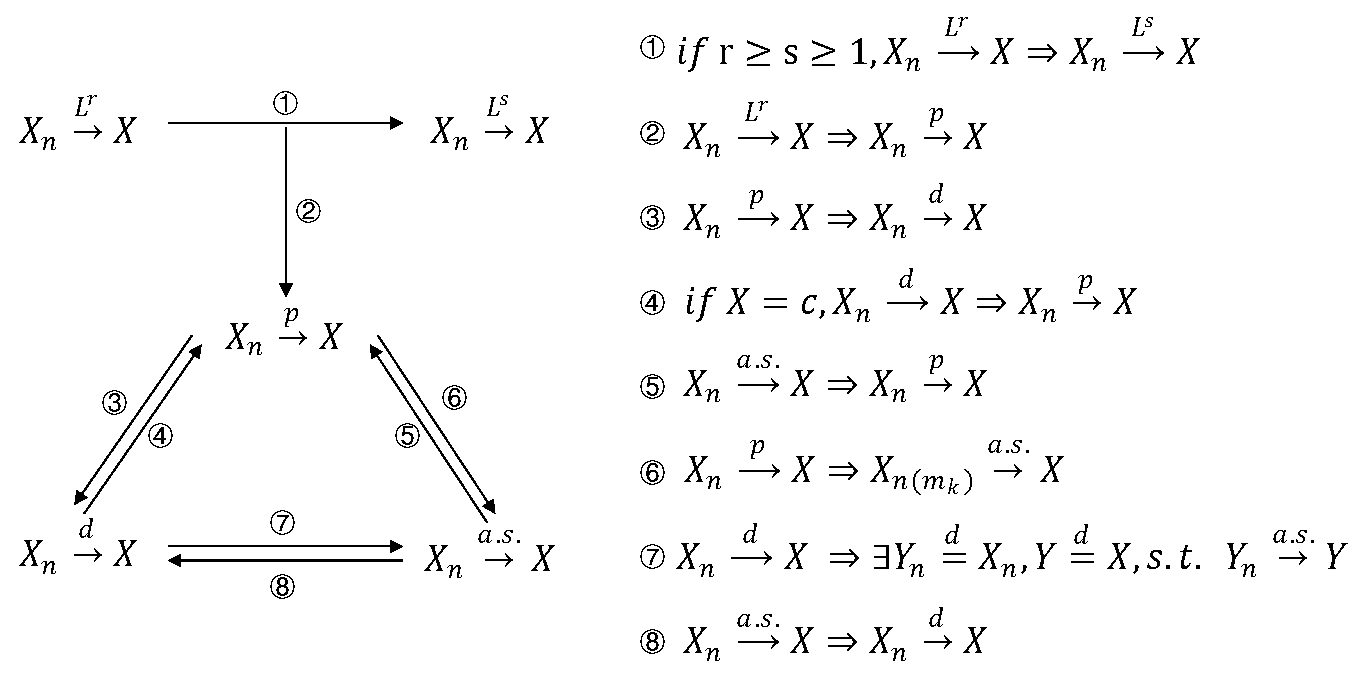
\includegraphics[width=0.9\textwidth]{./probability-theory/figures/relation-of-convergences.eps}
    \caption{Relations of Convergence of Random Variables}
\end{figure}

\section{Asymptotic Notation for Random Variables}

\begin{definition}
    A sequence $\{A_n\}$ of real-valued random variables is of smaller order in probability than a sequence $\{B_n\}$, if
    \begin{equation}
        \frac{A_n}{B_n}\stackrel{p}{\rightarrow}0.
    \end{equation}
    Smaller order in probability is denoted by
    \begin{equation}
        A_n=o_p(B_n).
    \end{equation}
    Particularly,
    \begin{equation}
        A_n=o_p(1)\iff A_n\stackrel{p}{\rightarrow}0.
    \end{equation}
\end{definition}

\begin{definition}
    A sequence $\{A_n\}$ of real-valued random variables is of smaller order than or equal to a sequence $\{B_n\}$ in probability, if
    \begin{equation}
        \forall\varepsilon>0\;\exists M_\varepsilon,\quad\lim_{n\rightarrow\infty} P\left(|A_n|\leq M_\varepsilon|B_n|\right)\geq 1-\varepsilon.
    \end{equation}
    Smaller order than or equal to in probability is denoted by
    \begin{equation}
        A_n=O_p(B_n).
    \end{equation}
\end{definition}

\begin{definition}
    A sequence $\{A_n\}$ of real-valued random variables is of the same order as a sequence $\{B_n\}$ in probability, if
    \begin{equation}
        \forall\varepsilon>0\;\exists m_{\varepsilon}<M_{\varepsilon},\quad\lim_{n\rightarrow\infty} P\left(m_{\varepsilon}<\frac{|A_{n}|}{|B_{n}|}<M_{\varepsilon}\right)\geq 1-\varepsilon.
    \end{equation}
    Same order in probability is denoted by
    \begin{equation}
        A_{n}\asymp_{p}B_{n}.
    \end{equation}
\end{definition}
\chapter{Law of Large Numbers}

\begin{introduction}
    \item Weak Law of Large Numbers
    \item Strong Law of Large Numbers
    \item Uniform Law of Large Numbers
\end{introduction}

\section{Weak Law of Large Numbers}

\begin{lemma}{}{}
    If $p>0$ and $E\left|Z_{n}\right|^{p}\rightarrow 0$, then
    \begin{equation}
        Z_{n}\stackrel{d}{\rightarrow}0.
    \end{equation}
\end{lemma}

\begin{proof}
    
\end{proof}

\begin{theorem}{Weak Law of Large Numbers with Finite Variances}{}
    Let $X_1,X_2,\ldots$ be i.i.d. random variables with $EX_i=\mu$ and $\text{Var}(X_i)\leq C<\infty$. Suppose $S_n=X_1+X_2+\ldots+X_n$, then
    \begin{equation}
        S_n/n\stackrel{L^2}{\rightarrow}\mu,\quad S_n/n\stackrel{p}{\rightarrow}\mu.
    \end{equation}
\end{theorem}

\begin{proof}
    
\end{proof}

\begin{theorem}{Weak Law of Large Numbers without i.i.d.}{}
    Let $X_1,X_2,\ldots$ be random variables, Suppose $S_n=X_1+X_2+\ldots+X_n$, $\mu_n=ES_n$, $\sigma_n^2=\text{Var}(S_n)$, if $\sigma_n^2/b_n^2\rightarrow 0$, then
    \begin{equation}
        \frac{S_n-\mu_n}{b_n}\stackrel{p}{\rightarrow}0.
    \end{equation}
\end{theorem}

\begin{proof}
    
\end{proof}

\begin{theorem}{Weak Law of Large Numbers for Triangular Arrays}{}
    For each $n$, let $X_{n,m},1\leq m\leq n$, be independent random variables. Suppose $b_n>0$ with $b_n\rightarrow\infty$, $\bar{X}_{n,m}=X_{n,m}I_{\left(X_{n,m}\leq b_n\right)}$, if
    \begin{enumerate}
        \item $\sum_{m=1}^{n}P\left(\left|X_{n,m}\right|>b_{n}\right)\rightarrow 0$, and
        \item $b_{n}^{-2}\sum_{m=1}^{n}E\bar{X}_{n,m}^{2}\rightarrow 0$.
    \end{enumerate}
    Suppose $S_{n}=X_{n, 1}+\cdots+X_{n,n}$ and $a_{n}=\sum_{m=1}^{n}E\bar{X}_{n,m}$, thenxxs
    \begin{equation}
        \frac{S_n-a_n}{b_n}\stackrel{p}{\rightarrow}0.
    \end{equation}
\end{theorem}

\begin{proof}
    
\end{proof}

\begin{theorem}{Weak Law of Large Numbers by Feller}{}
    Let $X_1,X_2,\ldots$ be i.i.d. random variables with
    \begin{equation}
        \lim_{x\rightarrow 0}xP(|X_i|>x)=0.
    \end{equation}
    Suppose $S_n=X_1+X_2+\ldots+X_n$, $\mu_n=E\left(X_1I_{(|X_1|<n)}\right)$, then
    \begin{equation}
        S_n/n-\mu_n\stackrel{p}{\rightarrow}0.
    \end{equation}
\end{theorem}

\begin{proof}
    
\end{proof}

\begin{theorem}{Weak Law of Large Numbers}{WLLN}
    Let $X_1,X_2,\ldots$ be i.i.d. random variables with $E|X_i|<\infty$. Suppose $S_n=X_1+X_2+\ldots+X_n$, $\mu=EX_i$, then
    \begin{equation}
        S_n/n\stackrel{p}{\rightarrow}\mu.
    \end{equation}
\end{theorem}

\begin{proof}
    
\end{proof}

\begin{note}
    $E|X_i|=\infty$
\end{note}

\section{Strong Law of Large Numbers}

\subsection{Borel-Cantelli Lemmas}

\begin{lemma}{Borel-Cantelli Lemma}{borel-cantelli-lemma}
    If $\sum_{n=1}^{\infty}P\left(A_{n}\right)<\infty$, then
    \begin{equation}
        P\left(A_{n}\text{ i.o. }\right)=0.
    \end{equation}
\end{lemma}

\begin{lemma}{The Second Borel-Cantelli Lemma}{}
    If $\{A_n\}$ are independent with $\sum_{n=1}^{\infty}P\left(A_{n}\right)=\infty$, then,
    \begin{equation}
        P\left(A_{n}\text{ i.o. }\right)=1.
    \end{equation}
\end{lemma}

\begin{corollary}{}{}
    Suppose $\{A_{n}\}$ are independent with $P\left(A_{n}\right)<1,\forall n$. If $P\left(\cup_{n=1}^{\infty}A_{n}\right)=1$ then
    \begin{equation}
        \sum_{n=1}^{\infty}P\left(A_{n}\right)=\infty,
    \end{equation}
    and hence $P\left(A_{n}\text{ i.o. }\right)=1$
\end{corollary}

\begin{proof}

\end{proof}

\subsection{Strong Law of Large Numbers}

\begin{theorem}{Strong Law of Large Numbers}{SLLN}
    Let $X_1,X_2,\ldots$ be i.i.d. random variables with $E|X_i|<\infty$. Suppose $S_n=X_1+X_2+\ldots+X_n$, $\mu=EX_i$, then
    \begin{equation}
        S_n/n\stackrel{a.s.}{\rightarrow}\mu.
    \end{equation}
\end{theorem}

\section{Uniform Law of Large Numbers}

\begin{theorem}{Uniform Law of Large Numbers}{ULLN}
    Suppose
    \begin{enumerate}
        \item $\Theta$ is compact.
        \item $g\left(X_{i},\theta\right)$ is continuous at each $\theta\in\Theta$ almost sure.
        \item $g\left(X_{i},\theta\right)$ is dominated by a function $G\left(X_{i}\right)$, i.e. $\left|g\left(X_{i},\theta\right)\right|\leq G\left(X_{i}\right)$.
        \item $EG\left(X_{i}\right)<\infty$.
    \end{enumerate}
    Then
    \begin{equation}
        \sup_{\theta\in\Theta}\left|n^{-1}\sum_{i=1}^{n}g\left(X_{i},\theta\right)-Eg\left(X_{i},\theta\right)\right|\stackrel{p}{\rightarrow}0.
    \end{equation}
\end{theorem}

\begin{proof}
    
\end{proof}

\chapter{Central Limit Theorems}

% \begin{introduction}
%     \item Classic Central Limit Theorem
%     \item Central Limit Theorem for independent non-identical Random Variables
%     \item Central Limit Theorem for dependent Random Variables
% \end{introduction}

\section{Classic Central Limit Theorem}

\subsection{The De Moivre-Laplace Theorem}

\begin{lemma}[Stirling's Formula] \label{lem:stirling}
    \begin{equation}
        n ! \sim \sqrt{2 \pi} n^{n+\frac{1}{2}} e^{-n} \text{ as } n \rightarrow \infty.
    \end{equation}
\end{lemma}

\begin{proof}

\end{proof}

\begin{lemma} \label{lem:exp}
    If $c_j\rightarrow 0$, $a_j\rightarrow\infty$ and $a_jc_j\rightarrow\lambda$, then
    \begin{equation}
        \left(1+c_j\right)^{a_j}\rightarrow e^\lambda.
    \end{equation}
\end{lemma}

\begin{proof}

\end{proof}

\begin{theorem}[The De Moivre-Laplace Theorem] \label{thm:de-moivre-laplace}
    Let $X_{1}, X_{2}, \ldots$ be i.i.d. with $P\left(X_{1}=1\right)=P\left(X_{1}=-1\right)=1 / 2$ and let $S_{n}=X_{1}+\cdots+X_{n}$. If $a<b$, then as $m \rightarrow \infty$
    \begin{equation}
        P\left(a \leq S_{m} / \sqrt{m} \leq b\right) \rightarrow \int_{a}^{b}(2 \pi)^{-1 / 2} e^{-x^{2} / 2} \mathrm{d} x.
    \end{equation}
\end{theorem}

\begin{proof}
    If $n$ and $k$ and integers
    \begin{equation*}
        P\left(S_{2 n}=2 k\right)=\left(\begin{array}{c}
                2 n \\
                n+k
            \end{array}\right) 2^{-2 n}
    \end{equation*}
    By lemma \ref{lem:stirling}, we have
    \begin{equation*}
        \begin{aligned}
            \left(\begin{array}{c}
                    2 n \\
                    n+k
                \end{array}\right) & =\frac{(2 n) !}{(n+k) !(n-k) !}                                                                                             \\
                                                   & \sim \frac{(2 n)^{2 n}}{(n+k)^{n+k}(n-k)^{n-k}} \cdot \frac{(2 \pi(2 n))^{1 / 2}}{(2 \pi(n+k))^{1 / 2}(2 \pi(n-k))^{1 / 2}}
        \end{aligned}
    \end{equation*}
    Hence,
    \begin{equation*}
        \begin{aligned}
            P\left(S_{2 n}=2 k\right) & =
            \left(\begin{array}{c}
                    2 n \\
                    n+k
                \end{array}\right) 2^{-2 n}                                                                                               \\
                                      & \sim\left(1+\frac{k}{n}\right)^{-n-k} \cdot\left(1-\frac{k}{n}\right)^{-n+k}                                      \\
                                      & \cdot(\pi n)^{-1 / 2} \cdot\left(1+\frac{k}{n}\right)^{-1 / 2} \cdot\left(1-\frac{k}{n}\right)^{-1 / 2}           \\
                                      & =\left(1-\frac{k^{2}}{n^{2}}\right)^{-n} \cdot\left(1+\frac{k}{n}\right)^{-k} \cdot\left(1-\frac{k}{n}\right)^{k} \\
                                      & \cdot(\pi n)^{-1 / 2} \cdot\left(1+\frac{k}{n}\right)^{-1 / 2} \cdot\left(1-\frac{k}{n}\right)^{-1 / 2}           \\
        \end{aligned}
    \end{equation*}
    Let $2k=x\sqrt{2n}$, i.e., $k=x\sqrt{\frac{n}{2}}$. By lemma \ref{lem:exp}, we have
    \begin{equation*}
        \begin{aligned}
            \left(1-\frac{k^{2}}{n^{2}}\right)^{-n} & =\left(1-x^{2} / 2 n\right)^{-n} \rightarrow e^{x^{2} / 2}       \\
            \left(1+\frac{k}{n}\right)^{-k}         & =(1+x / \sqrt{2 n})^{-x \sqrt{n / 2}} \rightarrow e^{-x^{2} / 2} \\
            \left(1-\frac{k}{n}\right)^{k}          & =(1-x / \sqrt{2 n})^{x \sqrt{n / 2}} \rightarrow e^{-x^{2} / 2}
        \end{aligned}
    \end{equation*}
    For this choice of $k$, $k/n \rightarrow 0$, so
    \begin{equation*}
        \left(1+\frac{k}{n}\right)^{-1 / 2} \cdot\left(1-\frac{k}{n}\right)^{-1 / 2} \rightarrow 1.
    \end{equation*}
    Putting things together, we have
    \begin{equation*}
        P\left(S_{2 n}=2 k\right) \sim (\pi n)^{-1 / 2} e^{-x^{2} / 2}, \text{ as } \frac{2k}{\sqrt{2n}} \rightarrow x.
    \end{equation*}
    Therefore,
    \begin{equation*}
        P\left( a\sqrt{2n} \leq S_{2 n} \leq b\sqrt{2 n} \right) = \sum_{m \in \left[a\sqrt{2 n},b\sqrt{2 n}\right] \cap 2\mathbb{Z}} P\left(S_{2 n}=m\right)
    \end{equation*}
    Let $m=x\sqrt{2 n}$, we have that this is
    \begin{equation*}
        \approx \sum_{x \in \left[a,b\right] \cap \left(2\mathbb{Z} / \sqrt{2 n}\right)}(2 \pi)^{-1 / 2} e^{-x^{2} / 2}\cdot(2/n)^{1/2}
    \end{equation*}
    where $2\mathbb{Z} / \sqrt{2 n} = \left\{2z/\sqrt{2n} : z\in\mathbb{Z}\right\}$. As $n\rightarrow\infty$, the sum just shown is
    \begin{equation*}
        \approx \int_{a}^{b}(2 \pi)^{-1 / 2} e^{-x^{2} / 2} \mathrm{d} x.
    \end{equation*}
    To remove the restriction to even integers, observe $S_{2 n +1}=S_{2 n} \pm 1$.\\
    Let $m=2n$, as $m\rightarrow\infty$,
    \begin{equation*}
        P\left(a \leq S_{m} / \sqrt{m} \leq b\right) \rightarrow \int_{a}^{b}(2 \pi)^{-1 / 2} e^{-x^{2} / 2} \mathrm{d} x.
    \end{equation*}
\end{proof}

\subsection{Classic Central Limit Theorem}

\begin{theorem}[Classic Central Limit Theorem (i.i.d.)]
    Let $X_1,X_2,\ldots$ be i.i.d. with $EX_i=\mu$, $\text{Var}(X_i)=\sigma^2<\infty$. Let $S_n=X_1+X_2+\ldots+X_n$, then
    \begin{equation}
        \frac{S_n-n\mu}{\sigma n^{\frac{1}{2}}} \stackrel{d}{\rightarrow} \chi,
    \end{equation}
    where $\chi$ has the standard normal distribution.
\end{theorem}

\begin{proof}

\end{proof}

\begin{theorem}[The Linderberg-Feller Central Limit Theorem]
    For each $n$, let $X_{n,m},1\leq m\leq n$, be independent random variables with $EX_{n,m}=0$. If
    \begin{enumerate}
        \item $\sum_{m=1}^{n}EX_{n,m}^{2} \rightarrow \sigma^{2}>0$.
        \item $\forall\epsilon>0,\lim_{n\rightarrow\infty}\sum_{m=1}^{n}E\left(\left|X_{n,m}\right|^{2};\left|X_{n,m}\right|>\epsilon\right)=0$
    \end{enumerate}
    Then $S_{n}=X_{n,1}+\cdots+X_{n,n}\stackrel{d}{\rightarrow}\sigma\chi$ as $n\rightarrow\infty$.
\end{theorem}

\subsection{Berry-Esseen Theorem}

\begin{theorem}[Berry-Esseen Theorem]
    Let $X_{1},X_{2},\ldots,X_{n}$ be i.i.d. with distribution $F$ , which has a mean $\mu$ and a finite third moment $\sigma^{3}$, then there exists a constant $C$ (independent of $F$),
    \begin{equation}
        \left|G_{n}(x)-\Phi(x)\right|\leq\frac{C}{\sqrt{n}}\frac{E\left|X_{1}-\mu\right|^{3}}{\sigma^{3}},\quad\forall x.
    \end{equation}
\end{theorem}

\begin{corollary}
    Under the assumptions of Theorem 51 ,
    $$
        G_{n}(x) \rightarrow \Phi(x) \text { as } n \rightarrow \infty
    $$
    for any sequence $F_{n}$ with mean $\xi_{n}$ and variance $\sigma_{n}^{2}$ for which
    $$
        \frac{E_{n}\left|X_{1}-\xi_{n}\right|^{3}}{\sigma_{n}^{3}}=o(\sqrt{n})
    $$
    and thus in particular if $(72)$ is bounded. Here $E_{n}$ denotes the expectation under $F_{n}$.
\end{corollary}

\section{Central Limit Theorem for independent non-identical Random Variables}

\begin{theorem}[The Liapounov Central Limit Theorem]

\end{theorem}

\section{Central Limit Theorem for Dependent Random Variables}


\chapter{The Delta Methods}

\begin{theorem}[Delta Method]
    Let $\{X_{n}\}$ be a sequence of random variables with
    \begin{equation*}
        \sqrt{n}\left[X_{n}-\theta\right] \stackrel{d}{\rightarrow}\sigma\chi,
    \end{equation*}
    where $\theta$ and $\sigma$ are finite, then for any function $g$ with the property that $g'(\theta)$ exists and is non-zero valued,
    \begin{equation*}
        \sqrt{n}\left[g\left(X_{n}\right)-g(\theta)\right] \stackrel{d}{\rightarrow} \sigma g'(\theta)\chi.
    \end{equation*}
\end{theorem}

\begin{proof}
    Under the assumption that $g'(\theta)$ is continuous.

    Since, $g'(\theta)$ exists, with the first-order Taylor Approximation:
    \begin{equation*}
        g(X_n)=g(\theta)+g'(\tilde{\theta})(X_n-\theta),
    \end{equation*}
    where $\tilde{\theta}$ lies between $X_n$ and $\theta$.

    Since $X_n\stackrel{p}{\rightarrow}\theta$, and $|\tilde{\theta}-\theta|<|X_n-\theta|$, then
    \begin{equation*}
        \tilde{\theta}\stackrel{p}{\rightarrow}\theta,
    \end{equation*}
    Since $g'(\theta)$ is continuous, by Continuous Mapping Theorem (\ref{thm:continuous-mapping-theorem}),
    \begin{equation*}
        g'(\tilde{\theta})\stackrel{p}{\rightarrow}g'(\theta).
    \end{equation*}
    and,
    \begin{equation*}
        \sqrt{n}\left(g(X_n)-g(\theta)\right)=\sqrt{n}g'(\tilde{\theta})(X_n-\theta),
    \end{equation*}
    \begin{equation*}
        \sqrt{n}\left[X_{n}-\theta\right] \stackrel{d}{\rightarrow}\sigma\chi,
    \end{equation*}
    by Slutsky's Theorem (\ref{thm:slutsky-theorem}),
    \begin{equation*}
        \sqrt{n}\left[g\left(X_{n}\right)-g(\theta)\right] \stackrel{d}{\rightarrow} \sigma g'(\theta)\chi.
    \end{equation*}
\end{proof}

\chapter{Exercises for Probability Theory and Examples}

\section{Measure Theory}

\begin{exercise}
    \begin{enumerate}
        \item Show that if $\mathcal{F}_{1}\subset \mathcal{F}_{2}\subset\ldots$ are $\sigma$ -algebras, then $\cup_{i}\mathcal{F}_{i}$ is an algebra.
        \item Give an example to show that $\cup_{i}\mathcal{F}_{i}$ need not be a $\sigma$ -algebra.
    \end{enumerate}
\end{exercise}

\begin{proof}
    \begin{enumerate}
        \item
              \textbf{Complement}: Suppose $A\in\cup_{i}\mathcal{F}_{i}$, since $\mathcal{F}_{1}\subset \mathcal{F}_{2}\subset\ldots$, assume $A\in\mathcal{F}_{i}$. And each $\mathcal{F}_{i}$ is $\sigma$-algebra,
              \begin{equation*}
                  A^c\in\mathcal{F}_{i}\subset\cup_{i}\mathcal{F}_{i}.
              \end{equation*}
              \textbf{Finite Union}: Suppose $A_1,A_2\in\cup_{i}\mathcal{F}_{i}$, since $\mathcal{F}_{1}\subset \mathcal{F}_{2}\subset\ldots$, assume $A_1\in\mathcal{F}_{i},A_2\in\mathcal{F}_{j}$, such that,
              \begin{equation*}
                  A_1,A_2\in\mathcal{F}_{\max(i,j)}.
              \end{equation*}
              Since each $\mathcal{F}_{i}$ is $\sigma$-algebra,
              \begin{equation*}
                  A_1\cup A_2\in\mathcal{F}_{i}\subset\cup_{i}\mathcal{F}_{i}.
              \end{equation*}
        \item
              Let $\mathcal{F}_{i}$ be a Borel Set of $[1,2-\frac{1}{i}]$. Suppose $A_i=[1,2-\frac{1}{i}]\in\mathcal{F}_{i}$,
              \begin{equation*}
                  \cup_{i}A_{i}=[1,2)\notin\cup_{i}\mathcal{F}_{i}.
              \end{equation*}
    \end{enumerate}
\end{proof}

\section{Laws of Large Numbers}

\section{Central Limit Theorems}

\begin{exercise}
    Let $g\geq 0$ be continuous. If $X_{n}\stackrel{d}{\rightarrow}X_{\infty},$ then
    \begin{equation*}
        \liminf_{n\rightarrow\infty}Eg\left(X_{n}\right)\geq Eg\left(X_{\infty}\right).
    \end{equation*}
    \label{ex:fatou-lemma-distribution}
\end{exercise}

\begin{proof}
    Let $Y_n\stackrel{d}{=}X_n,1\leq n\leq\infty$ with $Y_n\stackrel{a.s.}{\rightarrow}Y_\infty$ (Lemma \ref{lem:distribution-to-probability}).
    Since $g\geq 0$ be continuous, $g(Y_n)\stackrel{a.s.}{\rightarrow}g(Y_\infty)$ and $g(Y_n)\geq 0$ (Theorem \ref{thm:continuous-mapping-theorem}), and the Fatou's Lemma (\ref{thm:fatou-lemma}) implies,
    \begin{equation*}
        \begin{aligned}
            \liminf_{n\rightarrow\infty}Eg(X_n)= & \liminf_{n\rightarrow\infty}Eg(Y_n)\geq E\left(\liminf_{n\rightarrow\infty}g(Y_n)\right) \\
            =                                    & Eg(Y_\infty)=Eg(X_\infty).
        \end{aligned}
    \end{equation*}
\end{proof}

\begin{exercise}
    Suppose $g,h$ are continuous with $g(x)>0$, and $|h(x)|/g(x)\rightarrow 0$ as $|x|\rightarrow\infty$. If $F_{n}\stackrel{d}{\rightarrow}F$ and $\int g(x)\mathrm{d}F_{n}(x)\leq C<\infty,$ then
    \begin{equation*}
        \int h(x)\mathrm{d}F_{n}(x) \rightarrow \int h(x)\mathrm{d}F(x).
    \end{equation*}
\end{exercise}

\begin{proof}
    \begin{equation*}
        \begin{aligned}
            \left|\int h(x)\mathrm{d}F_{n}(x)-\int h(x)\mathrm{d}F(x)\right| = & \left|{\int_{x\in[-M,M]}h(x)\mathrm{d}F_{n}(x)+\int_{x\notin[-M,M]}h(x)\mathrm{d}F_{n}(x)}\right. \\
                                                                               & \left.{-\int_{x\in[-M,M]}h(x)\mathrm{d}F(x)-\int_{x\notin[-M,M]}h(x)\mathrm{d}F(x)}\right|        \\
            \leq                                                               & \left|\int_{x\in[-M,M]}h(x)\mathrm{d}F_{n}(x)-\int_{x\in[-M,M]}h(x)\mathrm{d}F(x)\right|          \\
                                                                               & + \left|\int_{x\notin[-M,M]}h(x)\mathrm{d}F_{n}(x)-\int_{x\notin[-M,M]}h(x)\mathrm{d}F(x)\right|
        \end{aligned}.
    \end{equation*}

    Let $X_n,1\leq n<\infty$, with distribution $F_n$, so that $X_n\stackrel{a.s.}{\rightarrow}X$ (Lemma \ref{lem:distribution-to-probability}).
    \begin{equation*}
        \left|\int_{x\in[-M,M]}h(x)\mathrm{d}F_{n}(x)-\int_{x\in[-M,M]}h(x)\mathrm{d}F(x)\right| = \left|E\left(h(X_n)-h(X)\right)I_{x\in[-M,M]}\right|.
    \end{equation*}

    By Continuity Mapping Theorem (\ref{thm:continuous-mapping-theorem}), $\lim_{n\rightarrow\infty}\left|E\left(h(X_n)-h(X)\right)I_{x\in[-M,M]}\right| = 0$.

    Since
    \begin{equation*}
        h(x)I_{x\notin[-M,M]}\leq g(x)\sup_{x\notin[-M,M]}\frac{h(x)}{g(x)},
    \end{equation*}
    and by Exercise \ref{ex:fatou-lemma-distribution}
    \begin{equation*}
        Eg(X) \leq \liminf_{n\rightarrow\infty}Eg(X_n)=\liminf_{n\rightarrow\infty}\int g(x)\mathrm{d}F_{n}(x)\leq C<\infty,
    \end{equation*}
    \begin{equation*}
        \begin{aligned}
            \left|\int_{x\notin[-M,M]}h(x)\mathrm{d}F_{n}(x)-\int_{x\notin[-M,M]}h(x)\mathrm{d}F(x)\right| = \left|E\left(h(X_n)-h(X)\right)I_{x\notin[-M,M]}\right| \\
            \leq 2E\max(h(Xn),h(X))I_{x\notin[-M,M]}\leq 2C\sup_{x\notin[-M,M]}\frac{h(x)}{g(x)}.                                                                    \\
        \end{aligned}
    \end{equation*}

    Hence, let $M\rightarrow\infty$,
    \begin{equation*}
        \lim_{n\rightarrow\infty}\left|\int h(x)\mathrm{d}F_{n}(x)-\int h(x)\mathrm{d}F(x)\right| \leq 2C\sup_{x\notin[-M,M]}\frac{h(x)}{g(x)}\rightarrow 0,
    \end{equation*}
    which means,
    \begin{equation*}
        \int h(x)\mathrm{d}F_{n}(x) \rightarrow \int h(x)\mathrm{d}F(x).
    \end{equation*}
\end{proof}

\begin{exercise}
    Let $X_{1},X_{2},\ldots$ be i.i.d. with $EX_{i}=0$ and $EX_{i}^{2}=\sigma^{2}\in(0,\infty)$. Then
    \begin{equation*}
        \sum_{m=1}^{n}X_{m}/\left(\sum_{m=1}^{n}X_{m}^{2}\right)^{1/2}\stackrel{d}{\rightarrow}\chi.
    \end{equation*}
\end{exercise}

\begin{exercise}
    Show that if $\left|X_{i}\right|\leq M$ and $\sum_{n}\text{Var}\left(X_{n}\right)=\infty$, then
    \begin{equation*}
        \left(S_{n}-E S_{n}\right)/\sqrt{\text{Var}\left(S_{n}\right)}\stackrel{d}{\rightarrow}\chi.
    \end{equation*}
\end{exercise}

\begin{exercise}
    Suppose $EX_{i}=0,EX_{i}^{2}=1$ and $E\left|X_{i}\right|^{2+\delta}\leq C$ for some $0<\delta,C<\infty$. Show that
    \begin{equation*}
        S_{n}/\sqrt{n}\stackrel{d}{\rightarrow}\chi.
    \end{equation*}
\end{exercise}
\part{Stochastic Process}
\chapter{Martingales}

\section{Conditional Expectation}

\begin{definition}[Conditional Expectation]

\end{definition}

\begin{example}
    \begin{enumerate}
        \item
    \end{enumerate}
\end{example}

\begin{property}
    
\end{property}

\section{Martingales}

Let $\mathcal{F}_{n}$ be a filtration, i.e., an increasing sequence of $\sigma$-fields.
\begin{definition}[Martingale]
    A sequence $\left\{X_{n}\right\}$ of real-valued random variables  is said to be a martingale with respect to $\mathcal{F}_{n}$, if
    \begin{enumerate}
        \item $X_{n}$ is integrable, i.e., $E\left|X_{n}\right|<\infty$
        \item $X_{n}$ is adapted to $\mathcal{F}_{n}$, i.e., $\forall n,X_{n}\in \mathcal{F}_{n}$
        \item $X_{n}$ satisfies the martingale condition, i.e.,
              \begin{equation}
                  E\left(X_{n+1}\mid\mathcal{F}_{n}\right)=X_{n},\quad\forall n
              \end{equation}
    \end{enumerate}
\end{definition}

\begin{note}
    If in the last definition $=$ is replaced by $\leq$ or $\geq$, then $X$ is said to be a supermartingale or submartingale, respectively.
\end{note}

\begin{example}[ Linear Martingale]
    
\end{example}

\begin{example}[ Quadratic Martingale]
    
\end{example}

\begin{example}[ Random Walk]
    Suppose $X_{n}=X_{0}+\xi_{1}+\cdots+\xi_{n}$, where $X_{0}$ is constant, $\xi_{m}$ are independent and have $E\xi_{m}=0,\sigma_{m}^{2}=E\xi_{m}^{2}<\infty$. Let $\mathcal{F}_{n}=\sigma\left(\xi_{1},\ldots,\xi_{n}\right)$ for $n\geq 1$ and take $\mathcal{F}_{0}=\{\emptyset, \Omega\}$. Show $X_{n}$ is a martingale, and $X_{n}^{2}$ is a submartingale.
\end{example}

\begin{proof}
    It is obvious that,
    \begin{equation*}
        E\left|X_{n}\right|<\infty,\quad X_{n}\in\mathcal{F}_{n}
    \end{equation*}
    Since $\xi_{n+1}$ is independent of $\mathcal{F}_{n}$, so using the linearity of conditional expectation, (4.1.1), and Example 4.1.4,
    \begin{equation*}
        E\left(X_{n+1}\mid\mathcal{F}_{n}\right)=E\left(X_{n}\mid\mathcal{F}_{n}\right)+E\left(\xi_{n+1}\mid\mathcal{F}_{n}\right)=X_{n}+E\xi_{n+1}=X_{n}
    \end{equation*}
    So $X_{n}$ is a martingale, and Theorem 4.2.6 implies $X_{n}^{2}$ is a submartingale.
\end{proof}

\begin{note}
    If we let $\lambda=x^{2}$ and apply Theorem 4.4.2 to $X_{n}^{2}$, we get Kolmogorov's maximal inequality, Theorem 2.5.5:
    \begin{equation}
        P\left(\max_{1\leq m\leq n}\left|X_{m}\right|\geq x\right)\leq x^{-2}\operatorname{var}\left(X_{n}\right)
    \end{equation}
\end{note}

\section{Doob's Inequality}

\begin{theorem}[Doob's Decomposition]

\end{theorem}

\begin{theorem}[Doob's Inequality]

\end{theorem}

\begin{theorem}[$L^{p}$ Maximum Inequality]

\end{theorem}

\section{Uniform Integrability}

\section{Optional Stopping Theorems}

\chapter{Markov Chains}

\section{Markov Chain}

\begin{definition}[Markov Chain, Simple]
    A sequence $\left\{X_{n}\right\}$ of real-valued random variables  is said to be a Markov chain, if for any states $i_{0},\ldots i_{n-1},i$, and $j$
    \begin{equation}
        P\left(X_{n+1}=j\mid X_{n}=i,X_{n-1}=i_{n-1},\ldots X_{0}=i_{0}\right)=P\left(X_{n+1}=j\mid X_{n}=i\right)
    \end{equation}
    and the transition probability is
    \begin{equation}
        p(i,j)=P\left(X_{n+1}=j\mid X_{n}=i\right)
    \end{equation}
\end{definition}

\begin{example}[ Random Walk]
    Suppose $X_{n}=X_{0}+\xi_{1}+\cdots+\xi_{n}$, where $X_{0}$ is constant, $\xi_{m}\in\mathbb{Z}^{d}$ are independent with distribution $\mu$. Show $X_{n}$ is a Markov chain with transition probability,
    \begin{equation*}
        p\left(i,j\right)=\mu\left(\left\{j-i\right\}\right)
    \end{equation*}
\end{example}

\begin{proof}
    Since $\xi_{m}$ are independent with distribution $\mu$,
    \begin{equation*}
        \begin{aligned}
              & P\left(X_{n+1}=j\mid X_{n}=i,X_{n-1}=i_{n-1},\ldots X_{0}=i_{0}\right)                                     \\
            = & P\left(X_{n}+\xi_{n+1}=j\mid X_{n}=i\right)=P\left(\xi_{n+1}=j-i\right)=\mu\left(\left\{j-i\right\}\right)
        \end{aligned}
    \end{equation*}
\end{proof}

\begin{definition}[Branching Processes]
    Let $\xi_{i}^{n},i,n\geq 1$, be i.i.d. nonnegative integer-valued random variables. Define a sequence $Z_{n},n\geq 0$ by $Z_{0}=1$ and
    \begin{equation}
        Z_{n+1}=\left\{\begin{array}{ll}
            \xi_{1}^{n+1}+\cdots+\xi_{Z_{n}}^{n+1} & Z_{n}>0 \\
            0                                      & Z_{n}=0
        \end{array}\right.
    \end{equation}
    $Z_{n}$ is called a Branching process.
\end{definition}

\begin{note}
    The idea behind the definitions is that $Z_{n}$ is the number of individuals in the $n$-th generation, and each member of the $n$-th generation gives birth independently to an identically distributed number of children.
\end{note}

\begin{example}[ Branching Processes]
    Show branching process is a Markov chain with transition probability,
    \begin{equation*}
        p(i,j)=P\left(\sum_{k=1}^{i}\xi_{k}=j\right)
    \end{equation*}
\end{example}

\begin{proof}
    Since $\xi_{k}^{n}$ are independent with identically distribution,
    \begin{equation*}
        \begin{aligned}
              & P\left(Z_{n+1}=j\mid Z_{n}=i,Z_{n-1}=i_{n-1},\ldots Z_{0}=i_{0}\right)                            \\
            = & P\left(\sum_{k=1}^{Z_{n}}\xi_{k}^{n+1}=j\mid Z_{n}=i\right)=P\left(\sum_{k=1}^{i}\xi_{k}=j\right)
        \end{aligned}
    \end{equation*}
\end{proof}

Suppose $(S, \mathcal{S})$ be a measurable space, which will be the state space for our Markov chain.

\begin{definition}[Transition Probability]
    A function $p:S\times\mathcal{S}\rightarrow\mathbf{R}$ is said to be a transition probability, if
    \begin{enumerate}
        \item For each $x\in S$, $A\rightarrow p(x,A)$ is a probability measure on $(S,\mathcal{S})$
        \item For each $A\in\mathcal{S}$, $x\rightarrow p(x,A)$ is a measurable function
    \end{enumerate}
\end{definition}
\begin{definition}[Markov Chain]
    A sequence $\left\{X_{n}\right\}$ of real-valued random variables with transition probability $p$ is said to be a Markov chain with respect to $\mathcal{F}_{n}$, if
    \begin{equation}
        P\left(X_{n+1}\in B\mid\mathcal{F}_{n}\right)=p\left(X_{n},B\right)
    \end{equation}
\end{definition}

\begin{remark}
    Given a transition probability $p$ and an initial distribution $\mu$ on $(S,\mathcal{S})$, the consistent set of finite dimensional distributions is
    \begin{equation}
        P\left(X_{j}\in B_{j},0\leq j\leq n\right)=\int_{B_{0}}\mu\left(\,\mathrm{d}x_{0}\right)\int_{B_{1}}p\left(x_{0},\,\mathrm{d}x_{1}\right)\cdots\int_{B_{n}}p\left(x_{n-1},\,\mathrm{d}x_{n}\right)
        F    \end{equation}
\end{remark}

\section{Markov Properties}

\begin{theorem}[Markov Property]

\end{theorem}

\begin{corollary}[Chapman-Kolmogorov Equation]

\end{corollary}

\begin{theorem}[Strong Markov Property]

\end{theorem}

\section{Recurrence and Transience}

Let $T_{y}^{0}=0$, and for $k\geq 1$, and
\begin{equation}
    T_{y}^{k}=\inf\left\{n>T_{y}^{k-1}:X_{n}=y\right\}
\end{equation}
then $T_{y}^{k}$ is the time of the $k$-th return to $y$, where $T_{y}^{1}>0$, so any visit at time 0 does not count.

Let
\begin{equation}
    \rho_{x y}=P_{x}\left(T_{y}<\infty\right)
\end{equation}
and we have
\begin{equation}
    P_{x}\left(T_{y}^{k}<\infty\right)=\rho_{xy}\rho_{yy}^{k-1}
\end{equation}

\begin{proof}

\end{proof}

Let
\begin{equation}
    N(y)=\sum_{n=1}^{\infty}1_{\left(X_{n}=y\right)}
\end{equation}
be the number of visits to $y$ at positive times.

\begin{definition}[Recurrent]
    A state $y$ is said to be recurrent if $\rho_{yy}=1$.
\end{definition}

\begin{property}
    The recurrent state $y$ has the following properties
    \begin{enumerate}
        \item $y$ is recurrent if and only if
              \begin{equation*}
                  E_{y}N(y)=\infty.
              \end{equation*}
        \item If $x$ is recurrent and $\rho_{xy}>0$, then $y$ is recurrent and $\rho_{yx}=1$.
    \end{enumerate}
\end{property}

\begin{definition}
    A state $y$ is said to be transient if $\rho_{yy}<1$.
\end{definition}

\begin{property}
    The transient state $y$ has the following properties
    \begin{enumerate}
        \item If $y$ is transient, then
              \begin{equation*}
                  E_{x}N(y)<\infty,\quad\forall x.
              \end{equation*}
    \end{enumerate}
\end{property}

\begin{proof}
    \begin{equation*}
        \begin{aligned}
            E_{x}N(y) & =\sum_{k=1}^{\infty}P_{x}(N(y)\geq k)=\sum_{k=1}^{\infty}P_{x}\left(T_{y}^{k}<\infty\right) \\
                      & =\sum_{k=1}^{\infty}\rho_{xy}\rho_{yy}^{k-1}=\frac{\rho_{xy}}{1-\rho_{yy}}<\infty
        \end{aligned}
    \end{equation*}
\end{proof}

\begin{definition}[Closed State Set]
    A set $C$ of states is said to be closed, if
    \begin{equation}
        x\in C,\rho_{xy}>0\Rightarrow y\in C.
    \end{equation}
\end{definition}

\begin{definition}[Irreducible State Set]
    A set $D$ of states is said to be irreducible, if
    \begin{equation}
        x,y\in D\Rightarrow\rho_{xy}>0.
    \end{equation}
\end{definition}

\begin{theorem}
    Let $C$ be a finite closed set, then
    \begin{enumerate}
        \item $C$ contains a recurrent state.
        \item If $C$ is irreducible, then all states in $C$ are recurrent.
    \end{enumerate}
\end{theorem}

\begin{theorem}
    Suppose $C_{x}=\left\{y:\rho_{x y}>0\right\}$, then $C_{x}$ is an irreducible closed set.
\end{theorem}

\begin{proof}
    If $y,z\in C_{x}$, then $\rho_{yz}\geq\rho_{yx}\rho_{xz}>0$. If $\rho_{yw}>0$, then $\rho_{xw}\geq\rho_{xy}\rho_{yw}>0$, so $w\in C_{x}$.
\end{proof}

\begin{example}[ A Seven-state Chain]
    Consider the transition probability,
    \begin{equation*}
        \begin{array}{cccccccc}
                       & \mathbf{1} & \mathbf{2} & \mathbf{3} & \mathbf{4} & \mathbf{5} & \mathbf{6} & \mathbf{7} \\
            \mathbf{1} & .3         & 0          & 0          & 0          & .7         & 0          & 0          \\
            \mathbf{2} & .1         & .2         & .3         & .4         & 0          & 0          & 0          \\
            \mathbf{3} & 0          & 0          & .5         & .5         & 0          & 0          & 0          \\
            \mathbf{4} & 0          & 0          & 0          & .5         & 0          & .5         & 0          \\
            \mathbf{5} & .6         & 0          & 0          & 0          & .4         & 0          & 0          \\
            \mathbf{6} & 0          & 0          & 0          & .1         & 0          & .1         & .8         \\
            \mathbf{7} & 0          & 0          & 0          & 1          & 0          & 0          & 0
        \end{array}
    \end{equation*}
    try to identify the states that are recurrent and those that are transient.
\end{example}

\begin{proof}
    $\{2,3\}$ are transition states, and $\{1,4,5,6,7\}$ are recurrent states.
\end{proof}

\begin{remark}
    Suppose $S$ is finite, for $x\in S$,
    \begin{enumerate}
        \item $x$ is transient, if
              \begin{equation*}
                  \exists y,\text{ s.t. }\quad\rho_{xy}>0,\rho_{yx}=0
              \end{equation*}
        \item $x$ is recurrent, if
              \begin{equation*}
                  \exists y,\text{ s.t. }\quad\rho_{xy}>0,\rho_{yx}>0
              \end{equation*}
    \end{enumerate}
\end{remark}

% Theorem 5.2.6 implies $P_{y}\left(T_{y}^{k}<\infty\right)=1$ for all $k$, so $P_{y}\left(X_{n}=y\text{ i.o. }\right)=1$.

\section{Stationary Measures}

\section{Asymptotic Behavior}

\section{Ergodic Theorems}

\begin{definition}[Stationary Sequence]

\end{definition}

\begin{theorem}[Ergodic Theorem]

\end{theorem}

\begin{example}

\end{example}
\chapter{Brownian Motion}

\begin{definition}[Brownian Motion (1)]
    A real-valued stochastic process $B(t),t\geq 0$ is said to be Brownian motion, if
    \begin{enumerate}
        \item for any $0=t_{0}\leq t_{1}\leq\ldots\leq t_{n}$ the increments
              \begin{equation*}
                  B\left(t_{1}\right)-B\left(t_{0}\right),\ldots,B\left(t_{n}\right)-B\left(t_{n-1}\right)
              \end{equation*}
              are independent
        \item for any $s,t\geq 0$ and Borel sets $A\in\mathbb{R}$,
              \begin{equation}
                  P\left(B(s+t)-B(s)\in A\right)=\int_{A}(2\pi t)^{-1/2}\exp\left(-x^{2}/2t\right)\,\mathrm{d}x
              \end{equation}
        \item the sample paths $t\rightarrow B(t)$ are a.s. continuous
    \end{enumerate}
\end{definition}

The one-dimensional Brownian motion has the following properties

\begin{property}
    Suppose $B(0)=0$, then we have
    \begin{enumerate}
        \item $EB_{t}=0,\operatorname{Var}\left(B_{t}\right)=t,\quad t\geq 0$.
        \item $\operatorname{Cov}\left(B_{s},B_{t}\right)=s,\operatorname{Corr}\left(B_{s},B_{t}\right)=\sqrt{\frac{s}{t}},\quad\forall 0\leq s\leq t$.
    \end{enumerate}
\end{property}

\begin{proof}
    \begin{enumerate}
        \item Since $B_{t}=B_{t}-B_{0}\sim N(0, t)$, then we have
              \begin{equation*}
                  EB_{t}=0,\operatorname{Var}\left(B_{t}\right)=t
              \end{equation*}
        \item Suppose $0\leq s\leq t$,
              \begin{equation*}
                  \operatorname{Cov}\left(B_{s}, B_{t}\right)=E\left[\left(B_{s}-EB_{s}\right)\left(B_{t}-EB_{t}\right)\right]=EB_{s}B_{t}
              \end{equation*}
              Let $B_{t}=\left(B_{t}-B_{s}\right)+B_{s}$, we have
              \begin{equation*}
                  \begin{aligned}
                      EB_{s}B_{t} & =E\left[B_{s}\cdot\left(\left(B_{t}-B_{s}\right)+B_{s}\right)\right] \\
                                  & =E\left[B_{s}\cdot\left(B_{t}-B_{s}\right)\right]+EB_{s}^{2}
                  \end{aligned}
              \end{equation*}
              Since $B_{s}=B_{s}-B_{0}$ and $B_{t}-B_{s}$ are independent,
              \begin{equation*}
                  E\left[B_{s} \cdot\left(B_{t}-B_{s}\right)\right]=EB_{s} \cdot E\left[B_{t}-B_{s}\right]=0
              \end{equation*}
              Thus
              \begin{equation*}
                  \operatorname{Cov}\left(B_{s}, B_{t}\right)=EB_{s}^{2}=s
              \end{equation*}
              And
              \begin{equation*}
                  \operatorname{Corr}\left(B_{s},B_{t}\right)=\frac{\operatorname{Cov}\left(B_{s},B_{t}\right)}{\sigma_{B_{s}}\sigma_{B_{t}}}=\frac{s}{\sqrt{st}}=\sqrt{\frac{s}{t}}
              \end{equation*}
    \end{enumerate}
\end{proof}

A second equivalent definition of Brownian motion are as followed,

\begin{definition}[Brownian Motion (2)]
    A real-valued stochastic process $B(t),t\geq 0$, \textbf{starting from $0$}, is said to be Brownian motion, if
    \begin{enumerate}
        \item $B(t)$ is a Gaussian process\footnote{Gaussian process, i.e., all its finite dimensional distributions are multivariate normal.}
        \item $\forall s,t\geq 0,EB_{s}=0$ and $EB_{s}B_{t}=s\wedge t$
        \item the sample paths $t\rightarrow B(t)$ are a.s. continuous
    \end{enumerate}
\end{definition}

\section{Markov Properties}

\section{Martingales}

\begin{example}
    Suppose $B_{t}$ is a Brownian motion, then $B_{t}^{2}-t$ is a martingale.
\end{example}

\begin{proof}
    Let $B_{t}^{2}=\left(B_{s}+B_{t}-B_{s}\right)^{2}$, we have
    \begin{equation*}
        \begin{aligned}
            E_{x}\left(B_{t}^{2}\mid\mathcal{F}_{s}\right) & =E_{x}\left(B_{s}^{2}+2 B_{s}\left(B_{t}-B_{s}\right)+\left(B_{t}-B_{s}\right)^{2} \mid \mathcal{F}_{s}\right)                            \\
                                                           & =B_{s}^{2}+2 B_{s} E_{x}\left(B_{t}-B_{s} \mid \mathcal{F}_{s}\right)+E_{x}\left(\left(B_{t}-B_{s}\right)^{2} \mid \mathcal{F}_{s}\right) \\
                                                           & =B_{s}^{2}+0+(t-s)
        \end{aligned}
    \end{equation*}
    since $B_{t}-B_{s}$ is independent of $\mathcal{F}_{s}$ and has mean 0 and variance $t-s$.
\end{proof}

\begin{example}
    Suppose $B_{t}$ is a Brownian motion, $\exp\left(\theta B_{t}-\left(\theta^{2}t/2\right)\right)$ is a martingale.
\end{example}

\begin{proof}
    Let $B_{t}=B_{t}-B_{s}+B_{s}$, then
    \begin{equation*}
        \begin{aligned}
            E_{x}\left(\exp\left(\theta B_{t}\right)\mid\mathcal{F}_{s}\right) & =\exp \left(\theta B_{s}\right)E\left(\exp\left(\theta\left(B_{t}-B_{s}\right)\right)\mid\mathcal{F}_{s}\right) \\
                                                                               & =\exp\left(\theta B_{s}\right)\exp\left(\theta^{2}(t-s)/2\right)
        \end{aligned}
    \end{equation*}
    since $B_{t}-B_{s}$ is independent of $\mathcal{F}_{s}$ and has mean 0 and variance $t-s$. Thus
    \begin{equation*}
        \begin{aligned}
            E_{x}\left(\exp\left(\theta B_{t}-\left(\theta^{2}t/2\right)\right)\mid\mathcal{F}_{s}\right) & =E_{x}\left(\exp\left(\theta B_{t}\right)\mid\mathcal{F}_{s}\right)\cdot\exp\left(-\left(\theta^{2}t/2\right)\right) \\
                                                                                                          & =\exp\left(\theta B_{s}-\left(\theta^{2}s/2\right)\right)
        \end{aligned}
    \end{equation*}
\end{proof}

\begin{theorem}[Lévy's Martingale Characterization]
    Let $B(t),t\geq 0$, be a real-valued stochastic process and let $\mathcal{F}_{t}=\sigma\left(B_{s},s\leq t\right)$ be the filtration generated by it. Then $B(t)$ is a Brownian motion if and only if
    \begin{enumerate}
        \item $B(0)=0$ a.s.
        \item the sample paths $t\rightarrow B(t)$ are continuous a.s.
        \item $B(t)$ is a martingale with respect to $\mathcal{F}_{t}$
        \item $|B(t)|^{2}-t$ is a martingale with respect to $\mathcal{F}_{t}$
    \end{enumerate}
\end{theorem}

\section{Sample Paths}

Let $0=t_{0}^{n}<t_{1}^{n}<\cdots<t_{n}^{n}=T$, where $t_{i}^{n}=\frac{iT}{n}$ be a partition of the interval $[0,T]$ into $n$ equal parts, and
\begin{equation}
    \Delta_{i}^{n}B=B\left(t_{i+1}^{n}\right)-B\left(t_{i}^{n}\right)
\end{equation}
be the corresponding increments of the Brownian motion $B(t)$.

\begin{theorem} \label{thm:limited-square-variation}
    \begin{equation}
        \lim_{n\rightarrow\infty}\sum_{i=0}^{n-1}\left(\Delta_{i}^{n}B\right)^{2}=T\quad\text { in }\quad L^{2}
    \end{equation}
\end{theorem}

\begin{proof}
    Since the increments $\Delta_{i}^{n}B$ are independent and
    \begin{equation*}
        E\left(\Delta_{i}^{n}B\right)=0,\quad E\left(\left(\Delta_{i}^{n}B\right)^{2}\right)=\frac{T}{n},\quad E\left(\left(\Delta_{i}^{n}B\right)^{4}\right)=\frac{3T^{2}}{n^{2}}
    \end{equation*}
    it follows that
    \begin{equation*}
        \begin{aligned}
            E\left(\left[\sum_{i=0}^{n-1}\left(\Delta_{i}^{n}B\right)^{2}-T\right]^{2}\right)= & E\left(\left[\sum_{i=0}^{n-1}\left(\left(\Delta_{i}^{n}B\right)^{2}-\frac{T}{n}\right)\right]^{2}\right)                                                   \\
            =                                                                                  & \sum_{i=0}^{n-1}E\left[\left(\left(\Delta_{i}^{n}B\right)^{2}-\frac{T}{n}\right)^{2}\right]                                                                \\
            =                                                                                  & \sum_{i=0}^{n-1}\left[E\left(\left(\Delta_{i}^{n}B\right)^{4}\right)-\frac{2T}{n}E\left(\left(\Delta_{i}^{n}B\right)^{2}\right)+\frac{T^{2}}{n^{2}}\right] \\
            =                                                                                  & \sum_{i=0}^{n-1}\left[\frac{3T^{2}}{n^{2}}-\frac{2T^{2}}{n^{2}}+\frac{T^{2}}{n^{2}}\right]                                                                 \\
            =                                                                                  & \frac{2T^{2}}{n}\rightarrow 0,\quad n\rightarrow\infty
        \end{aligned}
    \end{equation*}
\end{proof}

\begin{definition}[Variation]
    The variation of a function $f:[0,T]\rightarrow\mathbb{R}$ is defined to be
    \begin{equation}
        \limsup_{\Delta t\rightarrow 0}\sum_{i=0}^{n-1}\left|f\left(t_{i+1}\right)-f\left(t_{i}\right)\right|
    \end{equation}
    where $t=\left(t_{0},t_{1},\ldots,t_{n}\right)$ is a partition of $[0,T]$, i.e. $0=t_{0}<t_{1}<\cdots<t_{n}=T$, and where
    \begin{equation}
        \Delta t=\max_{i=0,\ldots,n-1}\left|t_{i+1}-t_{i}\right|
    \end{equation}
\end{definition}

\begin{theorem}
    The variation of the paths of $B(t)$ is infinite a.s..
\end{theorem}

\begin{proof}
    Consider the sequence of partitions $t^{n}=\left(t_{0}^{n},t_{1}^{n},\ldots,t_{n}^{n}\right)$ of $[0,T]$ into $n$ equal parts. Then
    \begin{equation*}
        \sum_{i=0}^{n-1}\left|\Delta_{i}^{n}B\right|^{2}\leq\left(\max_{i=0,\ldots,n-1}\left|\Delta_{i}^{n}B\right|\right)\sum_{i=0}^{n-1}\left|\Delta_{i}^{n}B\right|
    \end{equation*}

    Since the paths of $B(t)$ are a.s. continuous on $[0,T]$,
    \begin{equation*}
        \lim_{n\rightarrow\infty}\left(\max_{i=0,\ldots,n-1}\left|\Delta_{i}^{n}B\right|\right)=0\quad\text{ a.s. }
    \end{equation*}

    By Theorem \ref{thm:limited-square-variation}, we have
    \begin{equation*}
        \lim_{n\rightarrow\infty}\sum_{i=0}^{n-1}\left(\Delta_{i}^{n}B\right)^{2}=T\quad\text { in }\quad L^{2}
    \end{equation*}
    Since every sequence of random variables convergent in $L^{2}$ has a subsequence convergent a.s. There is a subsequence $t^{n_{k}}=\left(t_{0}^{n_{k}},t_{1}^{n_{k}},\ldots,t_{n_{k}}^{n_{k}}\right)$ of partitions such that
    \begin{equation*}
        \lim_{k\rightarrow\infty}\sum_{i=0}^{n_{k}-1}\left|\Delta_{i}^{n_{k}}B\right|^{2}=T\quad\text{ a.s. }
    \end{equation*}

    Since
    \begin{equation*}
        \sum_{i=0}^{n_{k}-1}\left|\Delta_{i}^{n_{k}}B\right|\geq\frac{\sum_{i=0}^{n_{k}-1}\left|\Delta_{i}^{n_{k}}B\right|^{2}}{\max_{i=0,\ldots,n_{k}-1}\left|\Delta_{i}^{n_{k}}B\right|}
    \end{equation*}
    hence,
    \begin{equation*}
        \lim_{k\rightarrow\infty}\sum_{i=0}^{n_{k}-1}\left|\Delta_{i}^{n_{k}}B\right|=\infty\quad\text{ a.s. }
    \end{equation*}
    while
    $$
        \lim _{k \rightarrow \infty} \Delta t^{n_{k}}=\lim _{k \rightarrow \infty} \frac{T}{n_{k}}=0
    $$
\end{proof}

\section{It\^o Stochastic Calculus}

\begin{definition}[Random Step Process]

\end{definition}

The following properties hold

\begin{property}
    For $\forall f,g\in M_{t}^{2}$, $\forall\alpha,\beta\in\mathbb{R}$, and $\forall 0\leq s<t$ :
    \begin{enumerate}
        \item Linearity:
              \begin{equation}
                  \int_{0}^{t}(\alpha f(r)+\beta g(r))\,\mathrm{d}B(r)=\alpha \int_{0}^{t}f(r)\,\mathrm{d}B(r)+\beta\int_{0}^{t}g(r)\,\mathrm{d}B(r)
              \end{equation}
        \item Isometry:
              \begin{equation}
                  E\left(\left|\int_{0}^{t}f(r)\,\mathrm{d}B(r)\right|^{2}\right)=E\left(\int_{0}^{t}|f(r)|^{2}\,\mathrm{d}r\right)
              \end{equation}
        \item Martingale Property:
              \begin{equation}
                  E\left(\int_{0}^{t}f(r)\,\mathrm{d}B(r)\mid\mathcal{F}_{s}\right)=\int_{0}^{s}f(r)\,\mathrm{d}B(r)
              \end{equation}
    \end{enumerate}
\end{property}

\begin{proof}

\end{proof}

\begin{definition}[Itô Process]
    A stochastic process $\xi(t),t\geq 0$ is said to be an Itô process if it has a.s. continuous paths and can be represented as
    \begin{equation}
        \xi(T)=\xi(0)+\int_{0}^{T}a(t)\,\mathrm{d}t+\int_{0}^{T}b(t)\,\mathrm{d}B(t)\quad\text { a.s. }
    \end{equation}
    where $b(t)$ is a process belonging to $M_{T}^{2}$ for all $T>0$ and $a(t)$ is a process adapted to the filtration $\mathcal{F}_{t}$ such that
    \begin{equation}
        \int_{0}^{T}|a(t)|\,\mathrm{d}t<\infty\quad\text { a.s. } \label{eq:condition-of-process-adapted-to-filtration}
    \end{equation}
    for all $T\geq 0$.
    The Itô process is denoted by
    \begin{equation}
        \mathrm{d}\xi(t)=a(t)\,\mathrm{d}t+b(t)\,\mathrm{d}B(t)
    \end{equation}
\end{definition}

\begin{remark}
    The class of all adapted processes $a(t)$ satisfying \ref{eq:condition-of-process-adapted-to-filtration} for some $T>0$ will be denoted by $\mathcal{L}_{T}^{1}$.
\end{remark}

\begin{theorem}[It\^o Formula]
    Suppose that $F(t,x)$ is a real-valued function with continuous partial derivatives $F_{t}^{\prime}(t,x),F_{x}^{\prime}(t,x)$ and $F_{xx}^{\prime\prime}(t,x)$ for all $t\geq 0$ and $x\in\mathbb{R}$ and $\xi(t)$ be an It\^o process. Assume the process $b(t)F_{x}^{\prime}(t,\xi(t))$ belongs to $M_{T}^{2}$ for all $T\geq 0$. Then $F(t,\xi(t))$ is an It\^o process such that
    \begin{equation}
        \begin{aligned}
            \mathrm{d}F(t,\xi(t))= & \left(F_{t}^{\prime}(t,\xi(t))+F_{x}^{\prime}(t,\xi(t))a(t)+\frac{1}{2}F_{xx}^{\prime\prime}(t,\xi(t))b(t)^{2}\right)\,\mathrm{d}t \\
                                   & +F_{x}^{\prime}(t,\xi(t))b(t)\,\mathrm{d}B(t)
        \end{aligned}
    \end{equation}
\end{theorem}

\begin{example}

\end{example}

\begin{example}

\end{example}

\begin{example}

\end{example}
\chapter{Exercises for Probability Theory and Examples}

\section{Martingales}

\section{Markov Chains}

\section{Ergodic Theorems}

\section{Brownian Motion}

\section{Applications to Random Walk}

\section{Multidimensional Brownian Motion}
\part{Random Matrix Theory}
\chapter{Sample Covariance Matrices}

Suppose $\left\{\mathbf{X}\right\}$ be a sequence of random vectors defined in $\mathbb{R}^{n}$, and $\left(x_{i}\right)_{1\leq i\leq n}$ be the components of the random vector $\mathbf{X}$, such that
\begin{equation*}
    E\left(\mathbf{X}\right)=0,\quad E\left(\mathbf{X}\otimes\mathbf{X}\right)=\mathbf{I}_{n}
\end{equation*}
where $\mathbf{X}$ is also called \textbf{isotropic} random vector.

Suppose $\left\{m_{n}\right\}$ be a sequence defined in $\mathbb{N}$ such that
\begin{equation*}
    0<\underline{\rho}:=\liminf_{n\rightarrow\infty}\frac{n}{m_{n}}\leq\limsup_{n\rightarrow\infty}\frac{n}{m_{n}}=:\bar{\rho}<\infty
\end{equation*}

Let $\mathbf{X}_{1},\ldots,\mathbf{X}_{m_{n}}$ be i.i.d. copies of $\mathbf{X}$, and $\mathbb{X}$ be the $m_{n}\times n$ random matrix with i.i.d. rows $\mathbf{X}_{1},\ldots,\mathbf{X}_{m_{n}}$, and their empirical covariance matrix is
\begin{equation*}
    \widehat{\boldsymbol{\Sigma}}:=\frac{1}{m_{n}}\sum_{i=1}^{m_{n}}\mathbf{X}_{i}\otimes\mathbf{X}_{i}=\frac{1}{m_{n}}\mathbb{X}^{\prime}\mathbb{X}
\end{equation*}
which is a $n\times n$ symmetric positive semidefinite random matrix, and
\begin{equation*}
    E\left(\widehat{\boldsymbol{\Sigma}}\right)=\mathbb{E}\left(\mathbf{X}\otimes\mathbf{X}\right)=\mathbf{I}_{n}
\end{equation*}

For convenience, we define the random matrix
\begin{equation*}
    \mathbf{A}:=m_{n}\widehat{\boldsymbol{\Sigma}}=\mathbb{X}^{\prime}\mathbb{X}=\sum_{i=1}^{m_{n}}\mathbf{X}_{i}\otimes\mathbf{X}_{i}
\end{equation*}

\section{Eigenvalues and Singular Values}

\begin{theorem}
    The eigenvalues of $\mathbf{A}$ are squares of the singular values of $\mathbb{X}$, in particularly
    \begin{equation*}
        \lambda_{\max}\left(\mathbf{A}\right)=s_{\max}\left(\mathbb{X}\right)^{2}=\max_{\|\mathbf{x}\|=1}\left\|\mathbb{X}\mathbf{x}\right\|^{2}=\left\|\mathbb{X}\right\|_{2}^{2}
    \end{equation*}
    if $m_{n}\geq n$, then
    \begin{equation*}
        \lambda_{\min}\left(\mathbf{A}\right)=s_{\min}\left(\mathbb{X}\right)^{2}=\min_{\|\mathbf{x}\|=1}\left\|\mathbb{X}\mathbf{x}\right\|^{2}=\left\|\mathbb{X}^{-1}\right\|_{2}^{-2}
    \end{equation*}
\end{theorem}

\begin{proof}

\end{proof}

\section{Laguerre Orthogonal Ensemble}

\begin{definition}[Wishart Distribution]
    Suppose $\mathbb{X}$ be a $p\times n$ matrix, each column of which is independently drawn from a $p$-variate normal distribution with zero mean:
    \begin{equation*}
        \mathbf{X}_{i}=\left(x_{i}^{1},\ldots,x_{i}^{p}\right)^{\prime}\sim N_{p}(0,\boldsymbol{\Sigma})
    \end{equation*}
    Then the Wishart distribution is the probability distribution of the $p\times p$ random matrix,
    \begin{equation}
        \mathbf{M}=\mathbb{X}^{\prime}\mathbb{X}=\sum_{i=1}^{n}\mathbf{X}_{i}\mathbf{X}_{i}^{\prime}
    \end{equation}
    and which can be denoted by
    \begin{equation*}
        \mathbf{M}\sim W_{p}\left(\boldsymbol{\Sigma},n\right)
    \end{equation*}
    If $p=\boldsymbol{\Sigma}=1$, then this distribution is a chi-squared distribution with $n$ degrees of freedom.
\end{definition}

\begin{theorem}
    If $n\geq p$, the probability density function of $\mathbf{M}$ is
    \begin{equation}
        f\left(\mathbf{M}\right)=\frac{1}{2^{np/2}\left[\operatorname{det}\left(\boldsymbol{\Sigma}\right)\right]^{n/2}\Gamma_{p}\left(\frac{n}{2}\right)}\operatorname{det}\left(\mathbf{M}\right)^{(n-p-1)/2}\exp\left[-\frac{1}{2}\operatorname{tr}\left(\boldsymbol{\Sigma}^{-1}\mathbf{M}\right)\right]
        \label{eq:pdf-wishart}
    \end{equation}
    with respect to Lebesque measure on the cone of symmetric positive definite matrices. Here, $\Gamma_{p}$ is the multivariate gamma function defined as
    \begin{equation*}
        \Gamma_{p}\left(\frac{n}{2}\right)=\pi^{p(p-1)/4}\prod_{j=1}^{p}\Gamma\left(\frac{n}{2}-\frac{j-1}{2}\right)
    \end{equation*}
\end{theorem}

\begin{remark}
    Specially, if the random variables $\left(x_{i}\right)_{1\leq i\leq n}$ are i.i.d. standard Gaussians, then the distribution of the random matrix $\widehat{\boldsymbol{\Sigma}}$ can be derived from the Wishart distribution. The probability denisty function of $\widehat{\boldsymbol{\Sigma}}$ can be derived from (\ref{eq:pdf-wishart}), since
    \begin{equation*}
        \mathbf{A}\sim W_{n}\left(\mathbf{I}_{n},m_{n}\right),\quad\operatorname{det}\left(\widehat{\boldsymbol{\Sigma}}\right)=m_{n}^{-n}\operatorname{det}\left(\mathbf{A}\right),\quad\operatorname{tr}\left(\widehat{\boldsymbol{\Sigma}}\right)=m_{n}^{-1}\operatorname{tr}\left(\mathbf{A}\right)
    \end{equation*}
    thus,
    \begin{equation}
        f\left(\widehat{\boldsymbol{\Sigma}}\right)=\frac{m_{n}^{-n(m_{n}-n-1)/2+1}}{2^{m_{n}n/2}\Gamma_{n}\left(\frac{m_{n}}{2}\right)}\operatorname{det}\left(\widehat{\boldsymbol{\Sigma}}\right)^{(m_{n}-n-1)/2}\exp\left[-\frac{m_{n}}{2}\operatorname{tr}\left(\widehat{\boldsymbol{\Sigma}}\right)\right]
    \end{equation}
\end{remark}

\begin{theorem}
    If the random variables $\left(x_{i}\right)_{1\leq i\leq n}$ are i.i.d. standard Gaussians, the joint probability density function of eigenvalues of $\widehat{\boldsymbol{\Sigma}}$ is
    \begin{equation}
        p\left(\boldsymbol{\lambda}\right)=\widetilde{Q}_{m_{n},n}^{-1}\exp\left(-\frac{m_{n}}{2}\sum_{k=1}^{n}\lambda_{k}\right)\prod_{k=1}^{n}\lambda_{k}^{(m_{n}-n-1)/2}\prod_{i<j}\left|\lambda_{i}-\lambda_{j}\right|
        \label{eq:jpdf-eigenvalues-sigma}
    \end{equation}
    where
    \begin{equation*}
        0\leq\lambda_{1}\leq\ldots\leq\lambda_{n}<\infty
    \end{equation*}
    and $\widetilde{Q}_{m_{n},n}$ is the normalization constant.
\end{theorem}

\begin{proof}
    Fisrt, we will give the characteristic function of $\widehat{\boldsymbol{\Sigma}}$, i.e.,
    \begin{equation*}
        \varphi_{\widehat{\boldsymbol{\Sigma}}}\left(\mathbf{P}\right)=E\left[\exp\left(\imath\sum_{1\leq i\leq j\leq n}P_{ij}\widehat{\boldsymbol{\Sigma}}_{ji}\right)\right]=E\left[\exp\left(\imath\operatorname{tr}\left(\mathbf{P}\widehat{\boldsymbol{\Sigma}}\right)\right)\right]
    \end{equation*}
    where $\left\{P_{ij}\right\}_{1\leq i\leq j\leq n}\in\mathbb{R}^{(n+1)n/2}$ and $\mathbf{P}$ is a real symmetric matrix, that
    \begin{equation*}
        \mathbf{P}=\left\{\widehat{P}_{ij},\widehat{P}_{ij}=\widehat{P}_{ji}\right\}_{i,j=1}^{n},\quad\widehat{P}_{ij}=\begin{cases}P_{ii}, & i=j \\ P_{ij} / 2, & i<j \end{cases}
    \end{equation*}
    Thus, we have
    \begin{equation*}
        \begin{aligned}
            = & \int_{\mathbb{R}^{m_{n}\times n}}\exp\left(\imath\operatorname{tr}\left(\mathbf{P}\widehat{\boldsymbol{\Sigma}}\right)\right)\cdot(2\pi)^{-m_{n}n/2}\exp\left(-\frac{1}{2}\sum_{k=1}^{m_{n}}\sum_{i=1}^{n}\left(x_{i}^{(k)}\right)^{2}\right)\prod_{k=1}^{m_{n}}\prod_{i=1}^{n}\,\mathrm{d}x_{i}^{(k)} \\
            = & \int_{\mathbb{R}^{m_{n}\times n}}(2\pi)^{-m_{n}n/2}\exp\left(-\frac{1}{2}\sum_{k=1}^{m_{n}}\sum_{i=1}^{n}\sum_{j=1}^{n}\mathbf{Q}_{ij}x_{i}^{(k)}x_{j}^{(k)}\right)\prod_{k=1}^{m_{n}}\prod_{i=1}^{n}\,\mathrm{d}x_{i}^{(k)}
        \end{aligned}
    \end{equation*}
    where
    \begin{equation*}
        \mathbf{Q}=\mathbf{I}_{n}-\frac{2\imath}{m_{n}}\mathbf{P}
    \end{equation*}
    Since $\left(x_{i}^{(k)}\right)_{1\leq i\leq n}$ are i.i.d. standard Gaussians,
    \begin{equation*}
        \begin{aligned}
            = & \left[\int_{\mathbb{R}^{n}}(2\pi)^{-n/2}\exp\left(-\frac{1}{2}\sum_{i=1}^{n}\sum_{j=1}^{n}\mathbf{Q}_{ij}x_{i}x_{j}\right)\prod_{i=1}^{n}\,\mathrm{d}x_{i}\right]^{m_{n}}                                                                                                                         \\
            = & \left[\int_{\mathbb{R}^{n}}(2\pi)^{-n/2}\exp\left(-\frac{1}{2}\mathbf{X}^{\prime}\mathbf{Q}\mathbf{X}\right)\,\mathrm{d}\mathbf{X}\right]^{m_{n}}                                                                                                                                                 \\
            = & \left[\operatorname{det}\left(\mathbf{Q}\right)^{-\frac{1}{2}}\int_{\mathbb{R}^{n}}(2\pi)^{-n/2}\exp\left(-\frac{1}{2}\left(\mathbf{Q}^{\frac{1}{2}}\mathbf{X}\right)^{\prime}\left(\mathbf{Q}^{\frac{1}{2}}\mathbf{X}\right)\right)\,\mathrm{d}\mathbf{Q}^{\frac{1}{2}}\mathbf{X}\right]^{m_{n}} \\
            = & \left[\operatorname{det}\left(\mathbf{Q}\right)\right]^{-m_{n}/2}
        \end{aligned}
    \end{equation*}
    thus,
    \begin{equation}
        \left[\operatorname{det}\left(\mathbf{Q}\right)\right]^{-m_{n}/2}=\left[\operatorname{det}\left(\mathbf{I}_{n}-\frac{2\imath}{m_{n}}\mathbf{P}\right)\right]^{-m_{n}/2}=\prod_{k=1}^{n}\left(1-\frac{2\imath}{m_n}p_{k}\right)^{-m_{n}/2}
        \label{eq:characteristic-function-wishart-result-1}
    \end{equation}
    where $\{p_{k}\}_{k=1}^{n}$ are the eigenvalues of $\mathbf{P}$.

    Then, we will show that the characteristic function of (\ref{eq:jpdf-eigenvalues-sigma}) conincides with the above function. By the Wishart distribution, the probability denisty of the real symmetric and positive definite random matrix $\widehat{\boldsymbol{\Sigma}}$ is
    \begin{equation}
        \widetilde{Q}_{m_{n},n}^{-1}\exp\left[-\frac{m_{n}}{2}\operatorname{tr}\left(\widehat{\boldsymbol{\Sigma}}\right)\right]\left[\operatorname{det}\left(\widehat{\boldsymbol{\Sigma}}\right)\right]^{(m_{n}-n-1)/2}\,\mathrm{d}\widehat{\boldsymbol{\Sigma}}
        \label{eq:wishart-distribution-sigma}
    \end{equation}
    where $\widetilde{Q}_{m_{n},n}$ is the normalization constant. Then, the characteristic function of (\ref{eq:wishart-distribution-sigma}), i.e.,
    \begin{equation*}
        \widetilde{Q}_{m_{n},n}^{-1}\int_{\mathcal{S}_{n}^{+}}\exp\left[\imath\operatorname{tr}\left(\mathbf{P}\widehat{\boldsymbol{\Sigma}}\right)-\frac{m_{n}}{2}\operatorname{tr}\left(\widehat{\boldsymbol{\Sigma}}\right)\right]\left[\operatorname{det}\left(\widehat{\boldsymbol{\Sigma}}\right)\right]^{(m_{n}-n-1)/2}\,\mathrm{d}\widehat{\boldsymbol{\Sigma}}
    \end{equation*}
    where the integration is over the set $\mathcal{S}_{n}^{+}$ of $n\times n$ real symmetric and positive definite matrices. Since
    \begin{equation*}
        \sum_{k=1}^{n}\lambda_{k}=\operatorname{tr}\left(\widehat{\boldsymbol{\Sigma}}\right),\quad\prod_{k=1}^{n}\lambda_{k}^{(m_{n}-n-1)/2}=\left[\operatorname{det}\left(\widehat{\boldsymbol{\Sigma}}\right)\right]^{(m_{n}-n-1)/2}
    \end{equation*}
    and
    \begin{equation*}
        \mathrm{d}\widehat{\boldsymbol{\Sigma}}=\prod_{i<j}\left|\lambda_{i}-\lambda_{j}\right|\,\mathrm{d}\boldsymbol{\lambda}H_{1}\left(\mathrm{d}O\right)
    \end{equation*}
    where $H_{1}$ is the normalized Haar measure of $O(n)$, and the integration over $\boldsymbol{\lambda}$ and $O\in O(n)$ are independent. Since the orthogonal invariance of the density of (\ref{eq:wishart-distribution-sigma}), and the characteristic function is
    \begin{equation}
        Q_{m_{n},n}^{-1}\int_{\left(\mathbb{R}_{+}\right)^{n}}\exp\left[\sum_{k=1}^{n}\left(\imath p_{k}-\frac{m_{n}}{2}\right)\lambda_{k}\right]\prod_{k=1}^{n}\lambda_{k}^{(m_{n}-n-1)/2}\prod_{i<j}\left|\lambda_{i}-\lambda_{j}\right|\,\mathrm{d}\boldsymbol{\lambda}
        \label{eq:characteristic-function-wishart}
    \end{equation}
    where $Q_{m_{n},n}=m_{n}!\widetilde{Q}_{m_{n},n}$.

    If we viewed (\ref{eq:characteristic-function-wishart-result-1}) and (\ref{eq:characteristic-function-wishart}) as the function of $\{p_{k}\}_{k=1}^{n}\in\mathbb{R}^{n}$, then they can be \textbf{analytic continuation} to the domain
    \begin{equation*}
        \left\{p_{k}+\imath p_{k}^{\prime},p_{k}^{\prime}\geq 0\right\}_{k=1}^{n}
    \end{equation*}
    If we replace $\left\{p_{k}\right\}_{k=1}^{n}$ by $\left\{\imath p_{k}^{\prime},p_{k}^{\prime}\geq 0\right\}_{k=1}^{n}$ on (\ref{eq:characteristic-function-wishart-result-1}), since this is a set of uniqueness of both (\ref{eq:characteristic-function-wishart-result-1}) and (\ref{eq:characteristic-function-wishart}) analytic functions, we have
    \begin{equation*}
        Q_{m_{n},n}^{-1}\int_{\left(\mathbb{R}_{+}\right)^{n}}\exp\left[-\frac{m_{n}}{2}\sum_{k=1}^{n}q_{k}\lambda_{k}\right]\prod_{k=1}^{n}\lambda_{k}^{(m_{n}-n-1)/2}\prod_{i<j}\left|\lambda_{i}-\lambda_{j}\right|\,\mathrm{d}\boldsymbol{\lambda}
    \end{equation*}
    where $q_{k}=1+\frac{2p_{k}^{\prime}}{m_{n}}\geq 1,k=1,\ldots,n$, and since
    \begin{equation*}
        \forall i,j\quad\frac{q_{i}}{q_{j}}=\frac{1+\frac{2p_{i}^{\prime}}{m_{n}}}{1+\frac{2p_{j}^{\prime}}{m_{n}}}\rightarrow 1,\quad\text{ as }\quad m_{n}\rightarrow\infty
    \end{equation*}
    we have
    \begin{equation*}
        \prod_{i<j}\left|q_{i}\lambda_{i}-q_{j}\lambda_{j}\right|=\prod_{i<j}q_{i}\left|\lambda_{i}-\frac{q_{j}}{q_{i}}\lambda_{j}\right|\rightarrow\prod_{k=1}^{n}q_{k}^{(n-1)/2}\prod_{i<j}\left|\lambda_{i}-\lambda_{j}\right|,\quad\text{ as }\quad m_{n}\rightarrow\infty
    \end{equation*}
    thus,
    \begin{equation*}
        \begin{array}{c}
            \prod_{k=1}^{n}q_{k}^{-m_{n}/2}\cdot Q_{m_{n},n}^{-1}\int_{\left(\mathbb{R}_{+}\right)^{n}}\exp\left[-\frac{m_{n}}{2}\sum_{k=1}^{n}q_{k}\lambda_{k}\right]\prod_{k=1}^{n}\left(q_{k}\lambda_{k}\right)^{(m_{n}-n-1)/2}\cdot \\
            \prod_{i<j}\left|q_{i}\lambda_{i}-q_{j}\lambda_{j}\right|\,\mathrm{d}\mathbf{q}\boldsymbol{\lambda}
        \end{array}
    \end{equation*}
    Since
    \begin{equation*}
        \forall k\quad q_{k}\lambda_{k}\rightarrow\lambda_{k},\quad\text{ as }\quad m_{n}\rightarrow\infty
    \end{equation*}
    we can "lifting" from $\left\{\lambda_{k}\right\}_{k=1}^{n}$ to $\mathcal{S}_{n}^{+}$ bring the integral to
    \begin{equation*}
        \prod_{k=1}^{n}\left(1+\frac{2p_{k}^{\prime}}{m_{n}}\right)^{-m_{n}/2}\widetilde{Q}_{n}^{-1}\int_{\mathcal{S}_{n}^{+}}\exp\left[-\frac{m_{n}}{2}\operatorname{tr}\left(\widehat{\boldsymbol{\Sigma}}\right)\right]\left[\operatorname{det}\left(\widehat{\boldsymbol{\Sigma}}\right)\right]^{(m_{n}-n-1)/2}\,\mathrm{d}\widehat{\boldsymbol{\Sigma}}
    \end{equation*}
    The integral here is equal to $\widetilde{Q}_{n}$, the normalization constant of the probability measure (\ref{eq:wishart-distribution-sigma}). If we replace $\left\{\imath p_{k}^{\prime}\right\}_{k=1}^{n}$ back by $\left\{p_{k}\right\}_{k=1}^{n}$, then the above expression is
    \begin{equation*}
        \prod_{k=1}^{n}\left(1-\frac{2\imath}{m_n}p_{k}\right)^{-m_{n}/2}
    \end{equation*}
    which coincides with (\ref{eq:characteristic-function-wishart-result-1}). Thus the probability law of the Wishart matrices of $\boldsymbol{\Sigma}$ given by (\ref{eq:wishart-distribution-sigma}) implies that the corresponding joint probability density of eigenvalues is given by (\ref{eq:jpdf-eigenvalues-sigma}) for $\boldsymbol{\Sigma}$.
\end{proof}

\begin{definition}[Laguerre Orthogonal Ensemble]
    For the $n\times n$ Laguerre orthogonal ensembles of statistics, the joint probability density function of eigenvalues is
    for arbitrary parameter $\beta>0$ and $\alpha>-\frac{2}{\beta}$, is
    \begin{equation}
        p\left(\boldsymbol{\lambda}\right)=K_{\alpha,\beta}\exp\left(-\frac{\beta}{2}\sum_{k=1}^{n}\lambda_{k}\right)\prod_{k=1}^{n} \lambda_{k}^{\frac{\alpha\beta}{2}}\prod_{i<j}\left|\lambda_{i}-\lambda_{j}\right|^{\beta}
        \label{eq:laguerre-orthogonal-ensemble}
    \end{equation}
    where
    \begin{equation*}
        0\leq\lambda_{1}\leq\ldots\leq\lambda_{n}<\infty
    \end{equation*}
    and $K_{n,m}$ are normalization constant.
\end{definition}

And Equation (\ref{eq:laguerre-orthogonal-ensemble}) can be written in the standard Boltzmann-Gibbs form, that,
\begin{equation*}
    p\left(\boldsymbol{\lambda}\right)\propto\exp\left[-\beta E\left(\boldsymbol{\lambda}\right)\right]
\end{equation*}
where
\begin{equation}
    E\left(\boldsymbol{\lambda}\right)=\frac{1}{2}\sum_{k=1}^{n}\left(\lambda_{k}-\alpha\log\lambda_{k}\right)-\frac{1}{2}\sum_{i\neq j}\left|\lambda_{i}-\lambda_{j}\right|
\end{equation}

\begin{remark}
    For the (\ref{eq:jpdf-eigenvalues-sigma}), which can be written as (\ref{eq:laguerre-orthogonal-ensemble}) form, that,
    \begin{equation*}
        p\left(\boldsymbol{\lambda}\right)\propto\exp\left[-\beta m_{n}E\left(\boldsymbol{\lambda}\right)\right]
    \end{equation*}
    where $\beta=1$ and
    \begin{equation*}
        E\left(\boldsymbol{\lambda}\right)=\frac{m_{n}}{2}\sum_{k=1}^{n}\left[\lambda_{k}-\left(\frac{m_{n}-n-1}{m_{n}}\right)\log\lambda_{k}\right]-\frac{1}{2m_{n}}\sum_{i\neq j}\left|\lambda_{i}-\lambda_{j}\right|
    \end{equation*}
\end{remark}

\section{Marčenko-Pastur Theorem}

In this section, we will invastiage the empirical spectral measure of $\widehat{\boldsymbol{\Sigma}}$, which converges to a nonrandom distribution --- Marčenko-Pastur distribution. Before further proof, we will introduce some basic concepts and tools.

\subsection{Preliminary}

\subsubsection{Empirical Spectral Measure}

\begin{definition}[Empirical Spectral Measure]
    For a symmetric matrix $\mathbf{M}\in\mathbb{R}^{n\times n}$, the spectral measure or empirical spectral measure or empirical spectral distribution (ESD) $\mu_{\mathbf{M}}$ of $\mathbf{M}$ is defined as the normalized counting measure of the eigenvalues $\lambda_{1}(\mathbf{M}),\ldots,\lambda_{n}(\mathbf{M})$ of $\mathbf{M}$, i.e.,
    \begin{equation}
        \mu_{\mathbf{M}}:=\frac{1}{n}\sum_{i=1}^{n}\delta_{\lambda_{i}(\mathbf{M})}
    \end{equation}
    where $\delta_{x}$ is a Dirac measure for any (measurable) set, that
    \begin{equation*}
        \delta_{x}(A):=\mathbf{1}_{A}(x)=
        \begin{cases}
            0, & x\notin A \\
            1, & x\in A
        \end{cases}
    \end{equation*}
    Since $\int\mu_{\mathbf{M}}\left(\mathrm{d}x\right)=1$, the spectral measure $\mu_{\mathbf{M}}$ of a matrix $\mathbf{M}\in\mathbb{R}^{n\times n}$ (random or not) is a probability measure.
\end{definition}

\begin{remark}
    Many important statistics in multivariate analysis can be expressed as functionals of the ESD, such as, for $\mathbf{M}$ be an $n\times n$ positive definite matrix, then
    \begin{equation}
        \operatorname{det}(\mathbf{M})=\prod_{i=1}^{n}\lambda_{i}=\exp\left(n\int_{0}^{\infty}\log x\mu_{\mathbf{M}}(\mathrm{d}x)\right)
    \end{equation}
\end{remark}

\subsubsection{Stieltjes Transform}

\begin{definition}[Resolvent]
    For a symmetric matrix $\mathbf{M}\in\mathbb{R}^{n\times n}$, the resolvent $\mathbf{Q}_{\mathbf{M}}(z)$ of $\mathbf{M}$ is defined as
    \begin{equation}
        \mathbf{Q}_{\mathbf{M}}(z):=\left(\mathbf{M}-z\mathbf{I}_{n}\right)^{-1}
    \end{equation}
    where $z\in\mathbb{C}$ not eigenvalue of $\mathbf{M}$.
\end{definition}

\begin{definition}[Stieltjes Transform]
    For a real probability measure $\mu$ with support $\operatorname{supp}(\mu)$, the Stieltjes transform $m_{\mu}(z)$ is defined as
    \begin{equation}
        m_{\mu}(z):=\int\frac{1}{t-z}\mu\left(\mathrm{d}t\right)
    \end{equation}
    where $z\in\mathbb{C}\backslash\operatorname{supp}(\mu)$.
\end{definition}

\begin{property}
    The Stieltjes transform $m_{\mu}$ has numerous interesting properties:
    \begin{enumerate}
        \item it is complex analytic on its domain of definition $\mathbb{C} \backslash \operatorname{supp}(\mu)$.
        \item it is bounded $\left|m_{\mu}(z)\right|\leq 1/\operatorname{dist}(z,\operatorname{supp}(\mu))$.
        \item it satisfies $\Im[z]>0 \Rightarrow \Im[m(z)]>0$.
        \item it is an increasing function on all connected components of its restriction to $\mathbb{R}\backslash\operatorname{supp}(\mu)$. % (since $m_{\mu}^{\prime}(x)=\int(t-x)^{-2} \mu(d t)>0$)
        \item if $\operatorname{supp}(\mu)$ is bounded, $\lim_{x\rightarrow\pm\infty}m_{\mu}(x)=0$.
    \end{enumerate}
\end{property}

\begin{remark}
    Most of the results involve Stieltjes transforms $m_{\mu}(z)$ of a real probability measure with support $\operatorname{supp}(\mu) \subset \mathbb{R} .$ Since Stieltjes transforms are such that
    \begin{equation*}
        m_{\mu}(z)>0,\forall z<\inf\operatorname{supp}(\mu),\quad m_{\mu}(z)<0,\forall z>\sup \operatorname{supp}(\mu),\quad\Im[z] \Im\left[m_{\mu}(z)\right]>0,\text{ if }z\in\mathbb{C}\backslash\mathbb{R}
    \end{equation*}
    it will be convenient in the following to consider the set of scalar pairs
    \begin{equation*}
        \begin{array}{c}
            \mathcal{Z}(\mathcal{A})=\left\{(z,m)\in\mathcal{A}\times\mathbb{C},(\Im[z]\Im[m]>0\text{ if } \Im[z] \neq 0)\text{ or }\left(m>0\text{ if }z<\inf \mathcal{A}^{c} \cap \mathbb{R}\right)\right. \\
            \left.\text{ or }\left(m<0\text{ if }z>\sup \mathcal{A}^{c} \cap \mathbb{R}\right)\right\}
        \end{array}
    \end{equation*}
\end{remark}

As a transform, $m_{\mu}$ has an inverse formula to recover $\mu$, as per the following result.

\begin{theorem}[Inverse Stieltjes Transform] \label{thm:inverse-stieltjes-transform}
    For $a,b$ continuity points of the probability measure $\mu$, we have
    \begin{equation}
        \mu\left([a,b]\right)=\frac{1}{\pi}\lim_{y\downarrow 0}\int_{a}^{b}\Im\left[m_{\mu}(x+\imath y)\right]\,\mathrm{d}x
    \end{equation}
    Specially, if $\mu$ has a density $f$ at $x$, then
    \begin{equation}
        f(x)=\frac{1}{\pi}\lim_{y\downarrow 0}\Im\left[m_{\mu}(x+\imath y)\right]
    \end{equation}
    And, if $\mu$ has an isolated mass at $x$, then
    \begin{equation}
        \mu(\{x\})=\lim_{y \downarrow 0}-\imath y m_{\mu}(x+\imath y)
    \end{equation}
\end{theorem}

\begin{proof}
    \begin{equation*}
        \begin{aligned}
            \frac{1}{\pi}\int_{a}^{b}\Im\left[m_{\mu}(x+\imath y)\right]\,\mathrm{d}x= & \frac{1}{\pi}\int_{a}^{b}\left\{\int\Im\left[\frac{1}{(t-x)-\imath y}\right]\mu(\mathrm{d}t)\right\}\,\mathrm{d}x \\
            =                                                                          & \frac{1}{\pi}\int_{a}^{b}\left[\int\frac{y}{(t-x)^{2}+y^{2}}\mu(\mathrm{d}t)\right]\,\mathrm{d}x
        \end{aligned}
    \end{equation*}
    By Fubini's theorem,
    \begin{equation*}
        \begin{aligned}
            = & \frac{1}{\pi}\int\left[\int_{a}^{b}\frac{y}{(t-x)^{2}+y^{2}}\,\mathrm{d}x\right]\mu(\mathrm{d}t)                  \\
            = & \frac{1}{\pi}\int\left[\arctan\left(\frac{b-t}{y}\right)-\arctan\left(\frac{a-t}{y}\right)\right]\mu(\mathrm{d}t)
        \end{aligned}
    \end{equation*}

    Since
    \begin{equation*}
        \left|\frac{y}{(t-x)^{2}+y^{2}}\right|\leq\frac{1}{y},\quad\forall y>0
    \end{equation*}
    by the dominated convergence theorem,
    \begin{equation*}
        \frac{1}{\pi}\lim_{y\downarrow 0}\int_{a}^{b}\Im\left[m_{\mu}(x+\imath y)\right]\,\mathrm{d}x=\frac{1}{\pi}\int\lim_{y\downarrow 0}\left[\arctan\left(\frac{b-t}{y}\right)-\arctan\left(\frac{a-t}{y}\right)\right]\mu(\mathrm{d}t)
    \end{equation*}
    as $y\downarrow 0$, the difference in brackets converges either to $\pm \pi$ or 0 depending on the relative position of $a,b$ and $t$, thus
    \begin{equation*}
        =\int\mathrm{1}_{[a,b]}\mu(\mathrm{d}t)=\mu\left([a,b]\right)
    \end{equation*}
    Thus, if $\mu$ has a density $f$ at $x$, then
    \begin{equation*}
        f(x)=\frac{1}{\pi}\lim_{y\downarrow 0}\Im\left[m_{\mu}(x+\imath y)\right]
    \end{equation*}

    When $\mu$ has an isolated mass at $x$, i.e., $\mu(d t)=a \delta_{x}(t)$, similarly, since
    \begin{equation*}
        |y(t-x)|\leq\frac{1}{2}\left(y^{2}+(t-x)^{2}\right)
    \end{equation*}
    by dominated convergence theorem,
    \begin{equation*}
        \lim_{y\downarrow 0}-\imath ym_{\mu}(x+\imath y)=-\lim_{y\downarrow 0}\int\frac{\imath y(t-x)\mu(\mathrm{d}t)}{(t-x)^{2}+y^{2}}+\lim_{y\downarrow 0}\int\frac{y^{2}\mu(\mathrm{d}t)}{(t-x)^{2}+y^{2}}=a
    \end{equation*}
\end{proof}

\begin{remark}
    The important relation between the empirical spectral measure $\mu_{\mathbf{M}}$ of $\mathbf{M}\in\mathbb{R}^{n\times n}$, the Stieltjes transform $m_{\mu_{\mathbf{M}}}(z)$ and the resolvent $\mathbf{Q}_{\mathbf{M}}(z)$ lies in the fact that
    \begin{equation} \label{eq:relation-between-empirical-spectral-measures-stieltjes-transform-and-its-resolvent}
        m_{\mu_{\mathbf{M}}}(z)=\frac{1}{n}\sum_{i=1}^{n}\int\frac{\delta_{\lambda_{i}(\mathbf{M})}(t)}{t-z}=\frac{1}{n}\sum_{i=1}^{n}\frac{1}{\lambda_{i}(\mathbf{M})-z}=\frac{1}{n}\operatorname{tr}\mathbf{Q}_{\mathbf{M}}(z)
    \end{equation}
\end{remark}

The resolvent $\mathbf{Q}_{\mathbf{M}}$ provides access to scalar observations of the eigenspectrum of $\mathbf{M}$ through its linear functionals. Cauchy’s integral formula provides a connection between the linear functionals of the eigenvalues of $\mathbf{M}$ and the Stieltjes transform $m_{\mu_{\mathbf{M}}}(z)$ through
\begin{equation}
    \frac{1}{n}\sum_{i=1}^{n}f\left(\lambda_{i}(\mathbf{M})\right)=-\frac{1}{2\pi\imath n}\oint_{\Gamma}f(z)\operatorname{tr}\left(\mathbf{Q}_{\mathbf{M}}(z)\right)\mathrm{d}z=-\frac{1}{2\pi\imath }\oint_{\Gamma}f(z)m_{\mu_{\mathbf{M}}}(z)\mathrm{d}z
\end{equation}
for all $f$ complex analytic in a compact neighborhood of $\operatorname{supp}\left(\mu_{\mathbf{M}}\right)$, by choosing the contour $\Gamma$ to enclose $\operatorname{supp}\left(\mu_{\mathbf{M}}\right)$ (i.e., all the eigenvalues $\lambda_{i}(\mathbf{M})$).

\subsubsection{Matrix Equivalents}

\begin{definition}[Deterministic Equivalent]
    $\overline{\mathbf{Q}}\in\mathbb{R}^{n\times n}$ is said to be deterministic equivalent for the symmetric random matrix $\mathbf{Q}\in\mathbb{R}^{n\times n}$, if for a (sequences of) deterministic matrix $\mathbf{A}\in\mathbb{R}^{n\times n}$ and vectors $\mathbf{a},\mathbf{b}\in\mathbb{R}^{n}$ of unit norms (operator and Euclidean, respectively),
    \begin{equation}
        \frac{1}{n}\operatorname{tr}\mathbf{A}(\mathbf{Q}-\overline{\mathbf{Q}})\rightarrow 0,\quad\mathbf{a}^{\prime}(\mathbf{Q}-\overline{\mathbf{Q}})\mathbf{b}\rightarrow 0,\quad\text{ as }n\rightarrow\infty
    \end{equation}
    where the convergence is either in probability or almost sure.
\end{definition}

\begin{remark}
    A practical use of deterministic equivalents is to establish that, for a random matrix $\mathbf{M}$ of interest, suppose
    \begin{equation*}
        \frac{1}{n}\operatorname{tr}\left(\mathbf{Q}_{\mathbf{M}}(z)-\overline{\mathbf{Q}}(z)\right)\rightarrow 0,\quad\text{a.s.},\quad\forall z\in\mathcal{C} ,\mathcal{C}\subset\mathbb{C}
    \end{equation*}
    this convergence implies that the Stieltjes transform of $\mu_{\mathrm{M}}$ "converges" in the sense that
    \begin{equation*}
        m_{\mu_{\mathrm{M}}}(z)-\bar{m}_{n}(z)\rightarrow 0
    \end{equation*}
    where $\bar{m}_{n}(z)=\frac{1}{n}\operatorname{tr}\overline{\mathbf{Q}}(z)$.
\end{remark}

\begin{definition}[Matrix Equivalents]
    For $\mathbf{X},\mathbf{Y}\in\mathbb{R}^{n \times n}$ two random or deterministic matrices, we write
    \begin{equation}
        \mathbf{X}\leftrightarrow\mathbf{Y}
    \end{equation}
    if, for all $\mathbf{A}\in\mathbb{R}^{n\times n}$ and $\mathbf{a},\mathbf{b}\in\mathbb{R}^{n}$ of unit norms (respectively, operator and Euclidean), we have the simultaneous results
    \begin{equation*}
        \frac{1}{n}\operatorname{tr}\mathbf{A}(\mathbf{X}-\mathbf{Y})\rightarrow 0,\quad \mathbf{a}^{\prime}(\mathbf{X}-\mathbf{Y})\mathbf{b}\rightarrow 0,\quad\|\mathbb{E}[\mathbf{X}-\mathbf{Y}]\|\rightarrow 0
    \end{equation*}
    where, for random quantities, the convergence is either in probability or almost sure.
\end{definition}

\subsubsection{Resolvent and Perturbation Identities}

\begin{lemma}[Resolvent Identity] \label{lem:resolvent-identity}
    For invertible matrices $\mathbf{A}$ and $\mathbf{B}$, we have
    \begin{equation}
        \mathbf{A}^{-1}-\mathbf{B}^{-1}=\mathbf{A}^{-1}\left(\mathbf{B}-\mathbf{A}\right)\mathbf{B}^{-1}
    \end{equation}
\end{lemma}

\begin{lemma}[Sherman-Morrison] \label{lem:sherman-morrison}
    For $\mathbf{A}\in\mathbb{R}^{n\times n}$ invertible and $\mathbf{u},\mathbf{v}\in\mathbb{R}^{n}$, then $\mathbf{A}+\mathbf{u}\mathbf{v}^{\prime}$ is invertible if and only if $1+\mathbf{v}^{\prime}\mathbf{A}^{-1}\mathbf{u}\neq 0$ and
    \begin{equation}
        \left(\mathbf{A}+\mathbf{u}\mathbf{v}^{\prime}\right)^{-1}=\mathbf{A}^{-1}-\frac{\mathbf{A}^{-1}\mathbf{u}\mathbf{v}^{\prime}\mathbf{A}^{-1}}{1+\mathbf{v}^{\prime}\mathbf{A}^{-1}\mathbf{u}}
    \end{equation}
    or,
    \begin{equation}
        \left(\mathbf{A}+\mathbf{u}\mathbf{v}^{\prime}\right)^{-1}\mathbf{u}=\frac{\mathbf{A}^{-1}\mathbf{u}}{1+\mathbf{v}^{\prime}\mathbf{A}^{-1}\mathbf{u}}
    \end{equation}
\end{lemma}

\begin{lemma}[Quadratic-form-close-to-the-trace] \label{lem:quadratic-form-close-to-the-trace}
    Let $\mathbf{x} \in \mathbb{R}^{p}$ have i.i.d. entries of zero mean, unit variance and $\mathbb{E}\left[\left|x_{i}\right|^{K}\right] \leq \nu_{K}$ for some $K \geq 1 .$ Then for $\mathbf{A} \in \mathbb{R}^{p \times p}$ and $k \geq 1$
    $$
        \mathbb{E}\left[\left|\mathbf{x}^{\prime} \mathbf{A} \mathbf{x}-\operatorname{tr} \mathbf{A}\right|^{k}\right] \leq C_{k}\left[\left(\nu_{4} \operatorname{tr}\left(\mathbf{A} \mathbf{A}^{\prime}\right)\right)^{k / 2}+\nu_{2 k} \operatorname{tr}\left(\mathbf{A} \mathbf{A}^{\prime}\right)^{k / 2}\right]
    $$
    for some constant $C_{k}>0$ independent of $p .$ In particular, if $\|\mathbf{A}\| \leq 1$ and the entries of $\mathrm{x}$ have bounded eighth-order moment,
    $$
        \mathbb{E}\left[\left(\mathbf{x}^{\prime} \mathbf{A} \mathbf{x}-\operatorname{tr} \mathbf{A}\right)^{4}\right] \leq C p^{2}
    $$
    for some $C>0$ independent of $p$, and consequently, as $p \rightarrow \infty$,
    $$
        \frac{1}{p} \mathbf{x}^{\prime} \mathbf{A} \mathbf{x}-\frac{1}{p} \operatorname{tr} \mathbf{A} \stackrel{\text { a.s. }}{\longrightarrow} 0
    $$
\end{lemma}

\subsection{Marčenko-Pastur Theorem}

With the above tools, we can prove the Marčenko-Pastur Theorem. Here, we only suppose $\mathbf{X}$ having some smooth tail condition.
\begin{theorem}[Marčenko-Pastur Theorem] \label{thm:marcenko-pastur-theorem}
    Consider the resolvent
    \begin{equation*}
        \mathbf{Q}(z)=\left(\widehat{\boldsymbol{\Sigma}}-z\mathbf{I}_{n}\right)^{-1}
    \end{equation*}
    Then, if
    \begin{equation*}
        \frac{n}{m_{n}}\rightarrow\rho\text{ with }\rho\in(0,\infty),\quad\text{ as }n\rightarrow\infty
    \end{equation*}
    we have
    \begin{equation*}
        \mathbf{Q}(z)\leftrightarrow\overline{\mathbf{Q}}(z),\quad\overline{\mathbf{Q}}(z)=m(z)\mathbf{I}_{n}
    \end{equation*}
    with $(z,m(z))$ the unique solution in $\mathcal{Z}\left(\mathbb{C}\backslash\left[(1-\sqrt{\rho})^{2},(1+\sqrt{\rho})^{2}\right]\right)$ be
    \begin{equation*}
        zcm^{2}(z)-(1-c-z)m(z)+1=0
    \end{equation*}
    where the function $m(z)$ is the Stieltjes transform of the probability measure $\mu$ given explicitly by
    \begin{equation*}
        \mu(\mathrm{d}x)=\left(1-\rho^{-1}\right)^{+}\delta_{0}(x)+\frac{\sqrt{\left(x-a_{-}\right)^{+}\left(a_{+}-x\right)^{+}}}{2\pi\rho x}\,\mathrm{d}x
    \end{equation*}
    where $a_{\pm}=(1 \pm \sqrt{\rho})^{2}$ and $(x)^{+}=\max (0, x)$, and is known as the Marčenko-Pastur distribution. In particular, with probability one, the empirical spectral measure $\mu_{\widehat{\boldsymbol{\Sigma}}}$ converges weakly to $\mu $.
\end{theorem}

\begin{figure}[htbp]
    \centering
    \begin{subfigure}{.45\linewidth}
        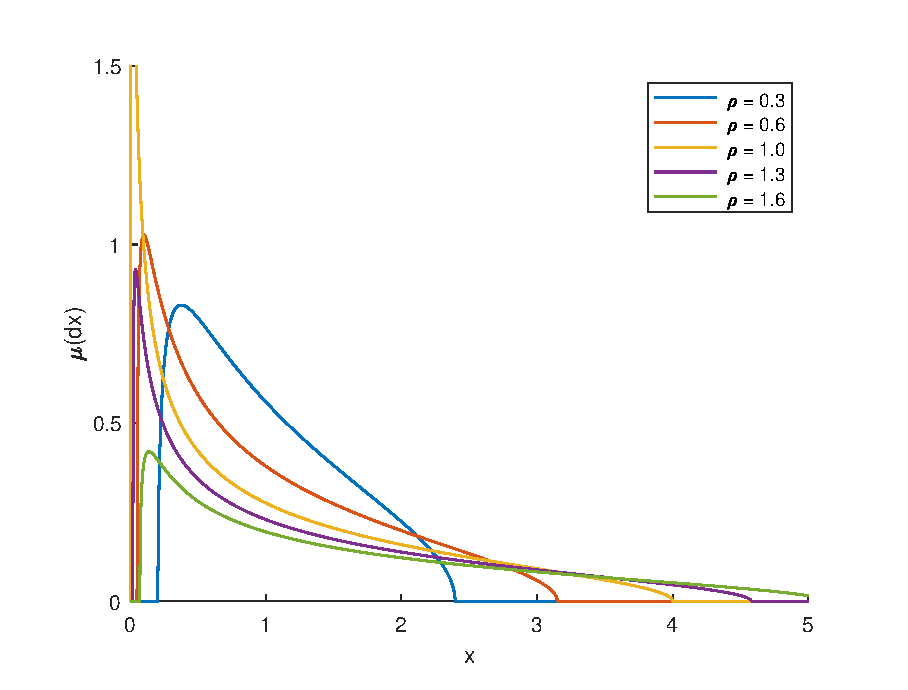
\includegraphics[width=\textwidth]{random-matrix-theory/figures/marchenko-pastur-distribution.eps}
        \caption{The Marčenko-Pastur distribution for $\rho=0.3,0.6,1,1.3,1.6$}
    \end{subfigure}
    \begin{subfigure}{.45\linewidth}
        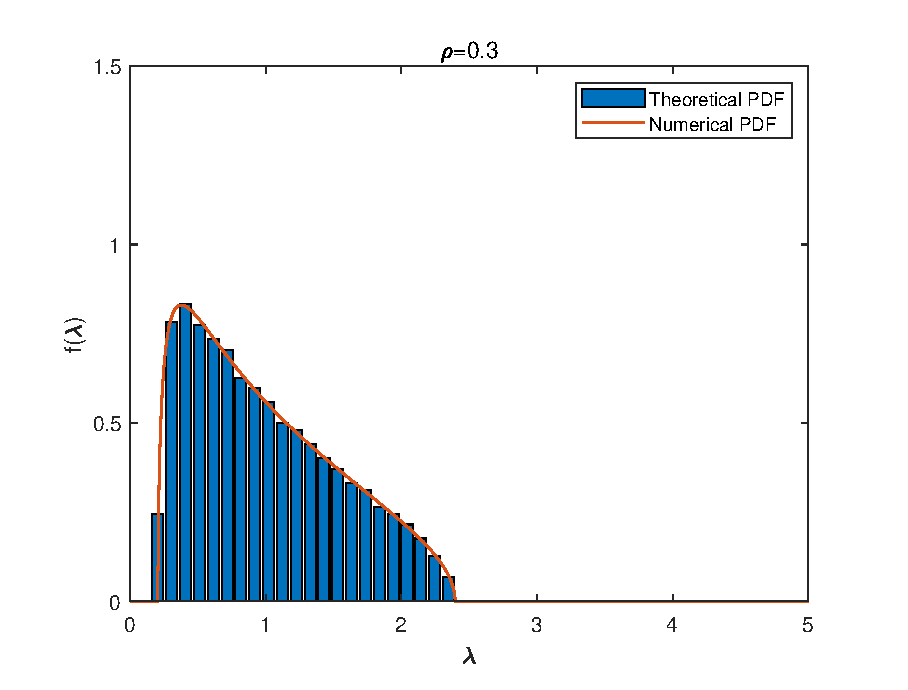
\includegraphics[width=\textwidth]{random-matrix-theory/figures/marchenko-pastur-theorem-simulation.eps}
        \caption{Simulation Results of the Marčenko-Pastur Theorem when $\rho=0.3$}
    \end{subfigure}
    \caption{Illustrations of the Marčenko-Pastur Theorem}
\end{figure}

\begin{proof}
    (Intuitive Proof) Suppose $\overline{\mathbf{Q}}(z)=\mathbf{F}(z)^{-1}$ for some matrix $\mathbf{F}(z)$. To prove $\overline{\mathbf{Q}}(z)$ to be a deterministic equivalent for $\mathbf{Q}(z)$, particularly,
    \begin{equation*}
        \frac{1}{n}\operatorname{tr}\mathbf{A}(\mathbf{Q}(z)-\overline{\mathbf{Q}}(z))\rightarrow 0\quad\text{a.s.}
    \end{equation*}
    where $\mathbf{A}$ is arbitrary, deterministic, and such that $\|\mathbf{A}\|=1$. By Lemma \ref{lem:resolvent-identity}, we have
    \begin{equation*}
        \begin{aligned}
            \mathbf{Q}(z)-\overline{\mathbf{Q}}(z)= & \mathbf{Q}(z)\left(\mathbf{F}(z)+z\mathbf{I}_{n}-\widehat{\boldsymbol{\Sigma}}\right) \overline{\mathbf{Q}}(z)                                         \\
            =                                       & \mathbf{Q}(z)\left(\mathbf{F}(z)+z\mathbf{I}_{n}-\frac{1}{m_{n}}\sum_{i=1}^{m_{n}}\mathbf{X}_{i}\mathbf{X}_{i}^{\prime}\right)\overline{\mathbf{Q}}(z)
        \end{aligned}
    \end{equation*}
    Thus, we turn to prove that,
    \begin{equation*}
        \frac{1}{n}\operatorname{tr}\left[\left(\mathbf{F}(z)+z\mathbf{I}_{n}\right)\overline{\mathbf{Q}}(z)\mathbf{A}\mathbf{Q}(z)\right]-\frac{1}{n}\cdot\frac{1}{m_{n}}\sum_{i=1}^{m_{n}}\mathbf{X}_{i}^{\prime}\overline{\mathbf{Q}}(z)\mathbf{A}\mathbf{Q}(z)\mathbf{X}_{i}\rightarrow 0\quad\text{a.s.}
    \end{equation*}
    By Lemma \ref{lem:sherman-morrison}, we have
    \begin{equation*}
        \mathbf{Q}(z)\mathbf{X}_{i}=\frac{\mathbf{Q}_{-i}(z)\mathbf{X}_{i}}{1+\frac{1}{m_{n}}\mathbf{X}_{i}^{\prime}\mathbf{Q}_{-i}(z)\mathbf{X}_{i}}
    \end{equation*}
    where
    \begin{equation*}
        \mathbf{Q}_{-i}(z)=\left(\frac{1}{m_{n}}\sum_{j\neq i}\mathbf{X}_{j}\mathbf{X}_{j}^{\prime}-z\mathbf{I}_{n}\right)^{-1}
    \end{equation*}
    is independent of $\mathbf{X}_{i}$. By Lemma \ref{lem:quadratic-form-close-to-the-trace}, we have
    \begin{equation*}
        \frac{1}{n}\mathbf{X}_{i}^{\prime}\overline{\mathbf{Q}}(z)\mathbf{A}\mathbf{Q}(z)\mathbf{X}_{i}=\frac{\frac{1}{n}\mathbf{X}_{i}^{\prime}\overline{\mathbf{Q}}(z)\mathbf{A}\mathbf{Q}_{-i}(z)\mathbf{X}_{i}}{1+\frac{1}{m_{n}}\mathbf{X}_{i}^{\prime}\mathbf{Q}_{-i}(z)\mathbf{X}_{i}}\simeq\frac{\frac{1}{n}\operatorname{tr}\left[\overline{\mathbf{Q}}(z)\mathbf{A}\mathbf{Q}_{-i}(z)\right]}{1+\frac{1}{m_{n}}\operatorname{tr}\left[\mathbf{Q}_{-i}(z)\right]}
    \end{equation*}
    Hence, we need to prove the approximation that
    \begin{equation*}
        \frac{1}{n}\operatorname{tr}\left[\left(\mathbf{F}(z)+z\mathbf{I}_{n}\right)\overline{\mathbf{Q}}(z)\mathbf{A}\mathbf{Q}(z)\right]\simeq\frac{\frac{1}{n}\operatorname{tr}\left[\overline{\mathbf{Q}}(z)\mathbf{A}\mathbf{Q}(z)\right]}{1+\frac{1}{m_{n}}\operatorname{tr}\left[\mathbf{Q}(z)\right]}
    \end{equation*}
    If $\mathbf{F}(z)$ exist, for the approximation above to hold, $\mathbf{F}(z)$ must be of the type
    \begin{equation*}
        \mathbf{F}(z)\simeq\left(-z+\frac{1}{1+\frac{1}{m_{n}}\operatorname{tr}\mathbf{Q}(z)}\right)\mathbf{I}_{n}
    \end{equation*}
    By Equation \ref{eq:relation-between-empirical-spectral-measures-stieltjes-transform-and-its-resolvent}, we have,
    \begin{equation*}
        m(z)\equiv\frac{1}{n}\operatorname{tr}\left[\overline{\mathbf{Q}}(z)\right]=\frac{1}{n}\operatorname{tr}\left[\mathbf{F}(z)^{-1}\right]
    \end{equation*}
    taking $\mathbf{A}=\mathbf{I}_{n}$, we have
    \begin{equation*}
        \frac{1}{n}\operatorname{tr}\left[\mathbf{Q}(z)\right]\simeq\frac{1}{n}\operatorname{tr}\left[\overline{\mathbf{Q}}(z)\right]=m(z)=\frac{1}{-z+\frac{1}{1+\frac{n}{m_{n}}\frac{1}{n}\operatorname{tr}\left[\mathbf{Q}(z)\right]}}\simeq\frac{1}{-z+\frac{1}{1+\rho m(z)}}
    \end{equation*}
    As $n,m_{n}\rightarrow\infty$, $m(z)$ is solution to
    \begin{equation*}
        m(z)=\frac{1}{-z+\frac{1}{1+\rho m(z)}}
    \end{equation*}
    or equivalently
    \begin{equation*}
        z\rho m^{2}(z)-(1-\rho-z)m(z)+1=0
    \end{equation*}
    This equation has two solutions defined via the two values of the complex square root function. Let
    \begin{equation*}
        z=r\mathrm{e}^{\imath\theta}\text{ where }r\geq 0,\theta\in[0,2\pi)\Rightarrow\sqrt{z}\in\left\{\pm\sqrt{r}\mathrm{e}^{\imath\theta/2}\right\}
    \end{equation*}
    and we can conclude that
    \begin{equation*}
        m(z)=\frac{1-\rho-z}{2\rho z}+\frac{\sqrt{\left((1+\sqrt{\rho})^{2}-z\right)\left((1-\sqrt{\rho})^{2}-z\right)}}{2\rho z}
    \end{equation*}
    only one of which is such that $\Im[z]\Im[m(z)]>0$ as imposed by the definition of Stieltjes transforms. By the inverse Stieltjes transform theorem, Theorem \ref{thm:inverse-stieltjes-transform}, we find that $m(z)$ is the Stieltjes transform of the measure $\mu$ with
    \begin{equation*}
        \mu([a,b])=\frac{1}{\pi}\lim_{\epsilon\downarrow 0}\int_{a}^{b}\Im[m(x+\imath\epsilon)]\,\mathrm{d}x
    \end{equation*}
    for all continuity points $a,b\in\mathbb{R}$ of $\mu$. This term under the square root in $m(z)$ being negative only in the set
    \begin{equation*}
        \left[(1-\sqrt{\rho})^{2},(1+\sqrt{\rho})^{2}\right]
    \end{equation*}
    (and thus of non-real square root), the latter defines the support of the continuous part of the measure $\mu$ with density
    \begin{equation*}
        \frac{\sqrt{\left((1+\sqrt{\rho})^{2}-x\right)\left(x-(1-\sqrt{\rho})^{2}\right)}}{2\rho\pi x}
    \end{equation*}
    at point $x$ in the set. The case $x=0$ brings a discontinuity in $\mu$ with weight equal to
    \begin{equation*}
        \mu(\{0\})=-\lim_{y\downarrow 0}\imath ym(\imath y)=\frac{\rho-1}{2\rho}\pm\frac{\rho-1}{2\rho}
    \end{equation*}
    where the sign is established by a second order development of $z m(z)$ in the neighborhood of zero: that is, "+" for $c>1$ inducing a mass $1-1/\rho$ for $p>n$, or "-" for $c<1$ in which case $\mu(\{0\})=0$ and $\mu$ has no mass at zero.
\end{proof}

\begin{remark}
    The asymptotic phenomenon holds not only in the Gaussian case, which also holds
    \begin{enumerate}
        \item if $\left(x_{i}\right)_{1\leq i\leq n}$ are i.i.d. with finite second moment.
        \item if $\mathbf{X}$ is isotropic and log-concave\footnote{A probability measure $\mu$ on $\mathbb{R}^{n}$ with density $\varphi$ is log-concave when $\varphi=e^{-V}$ with $V$ convex.} random vector.
    \end{enumerate}
\end{remark}

\section{Limits of Extreme Eigenvalues}

The weak convergence in Theorem \ref{thm:marcenko-pastur-theorem} does not provide much information at the edge on the behavior of the extremal atoms, and what one can actually extract is that
\begin{equation}
    \limsup_{n\rightarrow\infty}\lambda_{\min}\left(\widehat{\boldsymbol{\Sigma}}\right)\leq(1-\sqrt{\rho})^{2}\leq(1+\sqrt{\rho})^{2}\leq\liminf_{n\rightarrow\infty}\lambda_{\max}\left(\widehat{\boldsymbol{\Sigma}}\right)\quad\text{ a.s.}
\end{equation}
where the first inequality is considered only in the case where $m_{n}\geq n$.

The weak convergence above does not provide much information at the edge on the behavior of the extremal atoms. Now, we have more exact result, that if $\left(X_{n,k}\right)_{n\geq 1,1\leq k\leq n}$ are i.i.d. with finite fourth moment then,
\begin{equation} \label{eq:limits-of-extreme-eigenvalues-of-sample-covariance-matrices}
    (1-\sqrt{\rho})^{2}=\lim_{n\rightarrow\infty}\lambda_{\min}\left(\widehat{\boldsymbol{\Sigma}}\right)\leq\lim_{n\rightarrow\infty}\lambda_{\max}\left(\widehat{\boldsymbol{\Sigma}}\right)=(1+\sqrt{\rho})^{2}\quad\text{ a.s.}
\end{equation}
where the first inequality is considered only in the case where $m_{n}\geq n$.

\begin{remark}
    The convergence of the smallest eigenvalue in the left hand side of (\ref{eq:limits-of-extreme-eigenvalues-of-sample-covariance-matrices}) holds if $\left(x_{i}\right)_{1\leq i\leq n}$ are i.i.d. with finite second moment.
\end{remark}

\begin{theorem}
    If $\bar{\rho}<1$ (in particular $m_{n}>n$ for $n\gg 1$ ) and if the centered isotropic random vector $\mathbf{X}$ is log-concave or if $\left(x_{i}\right)_{1\leq i\leq n}$ are i.i.d. then
    \begin{equation}
        \liminf_{n\rightarrow\infty}\frac{E\left(\lambda_{\min}\left(\mathbf{A}_{n}\right)\right)}{\left(\sqrt{m_{n}}-\sqrt{n}\right)^{2}}\geq 1
    \end{equation}
    If additionally $\lim_{n\rightarrow\infty}\frac{n}{m_{n}}=\rho$ with $\rho \in(0,1)$, in other words $\underline{\rho}=\bar{\rho}\in(0,1)$, then
    \begin{equation}
        \lambda_{\min}\left(\widehat{\boldsymbol{\Sigma}}_{n}\right)\stackrel{p}{\longrightarrow}(1-\sqrt{\rho})^{2}\quad\text{ as }n\rightarrow\infty
    \end{equation}
\end{theorem}

\begin{proof}

\end{proof}

\begin{theorem}
    If the centered isotropic random vector $\mathbf{X}$ is log-concave or if $\left(x_{i}\right)_{1\leq i\leq n}$ are i.i.d. with finite 4-th moment then
    \begin{equation}
        \limsup_{n\rightarrow\infty}\frac{E\left(\lambda_{\max}\left(\mathbf{A}_{n}\right)\right)}{\left(\sqrt{m_{n}}+\sqrt{n}\right)^{2}}\leq 1
    \end{equation}
    If additionally $\lim_{n\rightarrow\infty}\frac{n}{m_{n}}=\rho$ with $\rho \in(0,1)$, in other words $\underline{\rho}=\bar{\rho}\in(0,1)$, then
    \begin{equation}
        \lambda_{\max}\left(\widehat{\boldsymbol{\Sigma}}_{n}\right)\stackrel{p}{\longrightarrow}(1+\sqrt{\rho})^{2}\quad\text{ as }n\rightarrow\infty
    \end{equation}
\end{theorem}

\begin{proof}

\end{proof}

% Statistics
\part{Statistics Inference}
\chapter{Statistical Theory}

\section{Populations and Samples}

\section{Statistics}

\subsection{Sufficient Statistics}

\begin{definition}[Sufficient Statistics]
    A statistic $T$ is said to be sufficient for $X$, or for the family $\mathcal{P}=\left\{P_{\theta}, \theta \in \Omega\right\}$ of possible distributions of $X$, or for $\theta$, if the conditional distribution of $X$ given $T=t$ is independent of $\theta$ for all $t$.
\end{definition}

\begin{theorem}[Fisher–Neyman Factorization Theorem]
    If the probability density function is $p_{\theta}(x)$, then $T$ is sufficient for $\theta$ if and only if nonnegative functions $g$ and $h$ can be found such that
    \begin{equation*}
        p_{\theta}(x)=h(x)g_{\theta}[T(x)].
    \end{equation*}
\end{theorem}

\begin{proof}

\end{proof}

\subsection{Complete Statistics}

\begin{definition}[Complete Statistics]
    A statistic $T$ is said to be complete, if $Eg(T)=0$ for all $\theta$ and some function $g$ implies that $P(g(T)=0\mid\theta)=1$ for all $\theta$.
\end{definition}

\section{Estimators}

\begin{definition}[Estimator] \label{def:estimator}
    An estimator is a real-valued function defined over the sample space, that is
    \begin{equation}
        \delta:\textbf{X}\rightarrow\mathbb{R}.
    \end{equation}
    It is used to estimate an estimand, $\theta$, a real-valued function of the parameter.
\end{definition}

\subsection*{Unbiasedness}

\begin{definition}[Unbiasedness]
    An estimator $\hat{\theta}$ of $\theta$ is unbiased if
    \begin{equation}
        E\hat{\theta}=\theta,\quad\forall\theta\in\Theta.
    \end{equation}
\end{definition}

\begin{remark}
    \begin{itemize}
        \item Unbiased estimators of $\theta$ may not exist.
        \item
    \end{itemize}
\end{remark}

\begin{example}[Nonexistence of Unbiased Estimator]

\end{example}

\subsection*{Consistency}

\begin{definition}[Consistency]
    An estimator $\hat{\theta}_n$ of $\theta$ is consistent if
    \begin{equation}
        \lim_{n\rightarrow\infty}P\left(\left|\hat{\theta}_n-\theta\right|>\varepsilon\right)=0,\quad\forall\varepsilon>0,
    \end{equation}
    that is,
    \begin{equation}
        \hat{\theta}_{n}\stackrel{p}{\rightarrow}\theta.
    \end{equation}
\end{definition}

\begin{example}[Consistency of Sample Moments]
    
\end{example}

\begin{remark}
    \begin{enumerate}
        \item Unbiased But Consistent
        \item Biased But Not Consistent
    \end{enumerate}
\end{remark}

\subsection*{Asymptotic Normality}

\begin{definition}[Asymptotic Normality]
    An estimator $\hat{\theta}_n$ of $\theta$ is asymptotic normality if
    \begin{equation}
        \sqrt{n}\left(\hat{\theta}-\theta\right)\stackrel{d}{\rightarrow}N\left(0,\sigma_{\theta}^{2}\right).
    \end{equation}
\end{definition}

\subsection*{Efficiency}

\begin{definition}[Efficiency]

\end{definition}

\subsection*{Robustness}

\begin{definition}[Robustness]

\end{definition}

\chapter{Frequentist Inference}

\section{Point Estimation}

\subsection{Minimum-Variance Unbiased Estimator}

\begin{definition}[UMVU Estimators]
    An unbiased estimator $\delta(\textbf{X})$ of $g(\theta)$ is the uniform minimum variance unbiased (UMVU) estimator of $g(\theta)$ if
    \begin{equation}
        \text{Var}_{\theta}\delta(\textbf{X})\leq\text{Var}_{\theta}\delta'(\textbf{X}),\quad\forall\theta\in\Theta,
    \end{equation}
    where $\delta'(\textbf{X})$ is any other unbiased estimator of $g(\theta)$.
\end{definition}

\begin{remark}
    If there exists an unbiased estimator of $g$, the estimand $g$ will be called $U$-estimable.
\end{remark}

\begin{enumerate}
    \item If $T(\textbf{X})$ is a complete sufficient statistic, estimator $\delta(\textbf{X})$ that only depends on $T(\textbf{X})$, then for any $U$-estimable function $g(\theta)$ with
          \begin{equation}
              E_{\theta}\delta(T(\textbf{X}))=g(\theta),\quad\forall\theta\in\Theta,
          \end{equation}
          hence, $\delta(T(\textbf{X}))$ is the unique UMVU estimator of $g(\theta)$.
    \item If $T(\textbf{X})$ is a complete sufficient statistic and $\delta({\textbf{X}})$ is any unbiased estimator of $g(\theta)$, then the UMVU estimator of $g(\theta)$ can be obtained by
          \begin{equation}
              E\left[\delta(\textbf{X})\mid T(\textbf{X})\right].
          \end{equation}
\end{enumerate}

\begin{example}[Estimating Polynomials of a Normal Variance]
    Let $X_{1},\ldots,X_{n}$ be distributed with joint density
    \begin{equation}
        \frac{1}{(\sqrt{2\pi}\sigma)^{n}}\exp\left[-\frac{1}{2\sigma^{2}}\sum\left(x_{i}-\xi\right)^{2}\right].
    \end{equation}
    Discussing the UMVU estimators of $\xi^r$, $\sigma^r$, $\xi/\sigma$.
\end{example}

\begin{proof}
    \begin{enumerate}
        \item \textbf{$\sigma$ is known}:

              Since $\bar{X}=\frac{1}{n}\sum_{i=1}^{n}X_i$ is the complete sufficient statistic of $X_i$, and
              \begin{equation*}
                  E(\bar{X})=\xi,
              \end{equation*}
              then the UMVU estimator of $\xi$ is $\bar{X}$.

              Therefore, the UMVU estimator of $\xi^r$ is $\bar{X}^r$ and the UMVU estimator of $\xi/\sigma$ is $\bar{X}/\sigma$.

        \item \textbf{$\xi$ is known}:

              Since $s^r=\sum\left(x_{i}-\xi\right)^r$ is the complete sufficient statistic of $X_i$.

              Assume
              \begin{equation*}
                  E\left[\frac{s^r}{\sigma^r}\right]=\frac{1}{K_{n,r}},
              \end{equation*}
              where $K_{n,r}$ is a constant depends on $n,r$.

              Since $s^2/\sigma^2\sim\text{Ga}(n/2,1/2)=\chi^2(n)$, then
              \begin{equation*}
                  E\left[\frac{s^r}{\sigma^r}\right]=E\left[\left(\frac{s^2}{\sigma^2}\right)^{\frac{r}{2}}\right]=\int_{0}^{\infty}x^{\frac{r}{2}}\frac{1}{2^{\frac{n}{2}}\Gamma(\frac{n}{2})}x^{\frac{n}{2}-1}e^{-\frac{x}{2}}\mathrm{d}x=\frac{\Gamma\left(\frac{n+r}{2}\right)}{\Gamma(\frac{n}{2})}\cdot 2^{\frac{r}{2}}.
              \end{equation*}
              therefore,
              \begin{equation*}
                  K_{n,r}=\frac{\Gamma(\frac{n}{2})}{2^{\frac{r}{2}}\cdot\Gamma\left(\frac{n+r}{2}\right)}.
              \end{equation*}

              Hence,
              \begin{equation*}
                  E\left[s^rK_{n,r}\right]=\sigma^r \text{ and } E[\xi s^{-1}K_{n,-1}]=\xi/\sigma,
              \end{equation*}
              which means the UMVU estimator of $\sigma^r$ is $s^rK_{n,r}$ and the UMVU estimator of $\xi/\sigma$ is $\xi s^{-1}K_{n,-1}$.

        \item \textbf{Both $\xi$ and $\sigma$ is unknown}:

              Since $(\bar{X},s_x^r)$ are the complete sufficient statistic of $X_i$, where $s_x^2=\sum\left(x_{i}-\bar{X}\right)^r$.

              Since $s_x^2/\sigma^2\sim\chi^2(n-1)$, then
              \begin{equation*}
                  E\left[\frac{s_x^r}{\sigma^r}\right]=\frac{1}{K_{n-1,r}}.
              \end{equation*}

              Hence,
              \begin{equation*}
                  E\left[s_x^rK_{n-1,r}\right]=\sigma^r,
              \end{equation*}
              which means the UMVU estimator of $\sigma^r$ is $s_x^rK_{n-1,r}$,
              and
              \begin{equation*}
                  E(\bar{X}^r)=\xi^r,
              \end{equation*}
              which means the UMVU estimator of $\xi^r$ is $\bar{X}^r$.

              Since $\bar{X}$ and $s_x^r$ are independent, then
              \begin{equation*}
                  E[\bar{X}s_x^{-1}K_{n-1,-1}]=\xi/\sigma
              \end{equation*}
              which means the UMVU estimator of $\xi/\sigma$ is $\bar{X}s_x^{-1}K_{n-1,-1}$.
    \end{enumerate}
\end{proof}

\begin{example}[]
    Let $X_{1},\ldots,X_{n}$ be i.i.d sample from $U\left(\theta_1-\theta_2,\theta_1+\theta_2\right)$, where $\theta_1\in\mathbb{R},\theta_2\in\mathbb{R}^+$. Discussing the UMVU estimators of $\theta_1,\theta_2$.
\end{example}

\begin{proof}
    Let $X_{(i)}$ be the i-th order statistic of $X_i$, then $\left(X_{(1)},X_{(n)}\right)$ is the complete and sufficient statistic for $(\theta_1,\theta_2)$. Thus it suffices to find a function $\left(X_{(1)},X_{(n)}\right)$, which is unbiased of $(\theta_1,\theta_2)$.

    Let
    \begin{equation*}
        Y_i=\frac{X_i-(\theta_1-\theta_2)}{2\theta_2}\sim U(0,1),
    \end{equation*}
    and
    \begin{equation*}
        Y_{(i)}=\frac{X_{(i)}-(\theta_1-\theta_2)}{2\theta_2},
    \end{equation*}
    be the i-th order statistic of $Y_i$, then we got
    \begin{equation*}
        \begin{aligned}
            E[X_{(1)}] & = 2\theta_2E[Y_{(1)}]+(\theta_1-\theta_2)                           \\
                       & = 2\theta_2\int_{0}^{1}ny(1-y)^{n-1}\mathrm{d}y+(\theta_1-\theta_2) \\
                       & = \theta_1-\frac{3n+1}{n+1}\theta_2                                 \\
            E[X_{(n)}] & = 2\theta_2E[Y_{(n)}]+(\theta_1-\theta_2)                           \\
                       & = 2\theta_2\int_{0}^{1}ny^{n}\mathrm{d}y+(\theta_1-\theta_2)        \\
                       & = \theta_1+\frac{n-1}{n+1}\theta_2                                  \\
        \end{aligned}.
    \end{equation*}

    Thus,
    \begin{equation*}
        \begin{aligned}
            \theta_1 & = E\left[\frac{n-1}{4n}X_{(1)}+\frac{3n+1}{4n}X_{(n)}\right], \\
            \theta_2 & = E\left[-\frac{n+1}{4n}X_{(1)}+\frac{n+1}{4n}X_{(n)}\right], \\
        \end{aligned}
    \end{equation*}
    which means the UMVU estimator is
    \begin{equation*}
        \hat{\theta_1}=\frac{n-1}{4n}X_{(1)}+\frac{3n+1}{4n}X_{(n)},\quad\hat{\theta_2}=-\frac{n+1}{4n}X_{(1)}+\frac{n+1}{4n}X_{(n)}.
    \end{equation*}
\end{proof}

\subsection{Maximum Likelihood Estimator}

Suppose that $\textbf{X}_{n}=\left(X_{1},\ldots,X_{n}\right)$, where the $X_{i}$ are i.i.d. with common density $p\left(x;\theta_{0}\right)\in\mathcal{P}=\{p(x;\theta):\theta\in\Theta\}$.

We assume that

\begin{quotation}
    $\theta_{0}$ is identified in the sense that if $\theta\neq\theta_{0}$ and $\theta\in\Theta$, then $p(x;\theta)\neq p\left(x;\theta_{0}\right)$ with respect to the dominating measure $\mu$.
\end{quotation}

For fixed $\theta\in\Theta$, the joint density of $\textbf{X}_{n}$ is equal to the product of the individual densities, i.e.,

\begin{equation}
    p\left(\textbf{X}_{n};\theta\right)=\prod_{i=1}^{n} p\left(x_{i};\theta\right).
\end{equation}

The maximum likelihood estimate for observed $\textbf{X}_{n}$ is the value $\theta\in\Theta$ which maximizes $L\left(\theta;X_{n}\right):=p\left(\textbf{X}_{n};\theta\right)$, i.e.,

\begin{equation}
    \hat{\theta}\left(\textbf{X}_{n}\right)=\max_{\theta\in\Theta}L\left(\theta;X_{n}\right).
\end{equation}

Equivalently, the MLE can be taken to be the maximum of the standardized log-likelihood,

\begin{equation}
    \frac{l\left(\theta;\textbf{X}_{n}\right)}{n}=\frac{\log L\left(\theta;\textbf{X}_{n}\right)}{n}=\frac{1}{n}\sum_{i=1}^{n}\log p\left(X_{i};\theta\right)=\frac{1}{n}\sum_{i=1}^{n}l\left(\theta;X_{i}\right).
\end{equation}

Define
\begin{equation}
    \begin{gathered}
        Q\left(\theta;\textbf{X}_{n}\right):=\frac{1}{n}\sum_{i=1}^{n}l\left(\theta;X_{i}\right), \\
        \hat{\theta}\left(\textbf{X}_{n}\right):=\max_{\theta\in\Theta}Q\left(\theta;\textbf{X}_{n}\right). \\
    \end{gathered}
\end{equation}

\subsubsection{Consistency of MLE}

By the Weak Law of Large Numbers (Theorem \ref{thm:WLLN}), we can get,

\begin{equation}
    \frac{1}{n}\sum^{n}l\left(\theta;X_{i}\right)\stackrel{p}{\rightarrow}E\left[l(\theta;X)\right].
\end{equation}

Suppose $Q_{0}(\theta)=E\left[l(\theta;X)\right]$, then we will show that $Q_{0}(\theta)$ is maximized at $\theta_{0}$ (i.e., the truth).

\begin{lemma}
    If $\theta_{0}$ is identified and $E_{\theta_{0}}\left[|\log p(X;\theta)|\right]<\infty,\forall\theta\in\Theta$, then $Q_{0}(\theta)$ is uniquely maximized at $\theta=\theta_{0}$.
\end{lemma}

\begin{proof}

\end{proof}

\begin{theorem}[Consistency of MLE]
    Suppose that $Q\left(\theta;\textbf{X}_{n}\right)$ is continuous in $\theta$ and there exists a function $Q_{0}(\theta)$ such that
    \begin{enumerate}
        \item $Q_{0}(\theta)$ is uniquely maximized at $\theta_{0}$.
        \item $\Theta$ is compact.
        \item $Q_{0}(\theta)$ is continuous in $\theta$.
        \item $Q\left(\theta;\textbf{X}_{n}\right)$ converges uniformly in probability to $Q_{0}(\theta)$.
    \end{enumerate}
    then
    \begin{equation}
        \hat{\theta}\left(\textbf{X}_{n}\right)\stackrel{p}{\rightarrow}\theta_{0}.
    \end{equation}
\end{theorem}

\begin{proof}
    $\forall\varepsilon>0$, let
    \begin{equation*}
        \Theta(\epsilon)=\left\{\theta:\left\|\theta-\theta_{0}\right\|<\epsilon\right\}.
    \end{equation*}

    Since $\Theta(\epsilon)$ is an open set, then $\Theta\cap\Theta(\epsilon)^{C}$ is a compact set (Assumption 2).

    Since $Q_{0}(\theta)$ is a continuous function (Assumption 3), then
    \begin{equation*}
        \theta^{*}:=\sup_{\theta\in\Theta\cap \Theta(\epsilon)^{C}}\left\{Q_{0}(\theta)\right\}
    \end{equation*}
    is a achieved for a $\theta$ in the compact set.

    Since $\theta_{0}$ is the unique maximized, let
    \begin{equation*}
        Q_{0}\left(\theta_{0}\right)-Q_{0}\left(\theta^{*}\right)=\delta>0.
    \end{equation*}

    \begin{enumerate}
        \item For $\theta\in\Theta\cap\Theta(\epsilon)^{C}$. Let $A_n=\left\{\sup_{\theta\in\Theta\cap\Theta(\epsilon)^{C}}\left|Q\left(\theta;\textbf{X}_{n}\right)-Q_{0}(\theta)\right|<\frac{\delta}{2}\right\}$, then
              \begin{equation*}
                  \begin{aligned}
                      A_{n}\Rightarrow Q\left(\theta;\textbf{X}_{n}\right) & <Q_{0}(\theta)+\frac{\delta}{2}                    \\
                                                                           & \leq Q_{0}\left(\theta^{*}\right)+\frac{\delta}{2} \\
                                                                           & = Q_{0}\left(\theta_{0}\right)-\frac{\delta}{2}
                  \end{aligned}
              \end{equation*}
        \item For $\theta\in\Theta(\epsilon)$. Let $B_n=\left\{\sup_{\theta\in\Theta(\epsilon)}\left|Q\left(\theta;\boldsymbol{X}_{n}\right)-Q_{0}(\theta)\right|<\frac{\delta}{2}\right\}$, then
              \begin{equation*}
                  B_{n}\Rightarrow Q\left(\theta;\boldsymbol{X}_{n}\right)>Q_{0}(\theta)-\frac{\delta}{2},\forall\theta\in\Theta(\epsilon)
              \end{equation*}
              By Assumption 1,
              \begin{equation*}
                  Q\left(\theta_{0};\boldsymbol{X}_{n}\right)>Q_{0}\left(\theta_{0}\right)-\frac{\delta}{2}
              \end{equation*}
    \end{enumerate}

    If both $A_{n}$ and $B_{n}$ hold, then
    \begin{equation*}
        \hat{\theta}\in\Theta(\epsilon).
    \end{equation*}

    By Assumption 4, we can concluded that $P\left(A_{n}\cap B_{n}\right)\rightarrow 1$, so
    \begin{equation*}
        P(\hat{\theta}\in\Theta(\epsilon))\rightarrow 1,
    \end{equation*}
    which means,
    \begin{equation*}
        \hat{\theta}\left(\textbf{X}_{n}\right)\stackrel{p}{\rightarrow}\theta_{0}.
    \end{equation*}
\end{proof}

\subsubsection{Asymptotic Normality of MLE}

\subsubsection{Efficiency of MLE}

\chapter{Specific Tests}

\section{Goodness of Fit}

\subsection{Likelihood-Ratio Test}


\chapter{Bayesian Inference}

\section{Bayes Estimator}

We shall look for some estimators that make the risk function $R\left(\theta,\delta\right)$ small in some overall sense. There are two ways to solve it: minimize the average risk, and minimize the maximum risk.

This chapter will discuss the first method, also known as, Bayes Estimator.

\begin{definition}[Bayes Estimator] \label{def:bayes-estimator}
	The Bayes Estimator $\delta$ with respect to $\Lambda$ is minimizing the Bayes Risk of $\delta$
	\begin{equation}
		r\left(\Lambda, \delta\right)=\int R\left(\theta, \delta\right) \dif \Lambda\left(\theta\right)
	\end{equation}
	where $\Lambda$ is the probability distribution.
\end{definition}

In Bayesian arguments, it is important to keep track of which variables are being conditioned. Hence, the notations are as follows:
\begin{itemize}
	\item The density of $X$ will be denoted by $X \sim f\left(x \mid \theta\right)$.
	\item The prior distribution will be denoted by $\Pi \sim \pi\left(\theta \mid \lambda\right)$ or $\Lambda \sim \gamma\left(\lambda\right)$, where $\lambda$ is another parameter (sometimes called a hyperparameter).
	\item The posterior distribution, which calculates the conditional distributions as that of $\theta$ given $x$ and $\lambda$, or $\lambda$ given $x$, which is denoted by $\Pi \sim \pi\left(\theta \mid x, \lambda\right)$ or $\Lambda \sim \gamma\left(\lambda \mid x\right)$, that is
	      \begin{equation}
		      \pi\left(\theta \mid x, \lambda\right) = \frac{f\left(x \mid \theta\right) \pi\left(\theta \mid \lambda\right)}{m\left(x \mid \lambda\right)},
	      \end{equation}
	      where marginal distributions $m\left(x \mid \lambda\right) = \int f\left(x \mid \theta\right) \pi\left(\theta \mid \lambda\right) \dif \theta$.
\end{itemize}

\begin{theorem} \label{thm:bayes-definition}
	Let $\Theta$ have distribution $\Lambda$, and given $\Theta=\theta$, let $X$ have distribution $P_{\theta}$. Suppose, the following assumptions hold for the problem of estimating $g\left(\Theta\right)$ with non-negative loss function $L\left(\theta,d\right)$,
	\begin{itemize}
		\item There exists an estimator $\delta_0$ with finite risk.
		\item For almost all $x$, there exists a value $\delta_{\Lambda}\left(x\right)$ minimizing
		      \begin{equation}
			      E\{L[\Theta,\delta\left(x\right)] \mid X=x\}.
		      \end{equation}
	\end{itemize}
	Then, $\delta_{\Lambda}\left(x\right)$ is a Bayes Estimator.
\end{theorem}
\begin{remark}
	Improper prior
\end{remark}

\begin{corollary}
	Suppose the assumptions of Theorem~\ref{thm:bayes-definition} hold.
	\begin{enumerate}
		\item If $L\left(\theta,d\right)=[d-g\left(\theta\right)]^2$, then
		      \begin{equation}
			      \delta_{\Lambda}\left(x\right)=E[g\left(\Theta\right) \mid x].
		      \end{equation}
		\item If $L\left(\theta,d\right)=w\left(\theta\right)[d-g\left(\theta\right)]^2$, then
		      \begin{equation}
			      \delta_{\Lambda}\left(x\right)=\frac{E[w\left(\theta\right)g\left(\Theta\right) \mid x]}{E[w\left(\theta\right) \mid x]}.
		      \end{equation}
		\item If $L\left(\theta,d\right)=|d-g\left(\theta\right)|$, then $\delta_\Lambda\left(x\right)$ is any median of the conditional distribution of $\Theta$ given $x$.
		\item If
		      \begin{equation*}
			      L(\theta, d)=\left\{
			      \begin{array}{l}
				      0 \text { when }|d-\theta| \leq c \\
				      1 \text { when }|d-\theta|>c
			      \end{array}
			      \right.,
		      \end{equation*}
		      then $\delta_\Lambda\left(x\right)$ is the midpoint of the interval $I$ of length $2c$ which maxmizes $P\left(\Theta\in I\mid x\right)$.
	\end{enumerate}
\end{corollary}

\begin{proof}

\end{proof}

\begin{theorem}
	Necessary condition for Bayes Estimator
\end{theorem}

Methodologies have been developed to deal with the difficulty which sometimes incorporates frequentist measures to assess the choice of $\Lambda$.

\begin{itemize}
	\item Empirical Bayes.
	\item Hierarchical Bayes.
	\item Robust Bayes.
	\item Objective Bayes.
\end{itemize}

\subsection{Single-Prior Bayes}

The Single-Prior Bayes model in a general form as
\begin{equation}
	\begin{aligned}
		X\mid\theta      & \sim f\left(x\mid\theta\right),         \\
		\Theta\mid\gamma & \sim \pi\left(\theta\mid\lambda\right),
	\end{aligned}
	\label{eq:single-prior-bayes}
\end{equation}
where we assume that the functional form of the prior and the value of $\lambda$ is known (we will write it as $\gamma=\gamma_0)$.

Given a loss function $L\left(\theta,d\right)$, we would then determine the estimator that minimizes
\begin{equation}
	\int L\left(\theta,d\left(x\right)\right)\pi\left(\theta\mid x\right)\dif\theta,
\end{equation}
where $\pi\left(\theta\mid x\right)$ is posterior distribution given by
\begin{equation*}
	\pi\left(\theta\mid x\right)=\frac{f\left(x\mid\theta\right)\pi\left(\theta\mid\gamma_0\right)}{\int f\left(x\mid\theta\right)\pi\left(\theta\mid\gamma_0\right)\dif\theta}.
\end{equation*}

In general, this Bayes estimator under squared error loss is given by
\begin{equation}
	E\left(\Theta\mid x\right) = \frac{\int\theta f\left(x\mid\theta\right)\pi\left(\theta\mid\gamma_0\right)\dif\theta}{\int f\left(x\mid\theta\right)\pi\left(\theta\mid\gamma_0\right)\dif\theta}.
\end{equation}

\begin{example}
	Consider
	\begin{equation*}
		\begin{aligned}
			X_i    & \stackrel{\text{i.i.d}}{\sim}N(\mu,\Gamma^{-1}),\quad i=1,2,\ldots,n \\
			\mu    & \sim N(0,1),                                                         \\
			\Gamma & \sim\text{Gamma}(2,1),
		\end{aligned}
	\end{equation*}
	calculate the Single-Prior Bayes estimator under squared error loss.
\end{example}

\begin{proof}
	\begin{equation*}
		\begin{aligned}
			p\left(\textbf{X}\mid\mu,\Gamma\right) & =\Gamma^n(2\pi)^{-\frac{n}{2}}\exp\left[-2\Gamma^2\sum_{i=1}^{n}(x_i-\mu)^2\right], \\
			p(\mu)                                 & =\frac{1}{\sqrt{2\pi}}\exp\left(-\frac{\mu^2}{2}\right),                            \\
			p(\Gamma)                              & =\frac{1}{\Gamma(2)}\Gamma\exp\left(-\Gamma\right).
		\end{aligned}
	\end{equation*}

	Therefore,
	\begin{equation*}
		h\left(\textbf{X},\mu,\Gamma\right)=C\Gamma^n\exp\left[-2\Gamma^2\sum_{i=1}^{n}(x_i-\mu)^2\right]\exp\left(-\frac{\mu^2}{2}\right)\Gamma\exp\left(-\Gamma\right),
	\end{equation*}
	where $C=\frac{(2\pi)^{-\frac{n+1}{2}}}{\Gamma(2)}$.

	For $\mu$, we have
	\begin{equation*}
		\pi\left(\mu\mid\textbf{X},\Gamma\right)=\frac{h\left(\textbf{X},\mu,\Gamma\right)}{p(\mu\mid\textbf{X})}
	\end{equation*}
\end{proof}

For exponential families

\begin{theorem}

\end{theorem}

\subsection{Hierarchical Bayes}

In a Hierarchical Bayes model, rather than specifying the prior distribution as a single function, we specify it in a \textbf{hierarchy}. Thus, the Hierarchical Bayes model in a general form as
\begin{equation}
	\begin{aligned}
		X\mid\theta      & \sim f\left(x\mid\theta\right),         \\
		\Theta\mid\gamma & \sim \pi\left(\theta\mid\lambda\right), \\
		\Gamma           & \sim \psi\left(\gamma\right),
	\end{aligned}
	\label{eq:hierarchical-bayes}
\end{equation}
where we assume that $\psi\left(\cdot\right)$ is known and not dependent on any other unknown hyperparameters.

\begin{remark}
	We can continue this hierarchical modeling and add more stages to the model, but this is not then done in practice.
\end{remark}

Given a loss function $L\left(\theta,d\right)$, we would then determine the estimator that minimizes
\begin{equation} \label{eq:hierarchical-bayes-estimator}
	\int L\left(\theta,d\left(x\right)\right)\pi\left(\theta\mid x\right)\dif\theta,
\end{equation}
where $\pi\left(\theta\mid x\right)$ is posterior distribution given by
\begin{equation*}
	\pi\left(\theta\mid x\right)=\frac{\int f\left(x\mid\theta\right)\pi\left(\theta\mid\gamma\right)\psi\left(\gamma\right)\dif\gamma}{\int\int f\left(x\mid\theta\right)\pi\left(\theta\mid\gamma\right)\psi\left(\gamma\right)\dif\theta\dif\gamma}.
\end{equation*}

\begin{remark}
	The posterior distribution can also be written as
	\begin{equation*}
		\pi\left(\theta\mid x\right)=\int\pi\left(\theta\mid x,\gamma\right)\pi\left(\gamma\mid x\right)\dif\gamma,
	\end{equation*}
	where $\pi\left(\gamma\mid x\right)$ is the posterior distribution of $\Gamma$, unconditional on $\theta$. The equation~\ref{eq:hierarchical-bayes-estimator} can be written as
	\begin{equation*}
		\int L\left(\theta,d\left(x\right)\right)\pi\left(\theta\mid x\right)\dif\theta = \int\left[\int L\left(\theta,d\left(x\right)\right)\pi\left(\theta\mid x,\gamma\right)\dif\theta\right]\pi\left(\gamma\mid x\right)\dif\gamma.
	\end{equation*}
	which shows that \textbf{the Hierarchical Bayes estimator can be thought of as a mixture of Single-Prior estimators}.
\end{remark}

\begin{example}[Poisson Hierarchy]
	Consider
	\begin{equation}
		\begin{aligned}
			X_i\mid\lambda & \stackrel{\text{i.i.d}}{\sim} \text{Poisson}\left(\lambda\right),\quad i=1,2\ldots,n \\
			\lambda\mid b  & \sim \text{Gamma}\left(a,b\right), \text{a known},                                   \\
			\frac{1}{b}    & \sim \text{Gamma}\left(k,\tau\right),                                                \\
		\end{aligned}
	\end{equation}
	calculate the Hierarchical Bayes estimator under squared error loss.
\end{example}

\begin{theorem}
	For the Hierarchical Bayes model (\ref{eq:hierarchical-bayes}),
	\begin{equation}
		K\left[\pi\left(\lambda\mid x\right),\psi\left(\lambda\right)\right] < K\left[\pi\left(\theta\mid x\right),\pi\left(\theta\right)\right],
	\end{equation}
	where $K$ is the Kullback-Leibler information for discrimination between two densities.
\end{theorem}

\begin{proof}

\end{proof}

\begin{remark}

\end{remark}

\subsection{Empirical Bayes}

\subsection{Bayes Prediction}

\chapter{Nonparametric Statistics}

\section{Probability Distribution}

\subsection{Cumulative Distribution Function}

Let $X_{1},\ldots,X_{n}\sim F$ where $F(x)=\mathbb{P}(X\leq x)$ is a distribution function on the real line.

\begin{definition}[Empirical Cumulative Distribution Function]
	The empirical cumulative distribution function $\widehat{F}_{n}$ is the CDF that puts mass $1/n$ at each data point $X_{i}$, that,
	\begin{equation}
		\widehat{F}_{n}(x)=\frac{1}{n}\sum_{i=1}^{n}I\left(X_{i}\leq x\right)
	\end{equation}
\end{definition}

\subsection{Probability Density Function}

\subsubsection{Histogram}

\subsubsection{Kernel Density Estimation}

\section{Kernel Methods}

\subsection{Positive Definite Kernels}

\begin{definition}[Positive Definite Kernel]
	Let $\mathcal{X}$ be a set, a function $K:\mathcal{X}\times\mathcal{X}\rightarrow\bbR$ is called a positive definite kernel on $\mathcal{X}$ iff it is
	\begin{enumerate}
		\item symmetric, that is,
		      \begin{equation}
			      K\left(\bfx,\bfx^{\prime}\right)=K\left(\bfx^{\prime},\bfx\right),\quad\forall\bfx,\bfx^{\prime}\in\mathcal{X}
		      \end{equation}
		\item positive definite, that is,
		      \begin{equation}
			      \sum_{i=1}^{n}\sum_{j=1}^{n}c_{i}c_{j}K\left(\bfx_{i},\bfx_{j}\right)\geq 0,
		      \end{equation}
		      holds for any $x_{1},\ldots,x_{n}\in\mathcal{X}$, given $n\in\mathbb{N},c_{1},\ldots,c_{n}\in\bbR$.
	\end{enumerate}
\end{definition}

\subsubsection{Construction of the Reproducing Kernel Hilbert Space}

\begin{theorem}[Morse-Aronszajn's Theorem] \label{thm:morse-aronszajn}
	For any set $\mathcal{X}$, suppose $K:\mathcal{X}\times\mathcal{X}\rightarrow\bbR$ is positive definite, then there is a unique RKHS $\mathcal{H}\subset\bbR^{\mathcal{X}}$ with reproducing kernel $K$.
\end{theorem}

\begin{proof}
	\begin{enumerate}
		\item How to build a valid pre-RKHS $\mathcal{H}_{0}$?

		      Consider the vector space $\mathcal{H}_{0}\subset\mathcal{R}^{\mathcal{X}}$ spanned by the functions $\left\{K\left(\cdot,\bfx\right)\right\}_{\bfx\in\mathcal{X}}$. For any $f,g\in\mathcal{H}_{0}$, suppose
		      \begin{equation*}
			      f=\sum_{i=1}^{m}a_{i}K\left(\cdot,\bfx_{i}\right),\quad g=\sum_{j=1}^{n}b_{j}K\left(\cdot,\mathbf{y}_{j}\right)
		      \end{equation*}
		      and let the inner product of $\mathcal{H}_{0}$ be
		      \begin{equation}
			      \left\langle f,g\right\rangle=\sum_{i=1}^{m}\sum_{j=1}^{n}a_{i}b_{j}K\left(\bfx_{i},\mathbf{y}_{j}\right)
			      \label{eq:definition-pre-rkhs-inner-product}
		      \end{equation}

		      Let $\bfx\in\mathcal{X}$,
		      \begin{equation*}
			      \left\langle f,K\left(\cdot,\bfx\right)\right\rangle_{\mathcal{H}_{0}}=\sum_{i=1}^{m}a_{i} K\left(\bfx,\bfx_{i}\right)=f(\bfx)
			      \label{eq:reproducing-kernel}
		      \end{equation*}

		      And, we also have
		      \begin{equation*}
			      \langle f, g\rangle_{\mathcal{H}_{0}}=\sum_{i=1}^{m} a_{i} g\left(\bfx_{i}\right)=\sum_{j=1}^{n} b_{j} f\left(\mathbf{y}_{j}\right)
		      \end{equation*}

		      Suppose
		      \begin{equation*}
			      f=\sum_{i=1}^{m}a_{i}K\left(\cdot,\bfx_{i}\right),\quad g=\sum_{j=1}^{n}b_{j}K\left(\cdot,\mathbf{y}_{j}\right),\quad h=\sum_{k=1}^{p}c_{k}K\left(\cdot,\mathbf{z}_{k}\right)
		      \end{equation*}
		      \begin{enumerate}
			      \item Linearity: For any $\alpha,\beta\in\bbR$, $\left\langle\alpha f+\beta g,h\right\rangle_{\mathcal{H}_{0}}=\alpha\left\langle f,h\right\rangle_{\mathcal{H}_{0}}+\beta\left\langle g,h\right\rangle_{\mathcal{H}_{0}}$.
			            \begin{equation*}
				            \begin{aligned}
					            \left\langle\alpha f+\beta g,h\right\rangle_{\mathcal{H}_{0}}= & \left[\alpha\sum_{i=1}^{m}a_{i}K\left(\cdot,\bfx_{i}\right)+\beta\sum_{j=1}^{n}b_{j}K\left(\cdot,\mathbf{y}_{j}\right)\right]\cdot\sum_{k=1}^{p}c_{k}K\left(\cdot,\mathbf{z}_{k}\right) \\
					            =                                                              & \alpha\sum_{i=1}^{m}\sum_{k=1}^{p}a_{i}c_{k}K\left(\bfx_{i},\mathbf{z}_{k}\right)+\beta\sum_{j=1}^{n}\sum_{k=1}^{p}b_{j}c_{k}K\left(\mathbf{y}_{j},\mathbf{z}_{k}\right)                \\
					            =                                                              & \alpha\left\langle f,h\right\rangle_{\mathcal{H}_{0}}+\beta\left\langle g,h\right\rangle_{\mathcal{H}_{0}}
				            \end{aligned}
			            \end{equation*}
			      \item Conjugate Symmetry: $\langle f,g\rangle_{\mathcal{H}_{0}}=\langle g,f\rangle_{\mathcal{H}_{0}}$.
			            \begin{equation*}
				            \begin{aligned}
					            \langle f,g\rangle_{\mathcal{H}_{0}}= & \sum_{i=1}^{m}\sum_{j=1}^{n}a_{i}b_{j}K\left(\bfx_{i},\mathbf{y}_{j}\right)=\sum_{j=1}^{n}\sum_{i=1}^{m}b_{j}a_{i}K\left(\mathbf{y}_{j},\bfx_{i}\right) \\
					            =                                     & \langle g,f\rangle_{\mathcal{H}_{0}}
				            \end{aligned}
			            \end{equation*}
			      \item Positive Definiteness: $\langle f,f\rangle_{\mathcal{H}_{0}}\geq 0$ and $\langle f,f\rangle_{\mathcal{H}_{0}}=0$ if and only if $f=0$.

			            By positive definiteness of $K$, we have:
			            \begin{equation*}
				            \langle f,f\rangle_{\mathcal{H}_{0}}=\|f\|_{\mathcal{H}_{0}}^{2}=\sum_{i=1}^{m}\sum_{j=1}^{m}a_{i}a_{j}K\left(\bfx_{i},\bfx_{j}\right)\geq 0
			            \end{equation*}

			            As for, $\langle f,f\rangle_{\mathcal{H}_{0}}=0$ if and only if $f=0$, we have,
			            \begin{itemize}
				            \item["$\Rightarrow$"] If $f=0$, that is $f=\sum_{i=1}^{m}a_{i}K\left(\cdot,\bfx_{i}\right)=0$, we have
					            \begin{equation*}
						            \langle f,f\rangle_{\mathcal{H}_{0}}=\sum_{i=1}^{m}a_{i}f=0
					            \end{equation*}
				            \item["$\Leftarrow$"] For $\forall\bfx\in\mathcal{X}$, by Cauchy-Schwarz Inequality, we have,
					            \begin{equation*}
						            |f(\bfx)|=\left|\left\langle f,K\left(,\cdot{\bfx}\right)\right\rangle_{\mathcal{H}_{0}}\right|\leq\|f\|_{\mathcal{H}_{0}}\cdot K\left(\bfx,\bfx\right)^{\frac{1}{2}}
					            \end{equation*}
					            therefore, if $\|f\|_{\mathcal{H}_{0}}=0$, then $f=0$
			            \end{itemize}
		      \end{enumerate}
		      Hence, the definition in equation \eqref{eq:definition-pre-rkhs-inner-product} is a valid inner product, which is a valid pre-RKHS $\mathcal{H}_{0}$.
	\end{enumerate}
\end{proof}

\subsubsection{Examples of Kernels}

\begin{example}[Gaussian Kernel]
	\begin{equation}
		K(\bfx,\mathbf{y})=\exp\left(-\frac{\left\|\bfx-\mathbf{y}\right\|^{2}}{2\sigma^{2}}\right),\quad\bfx,\mathbf{y}\in\bbR^{d}
	\end{equation}
\end{example}

\begin{proof}
	\begin{enumerate}
		\item It is obvious that $K(\bfx,\mathbf{y})$ is symmetric, we only need to show $K(\bfx,\mathbf{y})$ is positive definite.
		      \begin{equation*}
			      \begin{aligned}
				      K(\bfx,\mathbf{y})= & \exp\left(-\frac{\left\|\bfx-\mathbf{y}\right\|^{2}}{2\sigma^{2}}\right)                                                                                                                            \\
				      =                   & \exp\left(-\frac{1}{2\sigma^{2}}\|\bfx\|^{2}\right)\cdot\exp\left(\frac{1}{\sigma^{2}}\left\langle\bfx,\mathbf{y}\right\rangle\right)\cdot\exp\left(-\frac{1}{2\sigma^{2}}\|\mathbf{y}\|^{2}\right)
			      \end{aligned}
		      \end{equation*}

		      By the Taylor expansion of the exponential function, that
		      \begin{equation*}
			      \exp\left(\frac{x}{\sigma^{2}}\right)=\sum_{n=0}^{+\infty}\left\{\frac{x^{n}}{\sigma^{2n}\cdot n!}\right\}
		      \end{equation*}
		      Hence,
		      \begin{equation*}
			      \exp\left(\frac{1}{\sigma^{2}}\left\langle\bfx,\mathbf{y}\right\rangle\right)=\sum_{n=0}^{+\infty}\left\{\frac{\left\langle\bfx,\mathbf{y}\right\rangle^{n}}{\sigma^{2n}\cdot n!}\right\}
		      \end{equation*}

		      By the Multinomial Theorem, we have
		      \begin{equation*}
			      \begin{aligned}
				      \left\langle\bfx,\mathbf{y}\right\rangle^{n}= & \left(\sum_{i=1}^{d}x_{i}y_{i}\right)^{n}=\sum_{k_{1}+k_{2}+\ldots+k_{d}=n}\left[\binom{n}{k_{1},k_{2},\ldots,k_{d}}\prod_{i=1}^{d}\left(x_{i}y_{i}\right)^{k_{i}}\right]                                     \\
				      =                                             & \sum_{k_{1}+k_{2}+\ldots+k_{d}=n}\left[\binom{n}{k_{1},k_{2},\ldots,k_{d}}^{\frac{1}{2}}\prod_{i=1}^{d}x_{i}^{k_{i}}\cdot\binom{n}{k_{1},k_{2},\ldots,k_{d}}^{\frac{1}{2}}\prod_{i=1}^{d}y_{i}^{k_{i}}\right] \\
			      \end{aligned}
		      \end{equation*}
		      Therefore,
		      \begin{equation*}
			      \begin{aligned}
				      K(\bfx,\mathbf{y})= & \exp\left(-\frac{\left\|\bfx-\mathbf{y}\right\|^{2}}{2\sigma^{2}}\right)=\exp\left(-\frac{\|\bfx\|^{2}}{2\sigma^{2}}\right)\cdot\exp\left(-\frac{\|\mathbf{y}\|^{2}}{2\sigma^{2}}\right)\cdot\sum_{n=0}^{+\infty}\left\{\frac{\left\langle\bfx,\mathbf{y}\right\rangle^{n}}{\sigma^{2n}\cdot n!}\right\} \\
				      =                   & \sum_{n=0}^{+\infty}\frac{\exp\left(-\frac{\|\bfx\|^{2}}{2\sigma^{2}}\right)}{\sigma^{n}\cdot\sqrt{n!}}\cdot\frac{\exp\left(-\frac{\|\mathbf{y}\|^{2}}{2\sigma^{2}}\right)}{\sigma^{n}\cdot\sqrt{n!}}\cdot\left\langle\bfx,\mathbf{y}\right\rangle^{n}
			      \end{aligned}
		      \end{equation*}

		      Let
		      \begin{equation*}
			      c_{\sigma,n}\left(\bfx\right)=\frac{\exp\left(-\frac{\|\bfx\|^{2}}{2\sigma^{2}}\right)}{\sigma^{n}\cdot\sqrt{n!}},\quad f_{n,\mathbf{k}}\left(\bfx\right)=\binom{n}{k_{1},k_{2},\ldots,k_{d}}^{\frac{1}{2}}\prod_{i=1}^{d}x_{i}^{k_{i}}
		      \end{equation*}
		      then,
		      \begin{equation*}
			      \begin{aligned}
				      K(\bfx,\mathbf{y})= & \sum_{n=0}^{+\infty}\sum_{k_{1}+k_{2}+\ldots+k_{d}=n}c_{\sigma,n}\left(\bfx\right)f_{n,\mathbf{k}}\left(\bfx\right)\cdot c_{\sigma,n}\left(\mathbf{y}\right)f_{n,\mathbf{k}}\left(\mathbf{y}\right) \\
				      =                   & \left\langle\Phi\left(\bfx\right),\Phi\left(\mathbf{y}\right)\right\rangle                                                                                                                          \\
			      \end{aligned}
		      \end{equation*}
		      where $\Phi\left(\bfx\right)_{\sigma,n,\mathbf{k}}=c_{\sigma,n}\left(\bfx\right)f_{n,\mathbf{k}}\left(\bfx\right)$.

		      \begin{equation*}
			      \begin{aligned}
				      \sum_{i=1}^{n}\sum_{j=1}^{n}c_{i}c_{j}K\left(\bfx_{i},\bfx_{j}\right)= & \sum_{i=1}^{n}\sum_{j=1}^{n}c_{i}c_{j}\left\langle\Phi\left(\bfx_{i}\right),\Phi\left(\bfx_{j}\right)\right\rangle       \\
				      =                                                                      & \left\langle\sum_{i=1}^{n}c_{i}\Phi\left(\bfx_{i}\right),\sum_{i=1}^{n}c_{i}\Phi\left(\bfx_{i}\right)\right\rangle\geq 0
			      \end{aligned}
		      \end{equation*}
		      for any $x_{1},\ldots,x_{n}\in\mathcal{X}$, given $n\in\mathbb{N},c_{1},\ldots,c_{n}\in\bbR$, i.e., $K(\bfx,\mathbf{y})$ is positive definite.
	\end{enumerate}
\end{proof}

\part{Regression Analysis}
\chapter{Modified Likelihood}

Seek a modified likelihood function that depends on as few of the nuisance parameters as possible while sacrificing as little information as possible.

\section{Marginal Likelihood}

\section{Conditional Likelihood}

Let $\boldsymbol{\theta}=(\boldsymbol{\varphi},\boldsymbol{\lambda})$, where $\boldsymbol{\varphi}$ is the parameter vector of interest and $\boldsymbol{\lambda}$ is a vector of nuisance parameters. The conditional likelihood can be obtained as follows:
\begin{enumerate}
    \item Find the complete sufficient statistic $S_{\boldsymbol{\lambda}}$, respectively for $\boldsymbol{\lambda}$.
    \item  Construct the conditional log-likelihood
          \begin{equation}
              \ell_{c}=\log\left(f_{Y\mid S_{\boldsymbol{\lambda}}}\right)
          \end{equation}
          where $f_{Y\mid S_{\boldsymbol{\lambda}}}$ is the conditional distribution of the response $Y$ given $S_{\boldsymbol{\lambda}}$.
\end{enumerate}

\begin{remark}
    Two cases might occur, that, for fixed $\boldsymbol{\varphi}_{0}$, $S_{\boldsymbol{\lambda}}\left(\boldsymbol{\varphi}_{0}\right)$ depends on $\boldsymbol{\varphi}_{0}$; or $S_{\boldsymbol{\lambda}}\left(\boldsymbol{\varphi}_{0}\right)=S_{\boldsymbol{\lambda}}$ is independent of $\boldsymbol{\varphi}_{0}$.
    \begin{enumerate}
        \item Independent:
        \item Dependent:
    \end{enumerate}
\end{remark}

\begin{example}

\end{example}

\paragraph*{Conditional Likelihood for Exponential Family}

Suppose that the log-likelihood for $\boldsymbol{\theta}=\left(\boldsymbol{\varphi},\boldsymbol{\lambda}\right)$ can be written in the exponential family form
\begin{equation}
    \ell\left(\boldsymbol{\theta},\mathbf{y}\right)=\boldsymbol{\theta}^{\prime}\mathbf{s}-b\left(\boldsymbol{\theta}\right)
\end{equation}

Also, suppose $\ell\left(\boldsymbol{\theta},\mathbf{y}\right)$ has a decomposition of the form
\begin{equation}
    \ell\left(\boldsymbol{\theta},\mathbf{y}\right)=\boldsymbol{\varphi}^{\prime}\mathbf{s}_{1}+\boldsymbol{\lambda}^{\prime}\mathbf{s}_{2}-b(\boldsymbol{\varphi},\boldsymbol{\lambda})
\end{equation}

\begin{remark}
    The above decomposition can be achieved only if $\boldsymbol{\varphi}$ is a linear function of $\theta$. The choice of nuisance parameter $\lambda$ is arbitrary and the inferences regarding $\boldsymbol{\varphi}$ should be unaffected by the parameterization chosen for $\lambda$.
\end{remark}

The conditional likelihood of the data $\mathbf{Y}$ given $\mathbf{s}_{2}$ is
\begin{equation}
    \ell\left(\boldsymbol{\varphi}\mid\mathbf{s}_{2}\right)=\boldsymbol{\varphi}^{\prime}\mathbf{s}_{1}-b^{*}\left(\boldsymbol{\varphi},\boldsymbol{\lambda}\right)
\end{equation}
which is independent of the nuisance parameter and may be used for inferences regarding $\boldsymbol{\varphi}$.

\begin{example}
    $Y_{1}\sim P\left(\mu_{1}\right),Y_{2}\sim P\left(\mu_{2}\right)$ are independent. Suppose $\varphi=\log\left(\frac{\mu_{2}}{\mu_{1}}\right)=\log\left(\mu_{2}\right)-\log\left(\mu_{1}\right)$ is the parameter of interest and the nuisance parameter is
    \begin{enumerate}
        \item $\lambda_{1}=\log\left(\mu_{1}\right)$.
        \item
    \end{enumerate}
    Then, give the conditional log-likelihood for different nuisance parameter.
\end{example}

\begin{proof}
    \begin{enumerate}
        \item
              The log-likelihood function in the form of $\left(\varphi,\lambda\right)$ is
              \begin{equation*}
                  \begin{aligned}
                      \ell\left(\phi,\lambda_{1}\right)\propto & \log\left[e^{-\left(\mu_{1}+\mu_{2}\right)}\mu_{1}^{y_{1}}\mu_{2}^{y_{2}}\right]                              \\
                      =                                        & -\left(\mu_{1}+\mu_{2}\right)+y_{1}\log\left(\mu_{1}\right)+y_{2}\log\left(\mu_{2}\right)                     \\
                      =                                        & -\mu_{1}\left(1+\frac{\mu_{2}}{\mu_{1}}\right)+y_{1}\log\left(\mu_{1}\right)+y_{2}\log\left(\mu_{1}\right)    \\
                                                               & -y_{2}\left[\log\left(\mu_{1}\right)-\log\left(\mu_{2}\right)\right]                                          \\
                      =                                        & -\mathrm{e}^{\lambda_{1}}\left(1+\mathrm{e}^{\varphi}\right)+\left(y_{1}+y_{2}\right)\lambda_{1}-y_{2}\varphi \\
                      =                                        & s_{1}\varphi+s_{2}\lambda_{1}-b\left(\varphi,\lambda_{1}\right)
                  \end{aligned}
              \end{equation*}
              where $s_{1}=-y_{2},s_{2}=y_{1}+y_{2},b\left(\varphi,\lambda_{1}\right)=e^{\lambda_{1}}\left(1+e^{\varphi}\right)$.

              Then, the conditional distribution of $Y_{1},Y_{2}$ given $S_{2}=Y_{1}+Y_{2}$ is $b\left(S_{2},\frac{\mu_{1}}{\mu_{1}+\mu_{2}}\right)$, thus,
              \begin{equation*}
                  \begin{aligned}
                      \ell\left(\varphi\mid S_{2}=s_{2}\right)\propto & y_{1}\log\left(\frac{\mu_{1}}{\mu_{1}+\mu_{2}}\right)+y_{2}\log\left(\frac{\mu_{2}}{\mu_{1}+\mu_{2}}\right)          \\
                      =                                               & y_{1}\log\left(\frac{\mu_{1}}{\mu_{1}+\mu_{2}}\right)+y_{2}\log\left(\frac{\mu_{1}}{\mu_{1}+\mu_{2}}\right)          \\
                                                                      & -y_{2}\left[\log\left(\frac{\mu_{1}}{\mu_{1}+\mu_{2}}\right)-\log\left(\frac{\mu_{2}}{\mu_{1}+\mu_{2}}\right)\right] \\
                      =                                               & \left(y_{1}+y_{2}\right)\log\left(\frac{1}{1+e^{\varphi}}\right)-y_{2}\varphi                                        \\
                      =                                               & s_{1}\varphi-b^{*}\left(\varphi,s_{2}\right)
                  \end{aligned}
              \end{equation*}
              where $b^{*}\left(\varphi,s_{2}\right)=-s_{2}\log\left(\frac{1}{1+\varphi^{-1}}\right)$.
    \end{enumerate}
\end{proof}

\section{Profile Likelihood}

\section{Quasi Likelihood}
\chapter{Generalized Linear Model}

\section{Introduction}

Suppose the response $Y$ has a distribution in the exponential family
\begin{equation*}
	f\left(y\mid\theta,\phi\right)=\exp\left[\frac{y\theta-b(\theta)}{a(\phi)}+c(y,\phi)\right]
\end{equation*}
with link function $g$, such that,
\begin{equation}
	E\left(Y\mid\bfx\right)=\mu=g^{-1}(\eta),\quad\eta=\bfx^{\top}\bfbeta
\end{equation}
where the link function provides the relationship between the linear predictor and the mean of the distribution function. If $\eta=\theta$, the link function is called \textbf{canonical link function}.

\begin{remark}
	A generalized linear model (GLM) is a flexible generalization of ordinary linear regression that allows for the response variable to have an error distribution other than the normal distribution.
\end{remark}

\begin{table}[hpt]
	\centering
	\caption{Commonly Used Link Functions}
	\begin{tabular}{clcc}
		\toprule
		Distribution & Support of Distribution  & Link Function $g(\mu)$               & Mean Function $g^{-1}(\eta)$ \\
		\midrule
		Normal       & real:$(-\infty,+\infty)$ & $\mu$                                & $\eta$                       \\
		Bernoulli    & integer: $\{0,1\}$       & $\log\left(\frac{\mu}{1-\mu}\right)$ & $\frac{1}{1+\exp(-\eta)}$    \\
		Poisson      & integer: $0,1,2,\ldots$  & $\log\left(\mu\right)$               & $\exp\left(\eta\right)$      \\
		\bottomrule
	\end{tabular}
\end{table}

\paragraph{Maximum Likelihood}

Suppose the log-likelihood function be
\begin{equation}
	\ell\left(\bfbeta\mid\bfx,y\right)=\log\left[f\left(y\mid\theta,\phi\right)\right]=\log\left[f\left(y\mid g^{-1}(\eta),\phi\right)\right]
\end{equation}
where $g$ is the canonical link function and $\eta=\bfx^{\top}\bfbeta$.

Let
\begin{equation*}
	U\left(\bfbeta\right)=\frac{\partial\ell\left(\bfbeta\right)}{\partial\bfbeta},\quad A\left(\bfbeta\right)=-\frac{\partial^{2}\ell\left(\bfbeta\right)}{\partial\bfbeta^{\prime}\partial\bfbeta}
\end{equation*}
be the score function and observed information matrix.

If $\hat{\bfbeta}$ is the maximum likelihood estimate, then
\begin{equation*}
	U\left(\hat{\bfbeta}\right)=\bfzero
\end{equation*}

By the mean value theorem,
\begin{equation*}
	\begin{aligned}
		            & U\left(\hat{\bfbeta}\right)-U\left(\bfbeta_{0}\right)=\frac{\partial U\left(\bfbeta^{*}\right)}{\partial\bfbeta}\left(\hat{\bfbeta}-\bfbeta_{0}\right) \\
		\Rightarrow & -U\left(\bfbeta_{0}\right)=-A\left(\bfbeta^{*}\right)\left(\hat{\bfbeta}-\bfbeta_{0}\right)
	\end{aligned}
\end{equation*}
where $\bfbeta^{*}\in\left[\bfbeta_{0},\hat{\bfbeta}\right]$. Thus,
\begin{equation*}
	\hat{\bfbeta}=\bfbeta_{0}+A^{-1}\left(\bfbeta^{*}\right)U\left(\bfbeta_{0}\right)
\end{equation*}

Suppose $\hat{\bfbeta}_{t},\hat{\bfbeta}_{t+1}$ be the maximum likelihood estimate at the t-th and (t+1)-th iterations, respectively. Two algorithms can be used to obtain the maximum likelihood estimate $\hat{\bfbeta}$.

\begin{enumerate}
	\item Newton-Raphson Method:
	      \begin{equation}
		      \hat{\bfbeta}_{t+1}=\hat{\bfbeta}_{t}+A^{-1}\left(\hat{\bfbeta}_{t}\right)U\left(\hat{\bfbeta}_{t}\right)\Leftrightarrow A\left(\hat{\bfbeta}_{t}\right)\hat{\bfbeta}_{t+1}=A\left(\hat{\bfbeta}_{t}\right)\hat{\bfbeta}_{t}+U\left(\hat{\bfbeta}_{t}\right)
	      \end{equation}
	      where
	      \begin{equation}
		      U\left(\bfbeta\right)=\frac{\partial\ell\left(\bfbeta\right)}{\partial\bfbeta}
	      \end{equation}
	      is the score function and
	      \begin{equation}
		      A\left(\bfbeta\right)=-\frac{\partial^{2}\ell\left(\bfbeta\right)}{\partial\bfbeta^{\prime}\partial\bfbeta}
	      \end{equation}
	      is the observed information matrix.
	\item Fisher Scoring Method:
	      \begin{equation}
		      \hat{\bfbeta}_{t+1}=\hat{\bfbeta}_{t}+I^{-1}\left(\hat{\bfbeta}_{t}\right)U\left(\hat{\bfbeta}_{t}\right)\Leftrightarrow I\left(\hat{\bfbeta}_{t}\right)\hat{\bfbeta}_{t+1}=I\left(\hat{\bfbeta}_{t}\right)\hat{\bfbeta}_{t}+U\left(\hat{\bfbeta}_{t}\right)
	      \end{equation}
	      where $U\left(\bfbeta\right)$ is the score function and
	      \begin{equation}
		      I\left(\bfbeta\right)=E\left[A\left(\bfbeta\right)\right]=-E\left[\frac{\partial^{2}\ell\left(\bfbeta\right)}{\partial\bfbeta^{\prime}\partial\bfbeta}\right]
	      \end{equation}
	      is the Fisher information matrix.
\end{enumerate}

\paragraph{Bayesian Methods}

\section{Binary Data}

Suppose
\begin{equation}
	Y\sim b\left(m,\pi\right),\quad i=1,2,\ldots,n
\end{equation}
with link function
\begin{equation}
	\eta=g\left(\pi\right)=\log\left(\frac{\pi}{1-\pi}\right)=\bfx^{\top}\bfbeta
\end{equation}
\begin{remark}

\end{remark}

The likelihood function is
\begin{equation}
	f\left(\boldsymbol{\pi}\mid\bfx,\mathbf{y}\right)=\prod_{i=1}^{n}\binom{m_{i}}{y_{i}}\pi_{i}^{y_{i}}\left(1-\pi_{i}\right)^{m_{i}-y_{i}}
\end{equation}
and the log-likelihood function is
\begin{equation}
	\begin{aligned}
		\ell\left(\bfbeta\right)= & \log\left[f\left(\boldsymbol{\pi}\mid\bfx,\mathbf{y}\right)\right]=\sum_{i=1}^{n}\ell_{i}\left(\bfbeta\right)                                                  \\
		=                         & \sum_{i=1}^{n}\left\{\log\left[\binom{m_{i}}{y_{i}}\right]+y_{i}\log\left(\pi_{i}\right)+\left(m_{i}-y_{i}\right)\log\left(1-\pi_{i}\right)\right\}            \\
		=                         & \sum_{i=1}^{n}\left[y_{i}\log\left(\frac{\pi_{i}}{1-\pi_{i}}\right)+m_{i}\log\left(1-\pi_{i}\right)\right]+\sum_{i=1}^{n}\log\left[\binom{m_{i}}{y_{i}}\right]
	\end{aligned}
\end{equation}
where
\begin{equation}
	\pi_{i}=\frac{\exp\left(\bfx_{i}^{\top}\bfbeta\right)}{1+\exp\left(\bfx_{i}^{\top}\bfbeta\right)}
\end{equation}

Thus,
\begin{gather*}
	U_{r}\left(\bfbeta\right)=\sum_{i=1}^{n}\left(y_{i}-m_{i}\pi_{i}\right)x_{ir} \\
	I_{sr}\left(\bfbeta\right)=\sum_{i=1}^{n}m_{i}\pi_{i}\left(1-\pi_{i}\right)x_{is}x_{ir}
\end{gather*}

\section{Polytomous Data}

\begin{definition}[Polytomous Data]
	A response is polytomous if the response of an individual or item in a study is \textbf{restricted to one of a fixed set of possible values}.
\end{definition}

\begin{remark}
	There are two types of scales, pure scales and compound scales \footnote{A bivariate response with one response ordinal and the other continuous is an example of compound scales.}. For pure scales, there are several types:
	\begin{enumerate}
		\item \textbf{Nominal Scale}: a scale used for labeling variables into distinct classifications and does not involve a quantitative value or order.
		\item \textbf{Ordinal Scale}: a variable measurement scale used to simply depict the order of variables and not the difference between each of the variables.
		\item \textbf{Interval Scale}: a numerical scale where the order of the variables is known as well as the difference between these variables.
	\end{enumerate}
\end{remark}

Let the category probabilities given $\bfx_{i}$ be
\begin{equation}
	\pi_{j}\left(\bfx_{i}\right)=P\left(Y=y_{j}\mid\bfx=\bfx_{i}\right)
\end{equation}
and the cumulative probabilities given $\bfx_{i}$ be
\begin{equation}
	r_{j}\left(\bfx_{i}\right)=P\left(Y\leq\sum_{r\leq j}y_{r}\mid\bfx=\bfx_{i}\right)
\end{equation}
where $i=1,2,\ldots,n,\quad j=1,2,\ldots,k$.

Here, multinomial distribution is in many ways the most natural distribution to consider in the context of a polytomous response variable. The density function of the multinomial distribution is,
\begin{equation*}
	P\left(Y_{1}=y_{1},\ldots,Y_{k}=y_{k}\right)=
	\left\{\begin{array}{ll}
		\frac{m!}{y_{1}!\cdots y_{k}!}\pi_{1}^{y_{1}}\cdot\ldots\cdot \pi_{k}^{y_{k}}, & \sum_{i=1}^{k}y_{i}=m \\
		0                                                                              & \text { otherwise }
	\end{array}\right.
\end{equation*}
for non-negative integers $y_{1},\ldots,y_{k}$.

As for the link function, we have

\paragraph*{Nominal Scale}

\begin{equation}
	\pi_{j}\left(\bfx_{i}\right)=\frac{\exp \left[\eta_{j}\left(\bfx_{i}\right)\right]}{\sum_{j=1}^{k} \exp \left[\eta_{j}\left(\bfx_{i}\right)\right]}
\end{equation}
where $\eta_{j}\left(\bfx_{i}\right)=\eta_{j}\left(\bfx_{0}\right)+\left(\bfx_{i}-\bfx_{0}\right)^{\prime}\bfbeta_{j}+\alpha_{i}$.

\paragraph*{Ordinal Scale}

\begin{enumerate}
	\item Logistic Scale:
	      \begin{equation}
		      \log\left[\frac{r_{j}\left(\bfx_{i}\right)}{1-r_{j}\left(\bfx_{i}\right)}\right]=\theta_{j}-\bfx_{i}^{\top}\bfbeta
	      \end{equation}
	\item Complementary Log-Log Scale:
	      \begin{equation}
		      \log\left\{-\log\left[1-r_{j}\left(\bfx_{i}\right)\right]\right\}=\theta_{j}-\bfx_{i}^{\top}\bfbeta
	      \end{equation}
\end{enumerate}

\paragraph*{Interval Scale}

Suppose the $j$-th category exits a cardinal number or score, $s_j$, where the difference between scores is a measure of distance between or separation of categories.

\begin{enumerate}
	\item \begin{equation}
		      \log\left[\frac{r_{j}\left(\bfx_{i}\right)}{1-r_{j}\left(\bfx_{i}\right)}\right]=\varsigma_{0}+\varsigma_{1}\left(\frac{s_{j}+s_{j+1}}{2}\right)-\bfx_{i}^{\top}\bfbeta-\bfx_{i}^{\top}\boldsymbol{\xi}\left(c_{j}-\bar{c}\right)
	      \end{equation}
	      where $c_{j}=\frac{s_{j}+s_{j+1}}{2}$ or $c_{j}=\operatorname{logit}\left(\frac{s_{j}+s_{j+1}}{2}\right)$.
	\item \begin{equation}
		      \pi_{j}\left(\bfx_{i}\right)=\frac{\exp \left[\eta_{j}\left(\bfx_{i}\right)\right]}{\sum_{j=1}^{k} \exp \left[\eta_{j}\left(\bfx_{i}\right)\right]}
	      \end{equation}
	      where $\eta_{j}\left(\bfx_{i}\right)=\eta_{j}+\left(\bfx_{i}^{\top}\bfbeta\right)s_{j}+\alpha_{i}$.
	\item \begin{equation}
		      \sum_{j=1}^{k}\pi_{j}\left(\bfx_{i}\right)s_{j}=\bfx_{i}\bfbeta
	      \end{equation}
\end{enumerate}

\section{Count Data}

Departures from the idealized Poisson model are to be expected. Therefore, we avoid the assumption of Poisson variation and assume only that
\begin{equation}
	\Var\left(Y\right)=\sigma^{2}E\left(Y\right)
\end{equation}
with link function
\begin{equation}
	\log\left(\mu\right)=\eta=\bfx^{\top}\bfbeta
\end{equation}
where $\mu=E\left(Y\mid\bfx\right)$.

For the response in the Poisson distribution, i.e.
\begin{equation*}
	P(Y=y\mid\mu)=\frac{e^{-\mu}\mu^{y}}{y!}
\end{equation*}
and the log-likelihood function is
\begin{equation}
	\ell\left(\bfbeta\right)\propto\sum_{i=1}^{n}\left(y_{i} \log\left(\mu_{i}\right)-\mu_{i}\right)
\end{equation}
where $\mu_{i}=E\left(Y\mid\bfx=\bfx_{i}\right)$.

\chapter{Survival Analysis}

\section{General Formulation}

\begin{definition}[Survival Function]
	The survival function\footnote{The survival function is the probability that the time of death is later than some specified time $t$.} is defined to be
	\begin{equation}
		S(t)=P(T>t)=\int_{t}^{\infty}f(u)\dif u=1-F(t) .
	\end{equation}
	where $t$ is some specified time, $T$ is a random variable denoting the time of death.
\end{definition}

\begin{definition}[Lifetime Distribution Function]
	The lifetime distribution function is defined to be
	\begin{equation}
		F(t)=P(T\leq t)
	\end{equation}
	If $F$ is differentiable then the derivative, which is the density function of the lifetime distribution\footnote{The function $f$ is sometimes called the event density; it is the rate of death or failure events per unit time.}, is defined to be
	\begin{equation}
		f(t)=F^{\prime}(t)=\frac{\dif}{\dif t}F(t)
	\end{equation}
\end{definition}

\begin{definition}[Hazard Function]
	The Hazard function\footnote{The Hazard function is the event rate at time $t$ conditional on survival until time $t$ or later (that is, $T\geq t$).} is defined to be
	\begin{equation}
		\lambda(t)=\lim_{\varepsilon\rightarrow 0^{+}}\left[\frac{P(t\leq T<t+\varepsilon\mid T\geq t)}{\varepsilon}\right]=\frac{f(t)}{S(t)}
	\end{equation}
\end{definition}

\begin{property}
	The relationship among $\lambda(t)$, $f(t)$, $S(t)$,
	\begin{enumerate}
		\item
		      \begin{equation}
			      \lambda(t)=-\frac{\dif\log [S(t)]}{\dif t}
		      \end{equation}
		\item
		      \begin{equation}
			      S(t)=\exp\left[-\int_{0}^{t}\lambda(x)\dif x\right]
		      \end{equation}
		\item
		      \begin{equation}
			      f(t)=\lambda(t)\exp\left[-\int_{0}^{t}\lambda(x)\dif x\right]
		      \end{equation}
	\end{enumerate}
\end{property}

\begin{proof}

\end{proof}

\begin{example}[Constant Hazards]
	Suppose
	\begin{equation}
		\lambda(t)=\lambda
	\end{equation}
	then
	\begin{gather*}
		S(t)=\exp\left[-\int_{0}^{t}\lambda(x)\dif x\right]=\exp\left[-\int_{0}^{t}\lambda\dif x\right]=\exp(-\lambda t) \\
		f(t)=\lambda(t)\exp\left[-\int_{0}^{t}\lambda(x)\dif x\right]=\lambda\exp\left[-\int_{0}^{t}\lambda\dif x\right]=\lambda\exp(-\lambda t)
	\end{gather*}
	which is the exponential distribution.
\end{example}

\begin{example}[Bathtub Hazards]
	\begin{equation}
		\lambda(t)=\alpha t+\frac{\beta}{1+\gamma t}
	\end{equation}
\end{example}

\section{Estimation of Survival Function}

\paragraph*{Parametric Approach}

Suppose $t_{1},t_{2},\ldots,t_{n}$ are failure times corresponding to censor indicators $\delta_{1},\delta_{2},\ldots,\delta_{n}$. The likelihood function is
\begin{equation}
	\begin{aligned}
		f\left(\boldsymbol{\theta}\mid\mathbf{t},\boldsymbol{\delta}\right)= & \prod_{i=1}^{n}\left[f\left(t_{i}\right)\right]^{\delta_{i}}\left[S\left(t_{i}\right)\right]^{1-\delta_{i}} \\
		=                                                                    & \prod_{i=1}^{n}\left(\frac{f\left(t_{i}\right)}{S\left(t_{i}\right)}\right)^{\delta_{i}}S\left(t_{i}\right) \\
		=                                                                    & \prod_{i=1}^{n}\left[\lambda\left(t_{i}\right)\right]^{\delta_{i}}S\left(t_{i}\right)
	\end{aligned}
\end{equation}
where $\lambda(t),S(t)$ depends on some parameter $\theta$.

\begin{example}
	Suppose $\boldsymbol{T}$ have exponential density, that,
	\begin{equation*}
		f(t)=\lambda \mathrm{e}^{-\lambda t},\quad S(t)=\mathrm{e}^{-\lambda t}
	\end{equation*}
	Thus,
	\begin{equation*}
		\begin{aligned}
			\ell(\lambda)= & \log[\ell(\theta)]=\sum_{i=1}^{n}\left[\delta_{i}\log(\lambda)-\lambda t_{i}\right]        \\
			=              & \left(\sum_{i=1}^{n}\delta_{i}\right)\log(\lambda)-\lambda\left(\sum_{i=1}^{n}t_{i}\right)
		\end{aligned}
	\end{equation*}
	Hence,
	\begin{equation*}
		\frac{\partial\ell(\lambda)}{\partial\lambda}=\frac{\sum_{i=1}^{n}\delta_{i}}{\lambda}-\sum_{i=1}^{n}t_{i}=0\Rightarrow\hat{\lambda}=\frac{\sum_{i=1}^{n}\delta_{i}}{\sum_{i=1}^{n}t_{i}}
	\end{equation*}
\end{example}

\paragraph*{Nonparametric Approach}

Then, for $t_{(k)}\leq t<t_{(k+1)}$,
\begin{equation}
	\begin{aligned}
		\hat{S}(t)= & \prod_{j=1}^{k}\left(\frac{n_{j}-d_{j}}{n_{j}}\right)                                                                                             \\
		=           & \left(1-\frac{d_{1}}{n_{1}}\right)\left(1-\frac{d_{2}}{n_{2}}\right) \cdots\left(1-\frac{d_{k}}{n_{k}}\right)                                     \\
		\approx     & \left[1-\hat{\lambda}\left(t_{1}\right)\right]\left[1-\hat{\lambda}\left(t_{2}\right)\right] \ldots\left[1-\hat{\lambda}\left(t_{k}\right)\right]
	\end{aligned}
\end{equation}
where $\hat{S}(t)$ is referred to as Kaplan-Meier estimate.

\section{Proportional Hazards Model}

Let $t_{1},t_{2},\ldots,t_{n}$ be the failure times associated with censor indicator $\delta_{1},\delta_{2},\ldots,\delta_{n}$ and the covariate vectors $\bfx_{i}$.

Further, let $t_{(1)}\leq t_{(2)}\leq\ldots\leq t_{(m)}$ be the ordered uncensored failure times corresponding to $\delta_{(j)}=1,j=1,2,\ldots,m$, and $x_{(1)},x_{(2)},\ldots,x_{(m)}$ are the associated covariate vectors. Note $(j)$ represents the label for the individual who dies at $t_{(j)}$.

The proportional hazards model specifying the hazard at time $t$ for an individual whose covariate vector is $\bfx$ is given by
\begin{equation}
	\lambda(t)=\lambda_{0}(t)\mathrm{e}^{\bfx^{\top}\bfbeta}
\end{equation}
where $\lambda_{0}(t)$ is referred to as the baseline hazard function.

The exact likelihood function is
\begin{equation}
	\ell\left[\beta,\lambda_{0}(t)\right]=\prod_{i=1}^{n}\left[\lambda_{i}\left(t_{i}\right)\right]^{\delta_{i}}S\left(t_{i}\right)
\end{equation}
depends on both the nonparametric function $\lambda_{0}(t)$ and the parameter $\bfbeta$. Thus, it might be difficult to estimate $\lambda_{0}(t)$ and $\bfbeta$ simultaneously.

The partial likelihood function is
\begin{equation}
	\ell_{p}(\bfbeta)=\prod_{j=1}^{m}\frac{\mathrm{e}^{\bfx_{(j)}^{\prime}\bfbeta}}{\sum_{l\in R\left(t_{(j)}\right)}\mathrm{e}^{\bfx_{l}^{\prime}\bfbeta}}=\prod_{i=1}^{n}\left[\frac{\mathrm{e}^{\bfx_{i}^{\top}\bfbeta}}{\sum_{l\in R\left(t_{i}\right)}\mathrm{e}^{\bfx_{l}^{\prime}\bfbeta}}\right]^{\delta_{i}}
\end{equation}
where $R(t)$ is the set of individuals who are alive and uncensored at a time just before $t_{i}$, which is called the risk set.

\chapter{Nonparametric Regression}

\section{Uniform Stability of Regularized Kernel Model}

\subsection{Introduction}

Suppose $\mathcal{X}$ be the input space, $\mathcal{Y}$ be the output space, $\mathcal{D}$ be some (almost) completely unknown probability distribution on $\mathcal{X}\times\mathcal{Y}$. Given the $n$ i.i.d observed data, which sampled from an unknown distribution $\mathcal{D}$, that,
\begin{equation}
	S:=\left\{(\mathbf{x}_{1},y_{1}),\ldots,(\mathbf{x}_{n},y_{n})\right\}\subseteq\mathcal{D}
\end{equation}
and the goal of us is to estimate the functional relationship between $\mathcal{X}$ and $\mathcal{Y}$.

To formalize the problem, we now aim at finding a predictor fucntion $f^{*}$ among the function space $\mathcal{F}:=\left\{f:\mathcal{X}\rightarrow\mathcal{Y}\right\}$ based on the observed data $S$, which minimizes the true risk
\begin{equation} \label{eq:true-risk}
	R[f]:=\mathbb{E}_{\mathcal{D}}\left[L\left(y,f(\mathbf{x})\right)\right]
\end{equation}
where $L:\mathcal{Y}\times\mathcal{Y}\rightarrow\mathbb{R}$ is an arbitrary convex loss function, typically assumed that the smaller $L\left(y,f(\mathbf{x})\right)$ is, the better the approximmation of $y$ is. Thus, we are trying to find a predictor $f^{*}$ with risk close to the optimal risk
\begin{equation}
	R^{*}:=\inf\left\{R[f]\mid f:\mathcal{X}\rightarrow\mathcal{Y}\right\}
\end{equation}
% However, for many practical algorithms, it is often observed that the true risk \eqref{eq:true-risk} is not too far from the empirical error.

Finding the predictor function $f^{*}$ which minimizing the empirical risk
\begin{equation}
	R_{\text{emp}}(f)=\frac{1}{n}\sum_{i=1}^{n}L\left(y_{i},f(\textbf{x}_{i})\right)
\end{equation}
is a natural things for us to be trying to do. However, as it known to all, just minimizing the empirical risk is suicidal, which almost certainly leads to overfitting. Minimizing $R_{\text{emp}}$ only makes sense if we simultaneously somehow restrict ourselves to the $\mathcal{F}$, that are of just the right level of complexity. One way to do this is by explicitly restricting the function space $\mathcal{F}$ to a "simple" space, as in structural risk minimization, which is to introduce a penalty functional $\Omega[f]$ that somehow measures the complexity of each function $f\in\mathcal{F}$, and to minimize the regularized risk
\begin{equation}
	R_{\text{reg}}[f]=R_{\text{emp}}[f]+\Omega[f]
\end{equation}

In this report, we restrict the predictor function $f\in\mathcal{F}$ among the reproducing kernel Hilbert space $\mathcal{H}$, and the regularized risk has the form
\begin{equation}
	\label{eq:regularized-risk-of-rkhs}
	R_{\text{reg}}[f]=\frac{1}{n}\sum_{i=1}^{n}L\left(y_{i},f(\mathbf{x}_{i})\right)+\frac{\lambda}{2}\|f\|_{\mathcal{H}}^{2}
\end{equation}
thus, we can estimate $f^{*}$ by soving the following optimization problem
\begin{equation}
	\hat{f}=\underset{f\in\mathcal{H}}{\arg\min}\,\frac{1}{n}\sum_{i=1}^{n}L\left(y_{i},f(\mathbf{x}_{i})\right)+\frac{\lambda}{2}\|f\|_{\mathcal{H}}^{2}
\end{equation}
where $\lambda>0$ is a regularization parameter to reduce the danger of overfitting. Since $L\left(y,f(\mathbf{x})\right)$ is convex in $f$, the minimizer $\hat{f}$ is uniquely determined and a simple gradient descent algorithm can be used to find $\hat{f}$. So the main focus of this reports is to answer a remain question we want to know, whether the risk $R[\hat{f}]$ is close to the optimal risk $R^{*}$, which will influence the stability of our algorithm.

\subsection{Some Notations and Concepts}

\noindent Before getting into the formal discussion, we will introduce some notations and concepts.
\begin{itemize}
	\item $S^{\backslash i}:=S\backslash\left\{(\mathbf{x}_{i},y_{i})\right\}$ be the sample where the $i$-th observation is removed.
	\item $S^{i}:=S^{\backslash i}\cup\{(\mathbf{x},y)\}$ be the sample where the $i$-th observation is replaced by $(\mathbf{x},y)$.
\end{itemize}
and let $\hat{f}_{\backslash i}$ be the estimated result based on sample $S^{\backslash i}$, $\hat{f}_{i}$ based on sample $S^{i}$ and $\hat{f}$ based on sample $S$.

In order to quantify the stability of our algorithm, we will introduce one important concepts --- \textbf{Uniform Stability}.
\begin{definition}[Uniform Stability]
	\label{def:uniform-stability}
	The algorithm is uniformly $\beta$-stable with respect to the loss function $L\left(y,f(\mathbf{x})\right)$, if for all samples $S:=\left\{\mathbf{x}_{i},y_{i}\right\}_{i=1}^{n}\subset\mathcal{D}$ and $i\in[n]$,
	\begin{equation}
		\sup_{(x,y)\in\mathcal{D}}\left|L\left(y,\hat{f}(\mathbf{x})\right)-L\left(y,\hat{f}_{\backslash i}(\mathbf{x})\right)\right|\leq\beta
	\end{equation}
	i.e. the algorithm is "stable" with respect to removing a single sample at all points.
\end{definition}

\subsection{Uniform Stability of Regularized Kernel Model}

Firstly, we will provide an auxiliary lemma.

\begin{lemma}[Convex Functions and Derivatives] \label{lem:convex-functions-and-derivatives}
	For any differentiable convex function $f:\mathbb{R}\rightarrow\mathbb{R}$ and any $a,b\in\mathbb{R}$, we have
	\begin{equation}
		\label{eq:convex-functions-and-derivatives}
		\left[f^{\prime}(a)-f^{\prime}(b)\right](a-b)\geq 0
	\end{equation}
\end{lemma}

\begin{proof}
	Due to the convexity of $f$ we know that $f(a)+(b-a) f^{\prime}(a) \leq f(b)$ and, likewise, $f(b)+(a-b) f^{\prime}(b) \leq f(a)$. Summing up both inequalities and subtracting the terms in $f(a)$ and $f(b)$ proves \eqref{eq:convex-functions-and-derivatives}.
\end{proof}

Then, we will show that the algorithm we studied in this paper satisfied definition \ref{def:uniform-stability}, and the corresponding value of $\beta$ can be calculated.

\begin{theorem}[Algorithmic Stability of Risk Minimizers \cite{bousquet_stability_2002,scholkopf_learning_2001}]
	\label{thm:algorithmic-stability-of-risk-minimizers}
	The algorithm that minimizing the regularized empirical risk in \eqref{eq:regularized-risk-of-rkhs} has stability
	\begin{equation}
		\beta=\frac{2C^{2}\kappa^{2}}{n\lambda}
	\end{equation}
	where $\kappa$ is a bound on $\|k(x,\cdot)\|=\sqrt{k(x,x)}$, $\|\cdot\|$ is the RKHS norm induced by $k$, and $C$ is a bound on the Lipschitz constant of the loss function $L\left(y,f(\mathbf{x})\right)$, which can be viewed as a function of $f$.
\end{theorem}

\begin{remark}
	We can see that the stability of the algorithm depends on the regularization constant via $\frac{1}{\lambda n}$, hence we may be able to afford to choose weaker regularization if the sample size $n$ increases.
\end{remark}

\begin{proof}
	In order to distinguish between different training sets, we use $R_{\text{reg}}[f,S]$ and $R_{\text{reg}}[f,S^{\backslash i}]$ (and likewise $R_{\text{emp}}[f,S]$) during the remainder of the proof.

	Since $\hat{f}$ minimizes $R_{\text{reg}}[f,S]$, that is, the \textbf{functional derivative} \cite{stephane_canu_lecture_2014} of $R_{\text{reg}}[f,S]$ at $\hat{f}$ vanishes, and so does $R_{\text{reg}}[f,S^{\backslash i}]$ at $\hat{f}_{\backslash i}$,
	\begin{equation}
		\label{eq:vanishes-derivative-of-R-reg}
		\begin{aligned}
			\partial_{f}R_{\text{reg}}\left[\hat{f},S\right]=                               & \partial_{f}R_{\text{emp}}\left[\hat{f},S\right]+\lambda\hat{f}=0                                              \\
			\partial_{f}R_{\text{reg}}\left[\hat{f}_{\backslash i},S^{\backslash i}\right]= & \partial_{f}R_{\text{emp}}\left[\hat{f}_{\backslash i},S^{\backslash i}\right]+\lambda\hat{f}_{\backslash i}=0
		\end{aligned}
	\end{equation}

	Next, we construct an auxiliary risk function $\tilde{R}[f]$ by
	\begin{equation}
		\tilde{R}[f]:=\left\langle\partial_{f}R_{\text{emp}}\left[\hat{f},S\right]-\partial_{f}R_{\text{emp}}\left[\hat{f}_{\backslash i},S^{\backslash i}\right],f-\hat{f}_{\backslash i}\right\rangle+\frac{\lambda}{2}\left\|f-\hat{f}_{\backslash i}\right\|_{\mathcal{H}}^{2}
	\end{equation}
	Clearly $\tilde{R}[f]$ is a convex function in $f$ (the first term is linear, the second quadratic).

	Additionally, by construction, we have
	\begin{equation}
		\tilde{R}[\hat{f}_{\backslash i}]=0
	\end{equation}

	Furthermore, taking the functional derivative of $\tilde{R}[f]$, that,
	\begin{equation}
		\label{eq:derviative-of-tilde-R}
		\partial_{f}\tilde{R}[f]=\partial_{f}R_{\text{emp}}\left[\hat{f},S\right]-\partial_{f}R_{\text{emp}}\left[\hat{f}_{\backslash i},S^{\backslash i}\right]+\lambda\left(f-\hat{f}_{\backslash i}\right)=\partial_{f}R_{\text{emp}}\left[\hat{f},S\right]+\lambda f
	\end{equation}
	the functional derivative of $\tilde{R}[f]$ \eqref{eq:derviative-of-tilde-R} vanishes at $f=\hat{f}$ due to \eqref{eq:vanishes-derivative-of-R-reg}, thus the minimum of $\tilde{R}[f]$ is obtained for $f=\hat{f}$. Therefore, combined with $\tilde{R}[\hat{f}_{\backslash i}]=0$, we can conclude that $\tilde{R}[\hat{f}]\leq 0$.

	In order to obtain bounds on $\left\|\hat{f}-\hat{f}_{\backslash i}\right\|$, we have to get rid of some of the first terms in $\tilde{R}[f]$, since
	\begin{equation}
		\begin{aligned}
			     & n\left\langle\partial_{f}R_{\text{emp}}\left[\hat{f},S\right]-\partial_{f}R_{\text{emp}}\left[\hat{f}_{\backslash i},S^{\backslash i}\right],\hat{f}-\hat{f}_{\backslash i}\right\rangle                                       \\
			=    & \sum_{j\neq i}\left[L^{\prime}\left(y_{j},\hat{f}(\mathbf{x}_{j})\right)-L^{\prime}\left(y_{j},\hat{f}_{\backslash i}(\mathbf{x}_{j})\right)\right]\left[\hat{f}(\mathbf{x}_{j})-\hat{f}_{\backslash i}(\mathbf{x}_{j})\right] \\
			     & +L^{\prime}\left(y_{i},\hat{f}(\mathbf{x}_{i})\right)\left[\hat{f}(\mathbf{x}_{i})-\hat{f}_{\backslash i}(\mathbf{x}_{i})\right]                                                                                               \\
			\geq & L^{\prime}\left(y_{i},\hat{f}(\mathbf{x}_{i})\right)\left[\hat{f}(\mathbf{x}_{i})-\hat{f}_{\backslash i}(\mathbf{x}_{i})\right]
		\end{aligned}
	\end{equation}
	The first equation is due to the fact that the functional derivative $\partial_{f}(f)=k(\mathbf{x},.)$ and then collecting the common terms between $R_{\text{emp}}\left[\hat{f},S\right]$ and $R_{\text{emp}}\left[\hat{f}_{\backslash i},S^{\backslash i}\right]$. And, as for the last inequation, we use lemma \ref{lem:convex-functions-and-derivatives} applied to the loss function $L\left(y,f(\mathbf{x})\right)$ which is a convex function of $f(\mathbf{x})$.

	Combine the above result with the fact $\tilde{R}[\hat{f}]\leq 0$, we have
	\begin{equation}
		\left\langle\partial_{f}R_{\text{emp}}\left[\hat{f},S\right]-\partial_{f}R_{\text{emp}}\left[\hat{f}_{\backslash i},S^{\backslash i}\right],\hat{f}-\hat{f}_{\backslash i}\right\rangle+\frac{\lambda}{2}\left\|\hat{f}-\hat{f}_{\backslash i}\right\|_{\mathcal{H}}^{2}\leq 0
	\end{equation}
	thus,
	\begin{equation}
		L^{\prime}\left(y_{i},\hat{f}(\mathbf{x}_{i})\right)\left[\hat{f}(\mathbf{x}_{i})-\hat{f}_{\backslash i}(\mathbf{x}_{i})\right]+\frac{n\lambda}{2}\left\|\hat{f}-\hat{f}_{\backslash i}\right\|_{\mathcal{H}}^{2}\leq 0
	\end{equation}
	and by the convexity of loss function $L\left(y,f(\mathbf{x})\right)$,
	\begin{equation}
		\label{eq:rkhs-norm-by-derviative-of-tilde-R}
		\begin{aligned}
			\frac{n\lambda}{2}\left\|\hat{f}-\hat{f}_{\backslash i}\right\|_{\mathcal{H}}^{2}\leq & L^{\prime}\left(y_{i},\hat{f}(\mathbf{x}_{i})\right)\left[\hat{f}_{\backslash i}(\mathbf{x}_{i})-\hat{f}(\mathbf{x}_{i})\right] \\
			\leq                                                                                  & L\left(y_{i},\hat{f}(\mathbf{x}_{i})\right)-L\left(y_{i},\hat{f}_{\backslash i}(\mathbf{x}_{i})\right)                          \\
			\leq                                                                                  & \left|L\left(y_{i},\hat{f}(\mathbf{x}_{i})\right)-L\left(y_{i},\hat{f}_{\backslash i}(\mathbf{x}_{i})\right)\right|
		\end{aligned}
	\end{equation}

	By the Cauchy-Schwarz inequality we can see that, for any $f,f^{\prime}\in\mathcal{H}$ and any $\mathbf{x}\in\mathcal{X}$,
	\begin{equation}
		\left|f(\mathbf{x})-f^{\prime}(\mathbf{x})\right|=\left|\left\langle f-f^{\prime},k(\mathbf{x},\cdot)\right\rangle\right|\leq\left\|f-f^{\prime}\right\|_{\mathcal{H}}\left\|k(\mathbf{x},\cdot)\right\|_{\mathcal{H}}\leq\kappa\left\|f-f^{\prime}\right\|_{\mathcal{H}}
	\end{equation}
	and since $L\left(y,f(\mathbf{x})\right)$ is Lipschitz continuous at $\mathbf{x}_{i}$,  we have
	\begin{equation}
		\label{eq:rkhs-norm-by-lipshitz-continuous}
		\left|L\left(y,\hat{f}(\mathbf{x}_{i})\right)-L\left(y,\hat{f}_{\backslash i}(\mathbf{x}_{i})\right)\right|\leq C\left|\hat{f}(\mathbf{x}_{i})-\hat{f}_{\backslash i}(\mathbf{x}_{i})\right|\leq C\kappa\left\|\hat{f}-\hat{f}_{\backslash i}\right\|_{\mathcal{H}}
	\end{equation}

	Combine equation \eqref{eq:rkhs-norm-by-derviative-of-tilde-R} and \eqref{eq:rkhs-norm-by-lipshitz-continuous}, we get
	\begin{equation}
		\frac{n\lambda}{2}\left\|\hat{f}-\hat{f}_{\backslash i}\right\|_{\mathcal{H}}^{2}\leq C\kappa\left\|\hat{f}-\hat{f}_{\backslash i}\right\|_{\mathcal{H}}
	\end{equation}
	thus,
	\begin{equation}
		\left\|\hat{f}-\hat{f}_{\backslash i}\right\|_{\mathcal{H}}\leq\frac{2C\kappa}{n\lambda}
	\end{equation}

	Therefore, by the equation \eqref{eq:rkhs-norm-by-lipshitz-continuous} for every $\mathbf{x}$, we have
	\begin{equation}
		\left|L\left(y,\hat{f}(\mathbf{x})\right)-L\left(y,\hat{f}_{\backslash i}(\mathbf{x})\right)\right|\leq C\kappa\left\|\hat{f}-\hat{f}_{\backslash i}\right\|_{\mathcal{H}}\leq\frac{2C^{2}\kappa^{2}}{n\lambda}
	\end{equation}
\end{proof}

Within the uniform stability of our algorithm, we will also prove that the $\beta$-stable algorithm exhibit uniform convergence of the empirical risk $R_{\text{emp}}[f]$ to the true risk $R[f]$.

\begin{theorem}[McDiarmid's Bound \cite{siemons_method_1989}] \label{thm:McDiarmid-bound}
	Suppose $\xi_{1},\ldots,\xi_{n}$ be i.i.d real value random variables and assume that there exists a function $g:\mathbb{R}^{n}\rightarrow\mathbb{R}$ with the property that for all $i\in[n]$ and $c_{i}>0$,
	\begin{equation}
		\sup_{\xi_{1},\ldots,\xi_{n},\xi_{i}^{\prime}\in\xi}\left|g\left(\xi_{1},\ldots,\xi_{n}\right)-g\left(\xi_{1},\ldots,\xi_{i-1},\xi_{i}^{\prime},\xi_{i+1},\ldots,\xi_{n}\right)\right|\leq c_{i}
	\end{equation}
	where $\xi_{i}^{\prime}$ is drawn from the same distribution as $\xi_{i}$. Then
	\begin{equation}
		\mathbb{P}\left\{\left|g\left(\xi_{1},\ldots,\xi_{n}\right)-\mathbb{E}\left[g\left(\xi_{1},\ldots,\xi_{n}\right)\right]\right|>\varepsilon\right\}\leq 2\exp\left(-\frac{2\varepsilon^{2}}{\sum_{i=1}^{n}c_{i}^{2}}\right)
	\end{equation}
\end{theorem}

\begin{theorem}[Bousquet and Elisseeff \cite{bousquet_algorithmic_2001,ofer_dekel_algorithmic_2011}] \label{thm:bousquet-and-elisseeff}
	Assume that we have a $\beta$-stable algorithm with the additional requirement that the loss function $L\left(y,f(\mathbf{x})\right)\leq M$ for all $(\mathbf{x},y)\in\mathcal{D}$ and for all samples $S:=\left\{\mathbf{x}_{i},y_{i}\right\}_{i=1}^{n}\subset\mathcal{D}$. Then, for any $n\geq 1$
	\begin{equation}
		\mathbb{P}\left\{\left|R_{\text{emp}}[\hat{f},S]-R[\hat{f}]\right|>\varepsilon+2\beta\right\}\leq 2\exp\left(-\frac{n\varepsilon^{2}}{2(n\beta+M)^{2}}\right)
	\end{equation}
\end{theorem}

\begin{proof}
	Within the i.i.d assumption, we have
	\begin{equation}
		\begin{aligned}
			\mathbb{E}_{S\sim\mathcal{D}}\left[R_{\text{emp}}[\hat{f}]\right] & =\frac{1}{n}\sum_{i=1}^{n}\mathbb{E}_{S\sim\mathcal{D}}\left[L\left(y_{i},\hat{f}(\mathbf{x}_{i})\right)\right]=\mathbb{E}_{S\sim\mathcal{D}}\left[L\left(y_{i},\hat{f}(\mathbf{x}_{i})\right)\right]
		\end{aligned}
	\end{equation}
	If we replace $(\mathbf{x}_{i},y_{i})$ by $(\mathbf{x},y)$, we can get
	\begin{equation}
		\mathbb{E}_{S\sim\mathcal{D}}\left[R_{\text{emp}}[\hat{f}]\right]=\mathbb{E}_{S,\left(\mathbf{x},y\right)\sim\mathcal{D}}\left[L\left(y,\hat{f}_{i}(\mathbf{x})\right)\right]
	\end{equation}
	and with the observation that
	\begin{equation}
		\mathbb{E}_{\mathcal{D}}\left[R[\hat{f}]\right]=\mathbb{E}_{S,\left(\mathbf{x},y\right)\sim\mathcal{D}}\left[L\left(y,\hat{f}(\mathbf{x})\right)\right]
	\end{equation}
	In order to bound on the expected difference between $R_{\text{emp}}[\hat{f},S]$ and $R[\hat{f}]$, which leads to
	\begin{equation}
		\begin{aligned}
			\mathbb{E}_{\mathcal{D}}\left[R_{\text{emp}}[\hat{f},S]-R[\hat{f}]\right]= & \mathbb{E}_{S,\left(\mathbf{x},y\right)\sim\mathcal{D}}\left[L\left(y,\hat{f}_{i}(\mathbf{x})\right)\right]-\mathbb{E}_{S,\left(\mathbf{x},y\right)\sim\mathcal{D}}\left[L\left(y,\hat{f}(\mathbf{x})\right)\right] \\
			=                                                                          & \mathbb{E}_{S,\left(\mathbf{x},y\right)\sim\mathcal{D}}\left[L\left(y,\hat{f}_{i}(\mathbf{x})\right)-L\left(y,\hat{f}(\mathbf{x})\right)\right]\leq 2\beta
		\end{aligned}
	\end{equation}

	By the triangle inequality, we have
	\begin{equation}
		\left|R[\hat{f}]-R[\hat{f}_{i}]\right|\leq\left|R[\hat{f}]-R[\hat{f}_{\backslash i}]\right|+\left|R[\hat{f}_{\backslash i}]-R[\hat{f}_{i}]\right|\leq 2\beta
	\end{equation}
	Also, we have
	\begin{equation}
		\begin{aligned}
			\left|R_{\text{emp}}[\hat{f},S]-R_{\text{emp}}\left(\hat{f}_{i},S^{i}\right)\right|\leq & \frac{1}{n}\sum_{j\neq i}\left|L\left(y_{j},\hat{f}(\mathbf{x}_{j})\right)-L\left(y_{j},\hat{f}_{i}(\mathbf{x}_{j})\right)\right| \\
			                                                                                        & +\frac{1}{n}\left|L\left(y_{i},\hat{f}(\mathbf{x}_{i})\right)-L\left(y_{i},\hat{f}_{i}(\mathbf{x}_{i})\right)\right|              \\
			\leq                                                                                    & \frac{n-1}{n}2\beta+\frac{2M}{n}\leq 2\beta+\frac{2M}{n}
		\end{aligned}
	\end{equation}
	and,
	\begin{equation}
		\begin{aligned}
			\left|\left[R_{\text{emp}}[\hat{f},S]-R[\hat{f}]\right]-\left[R_{\text{emp}}\left(\hat{f}_{i},S^{i}\right)-R[\hat{f}_{i}]\right]\right|\leq & \left|R_{\text{emp}}[\hat{f},S]-R_{\text{emp}}\left(\hat{f}_{i},S^{i}\right)\right| \\
			                                                                                                                                            & +\left|R[\hat{f}]-R[\hat{f}_{i}]\right|                                             \\
			\leq                                                                                                                                        & 4\beta+\frac{2M}{n}
		\end{aligned}
	\end{equation}

	Thus, by the Theorem \ref{thm:McDiarmid-bound}, we have $c_{i}=4\beta+\frac{2M}{n}$, that,
	\begin{equation}
		\begin{aligned}
			\mathbb{P}\left\{|R_{\text{emp}}[\hat{f},S]-R[\hat{f}]-2\beta|>\varepsilon\right\}\leq & \mathbb{P}\left\{|R_{\text{emp}}[\hat{f},S]-R[\hat{f}]|>\varepsilon+2\beta\right\} \\
			\leq                                                                                   & 2\exp\left(-\frac{n\varepsilon^{2}}{2(2n\beta+M)^{2}}\right)
		\end{aligned}
	\end{equation}
\end{proof}

Within the above two theorems, we can directly get the following practical consequence.
\begin{corollary}[Uniform Convergence Bounds for RKHS]
	The algorithm minimizing the regularized risk $R_{\text{reg}}[f]$, as in \eqref{eq:regularized-risk-of-rkhs}, and with the assumptions of Theorem \ref{thm:algorithmic-stability-of-risk-minimizers} and \ref{thm:bousquet-and-elisseeff}, we obtain
	\begin{eqnarray}
		\label{eq:uniform-convergence-bounds-for-rkhs}
		\mathbb{P}\left\{\left|R_{\text{emp}}[\hat{f}]-R[\hat{f}]\right|>\varepsilon+2\beta\right\}\leq 2\exp\left(-\frac{n}{2}\left(\frac{\varepsilon}{M}\right)^{2}\left(1+\frac{4}{\lambda M}(C \kappa)^{2}\right)^{-2}\right)
	\end{eqnarray}
	where
	\begin{equation*}
		\beta=\frac{2C^{2}\kappa^{2}}{n\lambda}
	\end{equation*}
\end{corollary}

\begin{remark}
	For practical considerations, \eqref{eq:uniform-convergence-bounds-for-rkhs} may be very useful, even if the rates are not optimal, since the bound is predictive even for small sample sizes and moderate regularization strength. Still, we expect that the constants
\end{remark}

\subsection*{Comments}

The idea of the discussion content was inspired by \cite[Section 3]{hofmann_kernel_2008} review, and the report is organized follow \cite[Chapter 12]{scholkopf_learning_2001} structure, and so does the main proof ideas.

\part{Computational Statistics}
\chapter{Resampling}

\section{Jackknife}

\section{Bootstrap}
\part{Machine Learning}
\chapter{Support Vector Machine}

\begin{theorem}
	The minimizer of
	\begin{equation*}
		f^{*}(X)=\arg\min_{f}\mathbb{E}\left\{\left[1-f(X)Y\right]_{+}\mid X=x\right\}
	\end{equation*}
	is the sign of $f(x)=\log\frac{p(x)}{1-p(x)}$, i.e., $\text{sgn}\left[p(x)-\frac{1}{2}\right]$.
\end{theorem}

\begin{proof}
	For the hinge loss function, that,
	\begin{equation*}
		\begin{aligned}
			  & E\left\{\left[1-Yg(X)\right]_{+}\mid X=x\right\}                                                   \\
			= & \left[1-g(x)\right]_{+}P\left(Y=1\mid X=x\right)+\left[1+g(x)\right]_{+}P\left(Y=-1\mid X=x\right) \\
			= & \left[1-g(x)\right]_{+}p(x)+\left[1+g(x)\right]_{+}\left[1-p(x)\right]                             \\
			= & \left\{\begin{array}{ll}
				           \left[1-g(x)\right]p(x),                & g(x)<-1           \\
				           1+\left[1-2p(x)\right]g(x),             & -1\leq g(x)\leq 1 \\
				           \left[1+g(x)\right]\left[1-p(x)\right], & g(x)>1
			           \end{array}\right.
		\end{aligned}
	\end{equation*}

	When $g(x)<-1$,
	\begin{equation*}
		\arg\min_{g}E\left\{\left[1-Yg(X)\right]_{+}\mid X=x\right\}=\arg\min_{g}\left[1-g(x)\right]p(x)=-1
	\end{equation*}

	When $g(x)>1$,
	\begin{equation*}
		\arg\min_{g}E\left\{\left[1-Yg(X)\right]_{+}\mid X=x\right\}=\arg\min_{g}\left[1+g(x)\right]\left[1-p(x)\right]=1
	\end{equation*}

	When $-1\leq g(x)\leq 1$,
	\begin{equation*}
		\begin{aligned}
			  & \arg\min_{g}E\left\{\left[1-Yg(X)\right]_{+}\mid X=x\right\} \\
			= & \arg\min_{g}\left\{1+\left[1-2p(x)\right]g(x)\right\}        \\
			= & \left\{\begin{array}{ll}
				           -1, & p(x)<\frac{1}{2} \\
				           0,  & p(x)=\frac{1}{2} \\
				           1,  & p(x)>\frac{1}{2}
			           \end{array}\right.
		\end{aligned}
	\end{equation*}

	Thus, for the $g(x)\in\left[-1,1\right]$ the minimizer of $\arg\min_{g} E\left\{\left[1-Yg(X)\right]_{+}\mid X=x\right\}$ is the sign of $p(x)-\frac{1}{2}$, that is the sign of $f(x)=\log\frac{p(x)}{1-p(x)}$
\end{proof}

\chapter{Linear Discriminant Analysis}
\chapter{K-Nearest Neighbor}
\chapter{Decision Tree}
\part{Statistics Applications}
\chapter{Missingness Data}

\section{The Problem of Missing Data}

We concern the problem the analysis of such a data matrix when some of the entries in the matrix are not observed (Figure \ref{figure:examples-of-missingness-patterns}).

\begin{figure}[hpt]
    \centering
    \begin{subfigure}{.25\textwidth}
        \centering
        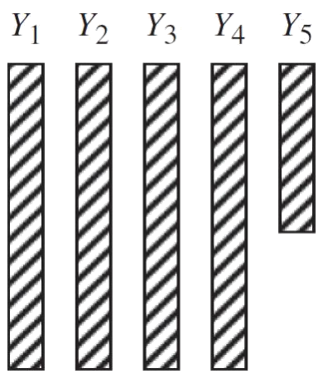
\includegraphics[width=\linewidth]{applications/figures/univariate-nonresponse.png}
        \caption{Univariate}
    \end{subfigure}
    \quad
    \begin{subfigure}{.25\textwidth}
        \centering
        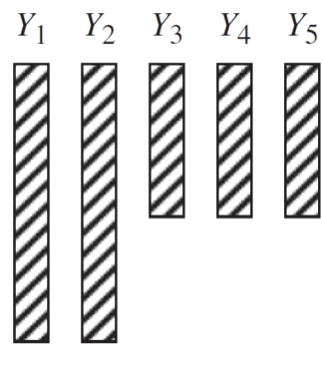
\includegraphics[width=\linewidth]{applications/figures/multivariate-nonresponse.png}
        \caption{Multivariate}
    \end{subfigure}
    \quad
    \begin{subfigure}{.25\textwidth}
        \centering
        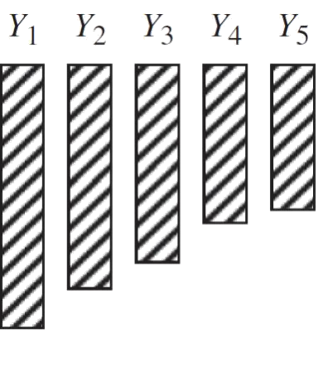
\includegraphics[width=\linewidth]{applications/figures/monotone-nonresponse.png}
        \caption{Monotone}
    \end{subfigure}
    \quad
    \begin{subfigure}{.25\textwidth}
        \centering
        
\includegraphics[width=\linewidth]{applications/figures/general-nonresponse.png}
        \caption{General}
    \end{subfigure}
    \quad
    \begin{subfigure}{.25\textwidth}
        \centering
        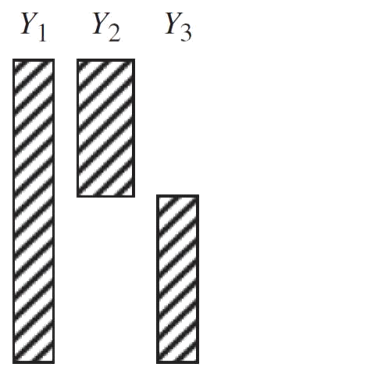
\includegraphics[width=\linewidth]{applications/figures/file-matching.png}
        \caption{File matching}
    \end{subfigure}
    \quad
    \begin{subfigure}{.25\textwidth}
        \centering
        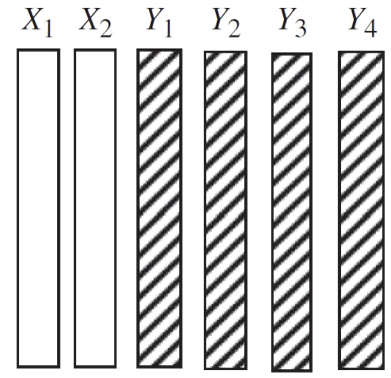
\includegraphics[width=\linewidth]{applications/figures/factor-analysis.png}
        \caption{Factor analysis}
    \end{subfigure}
    \caption{Examples of missingness patterns}
    \label{figure:examples-of-missingness-patterns}
\end{figure}

Notations for missing data are as follows
\begin{itemize}
    \item $Y=(y_{ij})$ denote the $(n\times p)$ rectangular data matrix, where only a portion of $Y$ are observed and $y_{ij}=\star$ indicates this entry is missing;
    \item $M=(m_{ij})$ denote the \textit{missingness indicator matrix} for $y_{ij}$, taking $m_{ij}=0$ for $y_{ij}$ is observed, and $m_{ij}=1$ for $y_{ij}$ is missing.
    \item In order to simplify, let $y_{i}=\left(y_{i1},y_{i2},\ldots,y_{ip}\right),\quad m_{i}=\left(m_{i1},m_{i2},\ldots,m_{ip}\right)$ and $y_{(0)i}$ be the components of $y_i$ that are observed for unit $i$, $y_{(1)i}$ be the components of $y_i$ that are missing for unit $i$.
\end{itemize}

\subsection{Missingness Mechanisms}

The missingness mechanism is characterized by the conditional distribution of $m_{i}$ given $y_{i}$, say
\begin{equation}
    f_{M\mid Y}\left(m_{i}\mid y_{i},\phi\right),
\end{equation}
where $\phi$ denotes unknown parameters.

\begin{definition}[Missing Completely at Random, MCAR]
    If missingness does not depend on the value of the data, missing or observed, i.e., if for all $y_{i}$ and any distinct values $y^{*}$ in the sample space of $Y$,
    \begin{equation}
        f_{M\mid Y}\left(m_{i} \mid y_{i},\phi\right)=f_{M\mid Y}\left(m_{i} \mid y^{*},\phi\right),
    \end{equation}
    then the data are called missing completely at random, MCAR.
\end{definition}

\begin{definition}[Missing at Random, MAR]
    If missingness depends on $y_{i}$ only through the observed components $y_{(0)}$, i.e., if for all $y_{i}$ and any distinct values $y_{(1)}^{*}$ in the sample space of $y_{(1)}$,
    \begin{equation}
        f_{M \mid Y}\left(m_{i}\mid y_{(0)i},y_{(1)i},\phi\right)=f_{M\mid Y}\left(m_{i}\mid y_{(0)i},y_{(1)}^{*},\phi\right),
    \end{equation}
    then the data are called missing at random, MAR.
\end{definition}

\begin{definition}[Missing Not at Random, MNAR]
    If missingness depends on $y_{i}$ the missing components $y_{(1)}$, i.e., if some $y_{i}$ and some values $y_{(1)}^{*}$ in the sample space of $y_{(1)}$,
    \begin{equation}
        f_{M \mid Y}\left(m_{i}\mid y_{(0)i},y_{(1)i},\phi\right)\neq f_{M\mid Y}\left(m_{i}\mid y_{(0)i},y_{(1)}^{*},\phi\right),
    \end{equation}
    then the data are called missing not at random, MNAR.
\end{definition}

\subsection{Commonly Used Methods for Missing Data}

\begin{enumerate}
    \item Complete-case Analysis: discard incompletely recorde units, only use the units with the complete data.
    \item Weighting Procedures: randomization inferences from sample survey data without nonresponse commonly weight sampled units by their design weights.
    \item Imputation Methods: impute the missing values, and the resultant completed data are analyzed by standard methods.
    \item \textbf{Model-based Methods}: A broad class of procedures is generated by defining a model for the complete data and basing inferences on the likelihood or posterior distribution under that model, with parameters estimated by procedures such as maximum likelihood.
    \item Hybrid Approaches: approaches based on estimating equations have been
          proposed that combine the aspects of modeling and weighting.
\end{enumerate}

\section{Likelihood-Based Inference with Missing Data}

We can model the density of the joint distribution of $Y$ and $M$ using the "selection model" factorization
\begin{equation*}
    p(Y=y,M=m\mid\theta,\psi)=f_{Y}(y\mid\theta)f_{M\mid Y}(m\mid y,\psi),
\end{equation*}
where $\theta$ is the parameter vector governing the data model, and $\psi$ is the parameter vector governing the model for the missingness mechanism.

The full likelihood based on the observed values $\left(y_{(0)}, m\right)$ and the assumed joint distribution model above is defined to be
\begin{equation}
    L_{\text {full }}\left(\theta, \psi \mid y_{(0)}, m\right)=\int f_{Y}\left(y_{(0)}, y_{(1)} \mid \theta\right) f_{M \mid Y}\left(m \mid y_{(0)}, y_{(1)}, \psi\right) \mathrm{d} y_{(1)}
\end{equation}

The likelihood of $\theta$ ignoring the missingness mechanism is defined to be
\begin{equation}
    L_{\mathrm{ign}}\left(\theta \mid y_{(0)}\right)=\int f_{Y}\left(y_{(0)}, y_{(1)} \mid \theta\right) \mathrm{d} y_{(1)}
\end{equation}

\subsection{Ignorable Missingness Mechanism}

\begin{definition}[Ignorable missingness mechanism]
    The missingness mechanism is called ignorable if for any given $\tilde{m}$ and  $\tilde{y}_{(0)}$ the inferences for $\theta$ based on the ignorable likelihood equation evaluated at $m=\tilde{m}$ and $\tilde{y}_{0}$ are the same as the full likelihood equation.
\end{definition}

\begin{remark}[Another definition of ignorable missingness mechanism]
    \begin{equation}
        \frac{L_{\text {full }}\left(\theta, \psi \mid \tilde{y}_{(0)}, \tilde{m}\right)}{L_{\text {full }}\left(\theta^{*}, \psi \mid \tilde{y}_{(0)}, \tilde{m}\right)}=\frac{L_{\text {ign }}\left(\theta \mid \tilde{y}_{(0)}\right)}{L_{\text {ign }}\left(\theta^{*} \mid \tilde{y}_{(0)}\right)} \quad \forall \theta, \theta^{*}, \psi .
    \end{equation}
\end{remark}

\begin{theorem}
    The missingness mechanism is ignorable for direct likelihood inference on $\left(\tilde{m},\tilde{y}_{(0)}\right)$ if
    \begin{enumerate}
        \item Parameter distinctness: The parameters $\theta$ and $\psi$ are distinct, that is, $\Omega_{\theta, \psi}=\Omega_{\theta} \times \Omega_{\psi}$.
        \item Factorization of the full likelihood: The full likelihood, with $\left(y_{0}, m\right)=\left(\tilde{y}_{0}, \tilde{m}\right)$ factors as
              \begin{equation}
                  L_{\text{full}}\left(\theta,\psi\mid\tilde{y}_{(0)},\tilde{m}\right)=L_{\text{ign}}\left(\theta\mid\tilde{y}_{(0)}\right)\times L_{\text{rest}}\left(\psi\mid\tilde{y}_{(0)},\tilde{m}\right)\quad\forall\theta,\psi\in\Omega_{\theta,\psi}
                  \label{equation:factorization-of-the-full-likelihood}
              \end{equation}
    \end{enumerate}
\end{theorem}

\begin{corollary}
    If the missing data are MAR at $\left(\tilde{m}, \tilde{y}_{(0)}\right)$, and $\theta$ and $\psi$ are distinct, the missingness mechanism is ignorable for likelihood inference.
\end{corollary}

\begin{proof}
    Since,
    \begin{equation}
        f_{M \mid Y}\left(\tilde{m} \mid \tilde{y}_{(0)}, y_{(1)}, \psi\right)=f_{M \mid Y}\left(\tilde{m} \mid \tilde{y}_{(0)}, y_{(1)}^{*}, \psi\right) \quad \forall y_{(1)}, y_{(1)}^{*}, \psi
    \end{equation}
    therefore,
    \begin{equation}
        \begin{aligned}
              & f\left(\tilde{y}_{(0)}, \tilde{m} \mid \theta, \psi\right)=f_{M \mid Y}\left(\tilde{m} \mid \tilde{y}_{(0)}, \psi\right) \times \int f_{Y}\left(\tilde{y}_{(0)}, y_{(1)} \mid \theta\right) \mathrm{d} y_{(1)} \\
            = & f_{M \mid Y}\left(\tilde{m} \mid \tilde{y}_{(0)}, \psi\right) \times f_{Y}\left(\tilde{y}_{(0)} \mid \theta\right)
        \end{aligned}
    \end{equation}
    yields the factored likelihood equation \ref{equation:factorization-of-the-full-likelihood}.
\end{proof}

\subsubsection{Ignorable Missingness Mechanism v.s. Nonignorable Missingness Mechanism}

\begin{example}[Exponential Sample]
    The joint density of $n$ independent and identically distributed scalar units from the exponential distribution with mean $\theta>0$ is
    \begin{equation}
        f_{Y}(y\mid\theta)=\theta^{-n}\exp\left\{-\sum_{i=1}^{n}\frac{y_{i}}{\theta}\right\}.
    \end{equation}

    The loglikelihood fuction is
    \begin{equation}
        \ell_{Y}(\theta\mid y)=\ln\left\{\theta^{-n}\exp\left(-\sum_{i=1}^{n}\frac{y_{i}}{\theta}\right)\right\}=-n\ln\theta-\sum_{i=1}^{n}\frac{y_{i}}{\theta}.
    \end{equation}

    Differentiating with respect to $\theta$ gives the likelihood equation
    \begin{equation}
        -\frac{n}{\theta}+\sum_{i=1}^{n} \frac{y_{i}}{\theta^{2}}=0.
    \end{equation}

    Thus, we obtain the ML estimates
    \begin{equation}
        \hat{\theta}=\bar{y}=\frac{1}{n}\sum_{i=1}^{n}y_i.
    \end{equation}
\end{example}

\begin{example}[Incomplete Exponential Sample]
    Suppose we have an incomplete univariate exponential sample with $y_{(0)}=\left(y_{1},\ldots,y_{r}\right)^{\mathrm{T}}$ observed and $y_{(1)}=\left(y_{r+1},\ldots,y_{n}\right)^{\mathrm{T}}$ missing. Thus, $m=\left(m_{1},\ldots,m_{n}\right)^{\mathrm{T}}$, where $m_{i}=0,i=1,\ldots,r$ and $m_{i}=1,i=r+1,\ldots,n$.

    The likelihood ignoring the missingness mechanism is
    \begin{equation}
        L_{\mathrm{ign}}\left(\theta\mid y_{(0)}\right)=\theta^{-r}\exp\left(-\sum_{i=1}^{r}\frac{y_{i}}{\theta}\right).
    \end{equation}

    If each unit is observed with probability $\psi$ that does not depend on $Y$, that is,
    \begin{equation}
        f_{M\mid Y}(m\mid y,\psi)=\frac{n!}{r!(n-r)!}\psi^{r}(1-\psi)^{n-r}
    \end{equation}
    then,
    \begin{equation}
        f\left(y_{(0)},m\mid\theta,\psi\right)=\frac{n!}{r!(n-r)!}\psi^{r}(1-\psi)^{n-r}\theta^{-r}\exp\left(-\sum_{i=1}^{r}\frac{y_{i}}{\theta}\right)
    \end{equation}
    Because the missing data are MAR, if $\psi$ and $\theta$ are distinct, then likelihood-based
    inferences about $\theta$ can be based on the ignorable likelihood, the ML estimate of $\theta$ is
    \begin{equation}
        \hat{\theta}=\frac{1}{r}\sum_{i=1}^{r}y_{i}.
    \end{equation}

    If each unit is observed only if values less than $c$, that is
    \begin{equation}
        f_{M\mid Y}(m\mid y,\psi)=\prod_{i=1}^{n}f\left(m_{i}\mid y_{i},\psi\right),
    \end{equation}
    where
    \begin{equation}
        f\left(m_{i} \mid y_{i}, \psi\right)=\left\{\begin{array}{ll}
            1, & y_{i}\geq c        \\
            0, & \text{ otherwise }
        \end{array}\right.
    \end{equation}
    Hence,
    \begin{equation}
        \begin{aligned}
            L_{\text {full }}\left(\theta \mid y_{(0)}, m\right) & =\prod_{i=1}^{r} f_{Y}\left(y_{i} \mid \theta\right) \operatorname{Pr}\left(y_{i}<c \mid y_{i}, \theta\right) \times \prod_{i=r+1}^{n} \operatorname{Pr}\left(y_{i} \geq c \mid \theta\right) \\
                                                                 & =\theta^{-r} \exp \left(-\sum_{1}^{r} \frac{y_{i}}{\theta}\right) \times \exp \left(-\frac{(n-r) c}{\theta}\right)
        \end{aligned}
    \end{equation}
    Maximizing above equation with respect to $\theta$ gives the ML estimate
    \begin{equation}
        \hat{\theta}=\frac{1}{r}\left[\sum_{i=1}^{r}y_{i}+(n-r)c\right].
    \end{equation}

    The inflation of the sample mean in this expression reflects the censoring of the missing values.
\end{example}

\subsection{Expectation-Maximization Algorithm}

Let $\theta^{(i)}$ be the current estimate of the parameter $\theta .$ The E step of EM finds the expected complete-data loglikelihood if $\theta$ were $\theta^{(t)}$:
\begin{equation}
    Q\left(\theta \mid \theta^{(t)}\right)=\int\ell\left(\theta \mid Y_{(0)}, Y_{(1)}\right) f\left(Y_{(1)} \mid Y_{(0)}, \theta^{(t)}\right) \mathrm{d} Y_{(1)}.
\end{equation}

The M step of EM determines $\theta^{(t+1)}$ by maximizing this expected completedata loglikelihood:
\begin{equation}
    Q\left(\theta^{(t+1)} \mid \theta^{(t)}\right) \geq Q\left(\theta \mid \theta^{(t)}\right), \quad \forall\theta.
\end{equation}

Hence, EM algorithm for likelihood-based inference with missing data is
\begin{enumerate}
    \item replace missing values by estimated
          values
    \item estimate parameters
    \item re-estimate the missing values assuming the new parameter estimates are correct
    \item re-estimate parameters, and so forth, iterating until apparent convergence
\end{enumerate}

\subsubsection{Convergence Properties of EM Algorithm with Missing Data}

\begin{theorem}
    Every GEM algorithm increases $\ell\left(\theta \mid Y_{(0)}\right)$ at each iteration, that is,
    \begin{equation}
        \ell\left(\theta^{(t+1)} \mid Y_{(0)}\right) \geq \ell\left(\theta^{(t)} \mid Y_{(0)}\right)
    \end{equation}
    , with equality if and only if
    \begin{equation}
        Q\left(\theta^{(t+1)} \mid \theta^{(t)}\right)=Q\left(\theta^{(t)} \mid \theta^{(t)}\right)
    \end{equation}
\end{theorem}

\begin{proof}
    The distribution of the complete data Y can be factored as follows:
    \begin{equation}
        f(Y \mid \theta)=f\left(Y_{(0)}, Y_{(1)} \mid \theta\right)=f\left(Y_{(0)} \mid \theta\right) f\left(Y_{(1)} \mid Y_{(0)}, \theta\right)
    \end{equation}

    The corresponding decomposition of the loglikelihood is
    \begin{equation}
        \ell(\theta \mid Y)=\ell\left(\theta \mid Y_{(0)}, Y_{(1)}\right)=\ell\left(\theta \mid Y_{(0)}\right)+\ln f\left(Y_{(1)} \mid Y_{(0)}, \theta\right)
    \end{equation}

    Let,
    \begin{equation}
        \ell\left(\theta \mid Y_{(0)}\right)=\ell(\theta \mid Y)-\ln f\left(Y_{(1)} \mid Y_{(0)}, \theta\right)
    \end{equation}

    The expectation of both sides of above equation over the distribution of the missing data $Y_{(1)}$, given the observed data $Y_{(0)}$ and a current estimate of $\theta$, say $\theta_{(t)}$, is
    \begin{equation}
        \ell\left(\theta \mid Y_{(0)}\right)=Q\left(\theta \mid \theta^{(t)}\right)-H\left(\theta \mid \theta^{(t)}\right)
    \end{equation}
    , where
    \begin{equation}
        \begin{aligned}
            Q\left(\theta \mid \theta^{(t)}\right)= & \int\ell\left(\theta \mid Y_{(0)}, Y_{(1)}\right) f\left(Y_{(1)} \mid Y_{(0)}, \theta^{(t)}\right) \mathrm{d} Y_{(1)} \\
            H\left(\theta\mid\theta^{(t)}\right)=   & \int\ln f\left(Y_{(1)}\mid Y_{(0)},\theta\right)f\left(Y_{(1)} \mid Y_{(0)}, \theta^{(t)}\right) \mathrm{d} Y_{(1)}
        \end{aligned}
    \end{equation}

    Since,
    \begin{equation}
        \begin{aligned}
                 & H\left(\theta^{(t)},\theta^{(t)}\right)-H\left(\theta,\theta^{(t)}\right)                                                                                                           \\
            =    & \int\ln f\left(Y_{(1)}\mid Y_{(0)},\theta^{(t)}\right)f\left(Y_{(1)}\mid Y_{(0)},\theta^{(t)}\right)\mathrm{d}Y_{(1)}                                                               \\
                 & -\int\ln f\left(Y_{(1)}\mid Y_{(0)},\theta\right))f\left(Y_{(1)}\mid Y_{(0)},\theta^{(t)}\right)\mathrm{d}Y_{(1)}                                                                   \\
            =    & \int\ln\left[\frac{f\left(Y_{(1)}\mid Y_{(0)},\theta^{(t)}\right)}{f\left(Y_{(1)}\mid Y_{(0)},\theta\right)}\right]f\left(Y_{(1)}\mid Y_{(0)},\theta^{(t)}\right)\mathrm{d}Y_{(1)}  \\
            =    & \int-\ln\left[\frac{f\left(Y_{(1)}\mid Y_{(0)},\theta\right)}{f\left(Y_{(1)}\mid Y_{(0)},\theta^{(t)}\right)}\right]f\left(Y_{(1)}\mid Y_{(0)},\theta^{(t)}\right)\mathrm{d}Y_{(1)} \\
            \geq & -\ln\int\frac{f\left(Y_{(1)}\mid Y_{(0)},\theta\right)}{f\left(Y_{(1)}\mid Y_{(0)},\theta^{(t)}\right)}f\left(Y_{(1)}\mid Y_{(0)},\theta^{(t)}\right)\mathrm{d}Y_{(1)}=0
        \end{aligned}
    \end{equation}

    Therefore,
    \begin{equation}
        H\left(\theta \mid \theta^{(t)}\right) \leq H\left(\theta^{(t)} \mid \theta^{(t)}\right)
    \end{equation}

    Hence, the difference in values of $\ell\left(\theta \mid Y_{(0)}\right)$ at successive iterates is given by
    \begin{equation}
        \begin{aligned}
            \ell\left(\theta^{(t+1)} \mid Y_{(0)}\right)-\ell\left(\theta^{(t)} \mid Y_{(0)}\right)= & \left[Q\left(\theta^{(t+1)} \mid \theta^{(t)}\right)-Q\left(\theta^{(t)} \mid \theta^{(t)}\right)\right]  \\
                                                                                                     & -\left[H\left(\theta^{(t+1)} \mid \theta^{(t)}\right)-H\left(\theta^{(t)} \mid \theta^{(t)}\right)\right] \\
            \geq                                                                                     & 0
        \end{aligned}
    \end{equation}
\end{proof}

\begin{theorem}
    Suppose a sequence of EM iterates is such that
    \begin{enumerate}
        \item $D^{10} Q\left(\theta^{(t+1)} \mid \theta^{(t)}\right)=0$, where "D" here denotes derivative, and $D^{10}$ means the derivative with respect to the first argument, that is, define
              \begin{equation}
                  D^{10} Q\left(\theta^{(t+1)}\mid\theta^{(t)}\right)=\left.\frac{\partial}{\partial \theta} Q\left(\theta \mid \theta^{(t)}\right)\right|_{\theta=\theta^{(t+1)}}=0.
              \end{equation}
        \item $\theta^{(t)}$ converges to $\theta^{*}$.
        \item $f\left(Y_{(1)} \mid Y_{(0)}, \theta\right)$ is smooth in $\theta$, where smooth is defined in the proof.
    \end{enumerate}
    Then
    \begin{equation}
        \left.D \ell\left(\theta^{*} \mid Y_{(0)}\right) \equiv \frac{\partial}{\partial \theta} \ell\left(\theta \mid Y_{(0)}\right)\right|_{\theta=\theta^{*}}=0,
    \end{equation}
    so that if the $\theta^{(t)}$ converge, they converge to a stationary point.
\end{theorem}

\begin{proof}
    \begin{equation}
        \begin{aligned}
            D \ell\left(\theta^{(t+1)} \mid Y_{(0)}\right) & =D^{10} Q\left(\theta^{(t+1)} \mid \theta^{(t)}\right)-D^{10} H\left(\theta^{(t+1)} \mid \theta^{(t)}\right)                                                                                       \\
                                                           & =-D^{10} H\left(\theta^{(t+1)} \mid \theta^{(t)}\right)                                                                                                                                            \\
                                                           & =-\left.\frac{\partial}{\partial \theta} \int\left[\ln f\left(Y_{(1)} \mid Y_{(0)}, \theta\right)\right] f\left(Y_{(1)} \mid Y_{(0)}, \theta^{(t)}\right) d Y_{(1)}\right|_{\theta=\theta^{(t+1)}}
        \end{aligned}
    \end{equation}
    which assuming sufficient smoothness to interchange the order of differentiation and integration,
    \begin{equation}
        \begin{aligned}
            = & -\int\left.\frac{\partial}{\partial \theta} f\left(Y_{(1)} \mid Y_{(0)}, \theta\right) d Y_{(1)}\right|_{\theta=\theta^{(t+1)}}    \\
            = & -\left.\int \frac{\partial}{\partial \theta} f\left(Y_{(1)} \mid Y_{(0)}, \theta\right) d Y_{(1)}\right|_{\theta=\theta^{(t+1)}}=0
        \end{aligned}
    \end{equation}
\end{proof}

\subsubsection{Examples of EM Algorithm with Missing Data}

\begin{example}[Multivariate Normal Sample]
    Let $y=\left(y_{i j}\right)$, where $i=1, \ldots, n$, $j=1, \ldots, p$, be a matrix representing an independent and identically distributed sample of $n$ units from the multivariate normal distribution with mean vector $\mu=\left(\mu_{1}, \ldots, \mu_{p}\right)$ and covariance matrix $\Sigma=(\sigma_{j k})$, $j=1, \ldots, p$; $k=1,\ldots, p$. Thus, $y_{i j}$ represents the value of the jth variable for the ith unit in the sample. The density of $y$ is
    \begin{equation}
        f_{Y}(y\mid\mu,\Sigma)=(2 \pi)^{-n p / 2}|\Sigma|^{-n / 2} \exp \left\{-\frac{1}{2} \sum_{i=1}^{n}\left(y_{i}-\mu\right) \Sigma^{-1}\left(y_{i}-\mu\right)^{\mathrm{T}}\right\}.
    \end{equation}

    The loglikelihood of $\theta=(\mu, \Sigma)$ is then
    \begin{equation}
        \ell_{Y}(\mu, \Sigma \mid y)=-\frac{n}{2}\ln |\Sigma|-\frac{1}{2} \sum_{i=1}^{n}\left(y_{i}-\mu\right) \Sigma^{-1}\left(y_{i}-\mu\right)^{\mathrm{T}}
    \end{equation}

    Maximizing above equation with respect to $\theta$ and $\Sigma$ gives the ML estimate
    \begin{equation}
        \hat{\mu}=\bar{y},\quad \hat{\Sigma}=\frac{n-1}{n}S,
    \end{equation}
    where $\bar{y}=\left(\bar{y}_{1}, \ldots, \bar{y}_{p}\right)$ is the row vector of sample means, and $S=\left(s_{j k}\right)$ is the $(p\times p)$ sample covariance matrix with $(j, k)$ th element $s_{j k}=\frac{1}{n-1}\sum_{i=1}^{n}\left(y_{i j}-\bar{y}_{i}\right)\left(y_{i k}-\bar{y}_{k}\right)$
\end{example}

\begin{example}[Incomplete Multivariate Normal Sample]
    Suppose $Y=\left(Y_{(0)}, Y_{(1)}\right)$, where $Y$ represents a random sample of size $n$ on $\left(Y_{1}, \ldots, Y_{p}\right), Y_{(0)}$ the set of observed values, and $Y_{(1)}$ the missing data. Also, let $y_{(0), i}$ represent the set of variables with values observed for unit $i, \quad i=1, \ldots, n$.

    The loglikelihood based on the observed data is then
    \begin{equation}
        \ell\left(\mu, \Sigma \mid Y_{(0)}\right)=-\frac{1}{2} \sum_{i=1}^{n} \ln \left|\Sigma_{(0), i}\right|-\frac{1}{2} \sum_{i=1}^{n}\left(y_{(0), i}-\mu_{(0), i}\right)^{\mathrm{T}} \Sigma_{(0), i}^{-1}\left(y_{(0), i}-\mu_{(0), i}\right)
    \end{equation}
    , where $\mu_{(0), i}$ and $\Sigma_{(0), i}$ are the mean and covariance matrix of the observed components of $Y$ for unit $i$.

    The exponential family form of multivariate normal distribution with $\left(\mu,\Sigma\right)$ is
    \begin{equation}
        f_{Y}(y\mid\mu,\Sigma)=(2\pi)^{-np/2}|\Lambda|^{n/2}\exp\left[\eta^{T}\sum_{i=1}^{n}y_{i}-\frac{1}{2}\sum_{i=1}^{n}\operatorname{tr}\left(\Lambda y_{i}y_{i}^{T}\right)-\frac{n}{2}\eta^{T}\Lambda\eta\right]
    \end{equation}
    , where $\Lambda=\Sigma^{-1}$ and $\eta=\Sigma^{-1}\mu$. And
    \begin{equation}
        \ln f_{Y}(y\mid\mu,\Sigma)=-\frac{np}{2}\ln(2\pi)+\frac{n}{2}\ln|\Lambda|-\frac{n}{2}\eta^{T}\Lambda\eta+\eta^{T}\sum_{i=1}^{n}y_{i}-\frac{1}{2}\sum_{i=1}^{n}\operatorname{tr}\left(\Lambda y_{i}y_{i}^{T}\right)
    \end{equation}

    Hence,
    \begin{equation}
        \begin{aligned}
              & Q\left(\theta\mid\theta^{(t)}\right)=E_{Y_{(0)},\theta^{(t)}}\left[\ell\left(\theta\mid Y_{(0)},Y_{(1)}\right)\right]                  \\
            = & -\frac{np}{2}\ln(2\pi)+\frac{n}{2}\ln|\Lambda|-\frac{n}{2}\eta^{T}\Lambda\eta                                                          \\
              & +\eta^{T}E\left(\sum_{i=1}^{n}y_{i}\right)-\frac{1}{2}\sum_{i=1}^{n}\operatorname{tr}\left(\Lambda E\left(y_{i}y_{i}^{T}\right)\right)
        \end{aligned}
    \end{equation}

    Therefore, the EM algorithm for incomplete multivariate normal sample is,
    \begin{itemize}
        \item E-step:
              \begin{equation}
                  \begin{aligned}
                      E\left(\sum_{i=1}^{n} y_{i j} \mid Y_{(0)}, \theta^{(t)}\right)=         & \sum_{i=1}^{n} y_{i j}^{(t+1)}, \quad j=1, \ldots, p                                                  \\
                      E\left(\sum_{i=1}^{n} y_{i j} y_{i k} \mid Y_{(0)}, \theta^{(t)}\right)= & \sum_{i=1}^{n}\left(y_{i j}^{(t+1)} y_{i k}^{(t+1)}+c_{j k i}^{(t+1)}\right), \quad j, k=1, \ldots, p
                  \end{aligned}
              \end{equation}
              where
              \begin{equation}
                  \begin{aligned}
                      y_{i j}^{(t+1)}=   & \left\{\begin{array}{ll}
                                                      y_{i j},                                             & \text { if } y_{i j} \text { is observed} \\
                                                      E\left(y_{i j} \mid y_{(0), i}, \theta^{(t)}\right), & \text { if } y_{i j} \text { is missing}
                                                  \end{array}\right.                                                                         \\
                      c_{j k i}^{(t+1)}= & \left\{\begin{array}{ll}
                                                      0,                                                                             & \text { if } y_{i j} \text { or } y_{i k} \text { is observed}  \\
                                                      \operatorname{Cov}\left(y_{i j}, y_{i k} \mid y_{(0), i}, \theta^{(t)}\right), & \text { if } y_{i j} \text { and } y_{i k} \text { are missing}
                                                  \end{array}\right.
                  \end{aligned}
              \end{equation}

        \item M-step:
              \begin{equation}
                  \begin{aligned}
                      \mu_{j}^{(t+1)}      & =n^{-1} \sum_{i=1}^{n} y_{i j}^{(t+1)}, \quad j=1, \ldots, p                                                                                                           \\
                      \sigma_{j k}^{(t+1)} & =n^{-1} E\left(\sum_{i=1}^{n} y_{i j} y_{i k} \mid Y_{(0)}, \theta^{(t)}\right)-\mu_{j}^{(t+1)} \mu_{k}^{(t+1)}                                                        \\
                                           & =n^{-1} \sum_{i=1}^{n}\left[\left(y_{i j}^{(t+1)}-\mu_{j}^{(t+1)}\right)\left(y_{i k}^{(t+1)}-\mu_{k}^{(t+1)}\right)+c_{j k i}^{(t+1)}\right], \quad j, k=1, \ldots, p
                  \end{aligned}
              \end{equation}
    \end{itemize}
\end{example}

\begin{example}[Missing Outcomes in Multiple Linear Regression]
    Suppose a scalar outcome variable $Y$ is regressed on $p$ predictor variables $X_{1},\ldots,X_{p}$, $y_{i},i=1,\ldots,m$ are missing, where
    \begin{equation}
        \begin{aligned}
            E\left(Y \mid X_{1}, \ldots, X_{p}\right)                  & =\beta_{0}+\sum_{j=1}^{p} \beta_{j} X_{j} \\
            \operatorname{Var}\left(Y \mid X_{1}, \ldots, X_{p}\right) & =\sigma^{2}
        \end{aligned}
    \end{equation}

    We assume the joint distribution of the data (including outcomes and predictors) is multivariate normal with
    \begin{equation}
        \begin{aligned}
            \mu    & =\left(\mu_{1}, \ldots, \mu_{p}, \mu_{y}\right) \\
            \Sigma & =\left(\begin{array}{ll}
                                    \Sigma_{x x} & \Sigma_{x y} \\
                                    \Sigma_{y x} & \sigma_{y y}
                                \end{array}\right)
        \end{aligned}
    \end{equation}
    , and that the missing data mechanism is ignorable.

    Standard regression theory gives
    \begin{equation}
        \begin{array}{c}
            \beta=\boldsymbol{\Sigma}_{y x} \boldsymbol{\Sigma}_{x x}^{-1} ; \quad \beta_{0}=\mu_{y}-\sum_{j=1}^{p} \beta_{j} \mu_{j} ; \\
            \sigma^{2}=\sigma_{y y}-\boldsymbol{\Sigma}_{y x} \boldsymbol{\Sigma}_{x x}^{-1} \boldsymbol{\Sigma}_{x y}
        \end{array}
    \end{equation}

    The loglikelihood based on the observed data of $\theta=\left(\beta,\sigma^{2}\right)$, where $\beta=\left(\beta_{0},\beta_{1},\ldots,\beta_{p}\right)$, given observed data $\left\{\left(x_{i},y_{i}\right),i=1,\ldots,n\right\}$ is
    \begin{equation}
        \ell(\beta, \sigma^{2} \mid X, Y_{(0)})=-\frac{n-m}{2}\ln\sigma^2-\frac{1}{2}\sum_{i=m+1}^{n}\left(y_{i}-\beta_{0}-\sum_{j=1}^{p}x_{ij}\beta_{j}\right)^2
    \end{equation}
    , where only using the observed data.

    EM algorithms can be applied to all observations and will obtain iteratively the same ML estimates as would have been obtained noniteratively using only the complete observations.

    \begin{itemize}
        % 给出 Q(\theta) 的表达式
        \item E-step:
              \begin{equation}
                  \begin{aligned}
                      E\left(y_{i} \mid X, Y_{(0)}, \theta^{(t)}\right)=     & \left\{\begin{array}{ll}
                                                                                          y_{i},                                 & \text { if } y_{i} \text { is observed } \\
                                                                                          \beta^{(t)} \tilde{x}_{i}^{\mathrm{T}} & \text { if } y_{i} \text { is missing }
                                                                                      \end{array}\right.                                                                                                          \\
                      E\left(y_{i}^{2} \mid X, Y_{(0)}, \theta^{(t)}\right)= & \left\{\begin{array}{ll}
                                                                                          y_{i}^{2},                                                                & \text { if } y_{i} \text { is observed } \\
                                                                                          \left(\beta^{(t)} \tilde{x}_{i}^{\mathrm{T}}\right)^{2}+\sigma^{(t)^{2}}, & \text { if } y_{i} \text { is missing }
                                                                                      \end{array}\right.
                  \end{aligned}
              \end{equation}
              , where $\tilde{x}_{i}=(1,x_{i})$.
        \item M-step:
              \begin{equation}
                  \begin{aligned}
                      \beta^{(t+1)}=      & \left(X^{\mathrm{T}} X\right)^{-1} X^{\mathrm{T}} Y^{(t+1)}                                    \\
                      \sigma^{(t+1)^{2}}= & n^{-1}\left[\sum_{i=m+1}^{n}\left(y_{i}-\beta^{(t)} x_{i}\right)^{2}+m \sigma^{(t)^{2}}\right] \\
                  \end{aligned}
              \end{equation}
              , where $X=(1,X_1,X_2,\ldots,X_p)$
    \end{itemize}
\end{example}

\section{Missing Not At Random Models}

Here, we based on
\begin{equation}
    L_{\text {full }}\left(\theta, \psi \mid Y_{(0)}, X, M\right) \propto f\left(Y_{(0)}, M \mid X, \theta, \psi\right)
\end{equation}
regarded as a function of the parameters $\theta, \psi$ for fixed observed data $Y_{(0)}$ and missingness pattern $M$; here $f\left(Y_{(0)}, M \mid X, \theta, \psi\right)$ is obtained by integrating $Y_{(1)}$ out of the joint density $f(Y, M \mid X, \theta, \psi)$ based on a joint model for $Y$ and $M$ given $X$.

The EM algorithm has the following form for MNAR selection models are as followed,
\begin{itemize}
    \item E-step:
          \begin{equation}
              \begin{aligned}
                  Q\left(\theta, \psi \mid \theta^{(t)}, \psi^{(t)}\right)= & \int \ell\left(\theta, \psi \mid X, Y_{(0)}, Y_{(1)}, M\right)                                         \\
                                                                            & \cdot f\left(Y_{(1)}\mid X, Y_{(0)}, M, \theta=\theta^{(t)}, \psi=\psi^{(t)}\right) \mathrm{d} Y_{(1)}
              \end{aligned}
          \end{equation}
    \item M-step:
          \begin{equation}
              Q\left(\theta^{(t+1)}, \psi^{(t+1)} \mid \theta^{(t)}, \psi^{(t)}\right) \geq Q\left(\theta, \psi \mid \theta^{(t)}, \psi^{(t)}\right) \quad \text { for all } \theta, \psi
          \end{equation}
\end{itemize}

\subsection{Normal Models for MNAR Missing Data}

\begin{enumerate}
    \item Follow up a sample of nonrespondents, and incorporate this information into the main analysis.
    \item Adopt a Bayesian approach, assigning the parameters prior distributions. Bayesian inference does not generally require that the data provide information for all the parameters, although inferences tend to be sensitive to
          the choice of prior distribution.
    \item Impose additional restrictions onmodel parameters.
    \item Conduct analysis to assess sensitivity of inferences for quantities of interest to different choices of the values of parameters poorly estimated from the data.
    \item Selectively discard data to avoid modeling the missingness mechanism.
\end{enumerate}
\chapter{Treatment-effects Analysis}

\section{Evaluations}

\subsection{Average Treatment Effect}

\begin{definition}[Average Treatment Effect]
    \begin{equation}
        \operatorname{E}\left(Y_{1}-Y_{2}\right)
    \end{equation}
\end{definition}

\subsection{Mann-Whitney Statistic}

\begin{definition}[Mann-Whitney Statistic]
    \begin{equation}
        \operatorname{Pr}\left(Y_{1}<Y_{2}\right)
    \end{equation}
\end{definition}

\subsection{Distribution-type Index}

\begin{definition}[Distribution-type Index]
    \begin{equation}
        F(x):=\operatorname{Pr}\left(Y_{1}-Y_{2}=x\right)
    \end{equation}
\end{definition}


\appendix

\backmatter
\nocite{*}
\printbibliography

\end{document}